\documentclass[USenglish]{ifimaster}  %% ... or USenglish or norsk or nynorsk
\usepackage[utf8]{inputenc}           %% ... or latin1 or applemac
\usepackage[T1]{fontenc,url}
\urlstyle{sf}
\usepackage{babel,textcomp,csquotes,duomasterforside,varioref,graphicx}
\usepackage[backend=biber,style=numeric-comp]{biblatex}
\usepackage[acronym, xindy]{glossaries}
\usepackage[version=3]{mhchem}

\usepackage{array}
\usepackage{parskip}

%% Code
\usepackage{listings}
\usepackage{color}
\usepackage[pdftex]{xcolor}
\usepackage{textcomp}
\usepackage[T1]{fontenc}
\usepackage{caption}
\usepackage[hidelinks]{hyperref}
\usepackage{float}

\definecolor{jskeywords}{HTML}{E4D00A}% JavaScript keywords
\definecolor{jsextkeywords}{HTML}{FF6700}% JavaScript extended keywords

\definecolor{identifiers}{HTML}{645452} % identfiers
\definecolor{string}{HTML}{B57281} % string literals
\definecolor{allcomment}{HTML}{808080} % comment

\definecolor{nodejs}{HTML}{629755} % Nodejs keywords
\definecolor{testing}{HTML}{4169E1} % Node.js assert, jasmine
\definecolor{express}{HTML}{FF8C69} % Express.js
\definecolor{linenumber}{HTML}{996515} % line number
\definecolor{apricot}{HTML}{98777B} % numbers
\definecolor{linenofill}{HTML}{BEBEBE} % line number fill color
\definecolor{antiquefuchsia}{HTML}{915C83} % braces
\definecolor{ballblue}{HTML}{21ABCD} % braces

\definecolor{captioncolor}{rgb}{0.39, 0.33, 0.32} % caption color
\captionsetup[lstlisting]{font={color=captioncolor, small,tt}}

\captionsetup[lstlisting]{font={color=captioncolor, small, tt}}
\DeclareCaptionFormat{listing}{\rule{\dimexpr\textwidth+17pt\relax}{0.4pt}\vskip1pt#1#2#3}
\captionsetup[lstlisting]{format=listing,singlelinecheck=false, margin=0pt, font={sf},labelsep=space,labelfont=bf}

\lstdefinelanguage{JavaScript}{
  alsoletter={.},
  keywords={arguments,await,break,case,catch,class,const,continue,debugger,default,delete,do,else,enum,eval,export,extends,false,finally,for,function,if,implements,import,in,instanceof,interface,let,new,null,package,private,protected,public,return,static,super,switch,this,throw,true,try,typeof,var,void,while,with,yield}, % JavaScript ES6 keywords
  keywordstyle=\color{jskeywords}\bfseries,
  ndkeywords={add, apply, args, Array, Array.from, Array.isArray, Array.of , Array.prototype, ArrayBuffer, bind, Boolean, call, charAt, charCodeAt, clear, codePointAt, concat, constructor, copyWithin, DataView, Date, Date.now, Date.parse, Date.prototype, Date.UTC, decodeURI, decodeURIComponent, encodeURI, encodeURIComponent, endsWith, entries, Error, Error.prototype, EvalError, every, false, fill, filter, find, findIndex, Float32Array, Float64Array, forEach, FulfillPromise, Function, Function.length, get, getDate, getDay, getFullYear, getHours, getMilliseconds, getMinutes, getMonth, getSeconds, getTime, getTimezoneOffset, getUTCDate, getUTCDay, getUTCFullYear, getUTCHours, getUTCMilliseconds, getUTCMinutes, getUTCMonth, getUTCSeconds, has,hasInstance, hasOwnProperty, ignoreCase, includes, indexOf, indexOf, Infinity, Int8Array, Int16Array, Int32Array, isConcatSpreadable, isFinite, isNaN, IsPromise, isPrototypeOf, Iterable, iterator, join, JSON, JSON.parse, JSON.stringify, keys, lastIndexOf, lastIndexOf, length, localeCompare, map, Map, match, match, Math, Math.abs , Math.acos, Math.acosh, Math.asin, Math.asinh, Math.atan, Math.atan2, Math.atanh, Math.cbrt, Math.ceil, Math.clz32, Math.cos, Math.cosh,  Math.E, Math.exp, Math.expm1, Math.floor, Math.fround, Math.hypot, Math.imul, Math.LN2, Math.LN10, Math.log, Math.log1p, Math.log2, Math.LOG2E, Math.log10, Math.LOG10E, Math.max, Math.min, Math.PI, Math.pow, Math.random, Math.round, Math.sign, Math.sin, Math.sinh, Math.sqrt, Math.SQRT1_2, Math.SQRT2, Math.tan, Math.tanh, Math.trunc, message, multiline, name, NaN, NewPromiseCapability, next, normalize, null, Number, Number.EPSILON, Number.isFinite, Number.isInteger, Number.isNaN, Number.isSafeInteger, Number.MAX_SAFE_INTEGER, Number.MAX_VALUE, Number.MIN_SAFE_INTEGER, Number.MIN_VALUE, Number.NaN, Number.NEGATIVE_INFINITY, Number.parseFloat, Number.parseInt, Number.POSITIVE_INFINITY, Number.prototype, Object, Object, Object.assign, Object.create, Object.defineProperties, Object.defineProperty, Object.freeze, Object.getOwnPropertyDescriptor, Object.getOwnPropertyNames, Object.getOwnPropertySymbols, Object.getPrototypeOf, Object.is, Object.isExtensible, Object.isFrozen, Object.isSealed, Object.keys, Object.preventExtensions, Object.prototype, Object.seal, Object.setPrototypeOf, of, parseFloat, parseInt, pop, Promise, Promise.all , Promise.race, Promise.reject, Promise.resolve, PromiseReactionJob, propertyIsEnumerable, prototype, Proxy, Proxy.revocable , push, RangeError, reduce, reduceRight, ReferenceError, Reflect, Reflect.apply, Reflect.construct , Reflect.defineProperty, Reflect.deleteProperty, Reflect.enumerate, Reflect.get, Reflect.getOwnPropertyDescriptor, Reflect.getPrototypeOf, Reflect.has, Reflect.isExtensible, Reflect.ownKeys, Reflect.preventExtensions, Reflect.set, Reflect.setPrototypeOf, Reflection, RegExp, RegExp, RegExp.prototype, repeat, replace, replace, reverse, search, search, Set, set, setDate, setFullYear, setHours, setMilliseconds, setMinutes, setMonth, setSeconds, setTime, setUTCDate, setUTCFullYear, setUTCHours, setUTCMilliseconds, setUTCMinutes, setUTCMonth, setUTCSeconds, shift, slice, slice, some, sort, species, splice, split, split, startsWith, String, String.fromCharCode, String.fromCodePoint, String.raw, substring, Symbol, Symbol.for, Symbol.hasInstance, Symbol.isConcatSpreadable, Symbol.iterator, Symbol.keyFor, Symbol.match, Symbol.prototype, Symbol.replace, Symbol.replace, Symbol.search, Symbol.species, Symbol.split, Symbol.toPrimitive, Symbol.toStringTag, Symbol.unscopables, SyntaxError, then, toDateString, toExponential, toFixed, toISOString, toJSON, toLocaleDateString, toLocaleLowerCase, toLocaleString, toLocaleString, toLocaleString, toLocaleString, toLocaleTimeString, toLocaleUpperCase, toLowerCase, toPrecision, toPrimitive, toString, toStringTag, toTimeString, toUpperCase, toUTCString, TriggerPromiseReactions, trim, true, TypeError, Uint8Array, Uint8ClampedArray, Uint16Array, Uint32Array, undefined, unscopables, unshift, URIError, valueOf, WeakMap, WeakSet
  }, % JavaScript extended keywords
  ndkeywordstyle=\color{jsextkeywords}\bfseries,
  identifierstyle=\color{identifiers},
  sensitive=true,
  stringstyle=\color{string}\ttfamily,
  morestring=[b]",
  morestring=[d]',
  morestring=[s][\color{string}\ttfamily]{`}{`},
  commentstyle=\color{red}\itshape,
  morecomment=[l][\color{allcomment}]{//},
  morecomment=[s][\color{allcomment}]{/*}{*/},
  morecomment=[s][\color{allcomment}]{/**}{*/},
  emph={app.all, app.delete, app.disable, app.disabled, app.enable, app.enabled, app.engine, app.get, app.listen, app.locals, app.METHOD, app.mountpath, app.param, app.path, app.post, app.put, app.render, app.route, app.set, app.use, express, express.Router, express.static, req.acceptLanguages, req.accepts, req.acceptsCharsets, req.acceptsEncodings, req.app, req.baseUrl, req.body, req.cookies, req.fresh, req.get, req.hostname, req.ip, req.ips, req.is, req.method, req.originalUrl, req.param, req.params, req.path, req.protocol, req.query, req.range, req.route, req.secure, req.signedCookies, req.stale, req.subdomains, req.xhr, res.app, res.append, res.attachment, res.clearCookie, res.cookies, res.download, res.end, res.format, res.get, res.headersSent, res.json, res.jsonp, res.links, res.locals, res.location, res.redirect, res.render, res.sendFile, res.sendStatus, res.set, res.status, res.type, res.vary, router.all, router.METHOD, router.param, router.route, router.use}, % express keywords
  emph={[2]agent.createConnection, agent.destroy, agent.freeSockets, agent.getName, agent.maxFreeSockets, agent.maxSockets, agent.requests, agent.sockets, certificate.exportChallenge, certificate.exportPublicKey, certificate.verifySpkac, child.channel, child.connected, child.disconnect, child.kill, child.pid, child.send, child.stderr, child.stdin, child.stdio, child.stdout, child_process.exec, child_process.execFile, child_process.execFileSync, child_process.execSync, child_process.fork, child_process.spawn, child_process.spawnSync, cipher.final, cipher.getAuthTag, cipher.setAAD, cipher.setAutoPadding, cipher.update, clearImmediate, clearImmediate, clearInterval, clearInterval, clearTimeout, clearTimeout, console, console.assert, console.dir, console.error, console.info, console.log, console.time, console.timeEnd, console.trace, console.warn, decipher.final, decipher.setAAD, decipher.setAuthTag, decipher.setAutoPadding, decipher.update, dgram.createSocket, dgram.createSocket, diffieHellman.computeSecret, diffieHellman.generateKeys, diffieHellman.getGenerator, diffieHellman.getPrime, diffieHellman.getPrivateKey, diffieHellman.getPublicKey, diffieHellman.setPrivateKey, diffieHellman.setPublicKey, diffieHellman.verifyError, dns.getServers, dns.getServers, dns.lookup, dns.lookup, dns.lookupService, dns.resolve, dns.resolve4, dns.resolve6, dns.resolveCname, dns.resolveMx, dns.resolveNaptr, dns.resolveNs, dns.resolvePtr, dns.resolveSoa, dns.resolveSrv, dns.resolveTxt, dns.reverse, dns.setServers, ecdh.computeSecret, ecdh.generateKeys, ecdh.getPrivateKey, ecdh.getPublicKey, ecdh.setPrivateKey, ecdh.setPublicKey, error.address, error.code, error.errno, error.message, error.path, error.port, error.stack, error.syscall, exports, fs.access, fs.accessSync, fs.appendFile, fs.appendFileSync, fs.chmod, fs.chmodSync, fs.chown, fs.chownSync, fs.close, fs.closeSync, fs.constants, fs.createReadStream, fs.createWriteStream, fs.exists, global, http.createServer, http.get, http.globalAgent, http.request, https.createServer, https.get, https.globalAgent, https.request, message.destroy, message.headers, message.httpVersion, message.method, message.rawHeaders, message.rawTrailers, message.setTimeout, message.socket, message.statusCode, message.statusMessage, message.trailers, message.url, module, module.children, module.exports, module.filename, module.id, module.loaded, module.parent, module.require, os.arch, os.constants, os.cpus, os.endianness, os.EOL, os.freemem, os.homedir, os.hostname, os.loadavg, os.networkInterfaces, os.platform, os.release, os.tmpdir, os.totalmem, os.type, os.uptime, os.userInfo, path.basename, path.delimiter, path.dirname, path.extname, path.format, path.isAbsolute, path.join, path.normalize, path.parse, path.posix, path.relative, path.resolve, path.sep, path.win32, process, process.abort, process.arch, process.argv, process.argv0, process.channel, process.chdir, process.config, process.connected, process.cpuUsage, process.cwd, process.disconnect, process.emitWarning, process.env, process.execArgv, process.execPath, process.exit, process.exitCode, process.getegid, process.geteuid, process.getgid, process.getgroups, process.getuid, process.hrtime, process.initgroups, process.kill, process.mainModule, process.memoryUsage, process.nextTick, process.pid, process.platform, process.release, process.send, process.setegid, process.seteuid, process.setgid, process.setgroups, process.setuid, process.stderr, process.stdin, process.stdout, process.title, process.umask, process.uptime, process.version, process.versions, querystring.escape, querystring.parse, querystring.stringify, querystring.unescape, r.clearLine, readable.pause, readable.pipe, readable.push, readable.push, readable.read, readable.read, readable.resume, readable.setEncoding, readable.unpipe, readable.unshift, readable.wrap, readable._read, readStream.bytesRead, readStream.isRaw, readStream.path, readStream.setRawMode, repl.start, request.abort, request.aborted, request.end, request.flushHeaders, request.setNoDelay, request.setSocketKeepAlive, request.setTimeout, request.write, require, require.cache, require.extensions, response.addTrailers, response.end, response.finished, response.getHeader, response.getHeaderNames, response.getHeaders, response.hasHeader, response.headersSent, response.removeHeader, response.sendDate, response.setHeader, response.setTimeout, response.statusCode, response.statusMessage, response.write, response.writeContinue, response.writeHead, rl.clearScreenDown, rl.close, rl.createInterface, rl.cursorTo, rl.emitKeypressEvents, rl.moveCursor, rl.pause, rl.prompt, rl.question, rl.resume, rl.setPrompt, rl.write, script.runInNewContext, script.runInThisContext, server.addContext, server.address, server.address, server.close, server.close, server.connections, server.getTicketKeys, server.listen, server.listen, server.setTicketKeys, server.setTimeout, server.setTimeout, server.timeout, server.timeout, setImmediate, setInterval, setTimeout, socket.addMembership, socket.address, socket.bind, socket.bind, socket.close, socket.dropMembership, socket.ref, socket.send, socket.setBroadcast, socket.setMulticastLoopback, socket.setMulticastTTL, socket.setTTL, socket.unref, stream.Readable, stringDecoder.end, stringDecoder.write, timeout.ref, timeout.unref, tls.connect, tls.createSecureContext, tls.createServer, tls.getCiphers, tlsSocket.address, tlsSocket.authorizationError, tlsSocket.authorized, tlsSocket.encrypted, tlsSocket.getCipher, tlsSocket.getEphemeralKeyInfo, tlsSocket.getPeerCertificate, tlsSocket.getProtocol, tlsSocket.getSession, tlsSocket.getTLSTicket, tlsSocket.localAddress, tlsSocket.localPort, tlsSocket.remoteAddress, tlsSocket.remoteFamily, tlsSocket.remotePort, tlsSocket.renegotiate, tlsSocket.setMaxSendFragment, transform._flush, transform._transform, util.debuglog, util.deprecate, util.format, util.inherits, util.inspect, v8.getHeapStatistics, v8.setFlagsFromString, vm.createContext, vm.isContext, vm.runInContext, vm.runInDebugContext, vm.runInNewContext, vm.runInThisContext, watcher.close, worker.disconnect, worker.exitedAfterDisconnect, worker.id, worker.isConnected, worker.isDead, worker.kill, worker.process, worker.send, worker.suicide, writable.cork, writable.end, writable.setDefaultEncoding, writable.write, writeStream.bytesWritten, writeStream.columns, writeStream.path, writeStream.rows, zlib, zlib.createGunzip, zlib.createGzip, zlib.createInflate, zlib.createInflateRaw, zlib.createUnzip, zlib.deflate, zlib.deflateRaw, zlib.deflateRawSync, zlib.deflateSync, zlib.gunzip, zlib.gunzipSync, zlib.gzip, zlib.gzipSync, zlib.inflate, zlib.inflateRaw, zlib.inflateRawSync, zlib.inflateSync, zlib.unzip, zlib.unzipSync, __dirname, __filename}, % Node.js keywords
  emph={[3] assert, assert.deepEqual, assert.deepStrictEqual, assert.doesNotThrow, assert.equal, assert.fail, assert.ifError, assert.notDeepEqual, assert.notDeepStrictEqual, assert.notEqual, assert.notStrictEqual, assert.ok, assert.strictEqual, assert.throws, describe, toBe, it, xdescribe, beforeEach, afterEach, beforeAll, afterAll, expect, it, xit, xdiscribe, pending, and.callThrough, and.returnValue, and.returnValues, and.callFake, and.throwError, and.stub, .not, .calls.any, .calls.count, .calls.argsFor, .calls.allArgs, .calls.all, .calls.mostRecent, .calls.first, .calls.reset, jasmine.createSpy, jasmine.createSpyObj, jasmine.any, jasmine.anything, jasmine.objectContaining, jasmine.arrayContaining, jasmine.stringMatching, asymmetricMatch,  jasmine.clock, .not.toBeTruthy, .toBeTruthy, .not.toBeFalsy, .toBeFalsy, .not.toBeDefined .toBeDefined, .not.toBeNull .toBeNull, .not.toEqual .toEqual, .not.toBeCloseTo .toBeCloseTo, .not.toContain, .toContain, .not.toMatch, .toMatch, .not.toBeGreaterThan, .toBeGreaterThan, .not.toBeLessThan, .toBeLessThan, .toThrow, .not.toThrow, .toBeNull, .not.toBeNull, .toBeDefined, .not.toBeDefined}, % Node.js Assert, Jasmine, ... keywords
  }

  \lstset{
   basicstyle=\normalsize\linespread{1.1}\footnotesize\ttfamily,
   language=JavaScript,
   frame=top,frame=bottom,
   breaklines=true,
   showstringspaces=false,
   tabsize=2,
   upquote = true,
   numbers=left,
   numberstyle=\tiny,
   stepnumber=1,
   numbersep=5pt,
   numberblanklines=false,
   xleftmargin=17pt,
   framexleftmargin=17pt,
   framexrightmargin=17pt,
   framexbottommargin=5pt,
   framextopmargin=5pt,
   alsoother={.},
   captionpos=t,
   literate=
            *{\{}{{\textcolor{antiquefuchsia}{\{}}}{1}% punctuators
            {\}}{{\textcolor{antiquefuchsia}{\}}}}{1}%
            {(}{{\textcolor{antiquefuchsia}{(}}}1%
            {)}{{\textcolor{antiquefuchsia}{)}}}1%
            {[}{{\textcolor{antiquefuchsia}{[}}}1%
            {]}{{\textcolor{antiquefuchsia}{]}}}1%
            {...}{{\textcolor{ballblue}{...}}}1%
            {;}{{\textcolor{antiquefuchsia}{;}}}1%
            {,}{{\textcolor{antiquefuchsia}{,}}}1%
            {>}{{\textcolor{ballblue}{>}}}1%
            {<}{{\textcolor{ballblue}{<}}}1%
            {<=}{{\textcolor{ballblue}{<=}}}1%
            {>=}{{\textcolor{ballblue}{>=}}}1%
            {==}{{\textcolor{ballblue}{==}}}1%
            {!=}{{\textcolor{ballblue}{!=}}}1%
            {===}{{\textcolor{ballblue}{===}}}1%
            {!==}{{\textcolor{ballblue}{!==}}}1%
            {+}{{\textcolor{ballblue}{+}}}1%
            {-}{{\textcolor{ballblue}{-}}}1%
            {*}{{\textcolor{ballblue}{*}}}1%
            {\%}{{\textcolor{ballblue}{\%}}}1%
            {++}{{\textcolor{ballblue}{++}}}1%
            {--}{{\textcolor{ballblue}{--}}}1%
            {<<}{{\textcolor{ballblue}{<<}}}1%
            {>>}{{\textcolor{ballblue}{>>}}}1%
            {>>>}{{\textcolor{ballblue}{>>>}}}1%
            {=}{{\textcolor{ballblue}{=}}}1%
            {&}{{\textcolor{ballblue}{&}}}1%
            {|}{{\textcolor{ballblue}{|}}}1%
            {^}{{\textcolor{ballblue}{^}}}1%
            {!}{{\textcolor{ballblue}{!}}}1%
            {~}{{\textcolor{ballblue}{~}}}1%
            {&&}{{\textcolor{ballblue}{&&}}}1%
            {||}{{\textcolor{ballblue}{||}}}1%
            {?}{{\textcolor{ballblue}{?}}}1%
            {:}{{\textcolor{ballblue}{:}}}1%
            {=}{{\textcolor{ballblue}{=}}}1%
            {+=}{{\textcolor{ballblue}{+=}}}1%
            {-=}{{\textcolor{ballblue}{-=}}}1%
            {*=}{{\textcolor{ballblue}{*=}}}1%
            {\%=}{{\textcolor{ballblue}{\%=}}}1%
            {<<=}{{\textcolor{ballblue}{<<=}}}1%
            {>>=}{{\textcolor{ballblue}{>>=}}}1%
            {>>>=}{{\textcolor{ballblue}{>>>=}}}1%
            {&=}{{\textcolor{ballblue}{&=}}}1%
            {|=}{{\textcolor{ballblue}{|=}}}1%
            {^=}{{\textcolor{ballblue}{^=}}}1%
            {=>}{{\textcolor{ballblue}{=>}}}1%
            {\\b}{{\textcolor{ballblue}{\\b}}}1% escape sequences
            {\\t}{{\textcolor{apricot}{\\t}}}{1}%
            {\\n}{{\textcolor{apricot}{\\n}}}{1}%
            {\\v}{{\textcolor{apricot}{\\v}}}{1}%
            {\\f}{{\textcolor{apricot}{\\f}}}{1}%
            {\\r}{{\textcolor{apricot}{\\r}}}{1}%
            {\\"}{{\textcolor{apricot}{\\"}}}{1}%
            {\\'}{{\textcolor{apricot}{\\'}}}{1}%
            {\\}{{\textcolor{apricot}{\\}}}{1}%
            {0}{{\textcolor{apricot}{0}}}{1}% numbers
            {1}{{\textcolor{apricot}{1}}}{1}%
            {2}{{\textcolor{apricot}{2}}}{1}%
            {3}{{\textcolor{apricot}{3}}}{1}%
            {4}{{\textcolor{apricot}{4}}}{1}%
            {5}{{\textcolor{apricot}{5}}}{1}%
            {6}{{\textcolor{apricot}{6}}}{1}%
            {7}{{\textcolor{apricot}{7}}}{1}%
            {8}{{\textcolor{apricot}{8}}}{1}%
            {9}{{\textcolor{apricot}{9}}}{1}%
            {.0}{{\textcolor{apricot}{.0}}}{2}%
            {.1}{{\textcolor{apricot}{.1}}}{2}%
            {.2}{{\textcolor{apricot}{.2}}}{2}%
            {.3}{{\textcolor{apricot}{.3}}}{2}%
            {.4}{{\textcolor{apricot}{.4}}}{2}%
            {.5}{{\textcolor{apricot}{.5}}}{2}%
            {.6}{{\textcolor{apricot}{.6}}}{2}%
            {.7}{{\textcolor{apricot}{.7}}}{2}%
            {.8}{{\textcolor{apricot}{.8}}}{2}%
            {.9}{{\textcolor{apricot}{.9}}}{2},%
   emphstyle={\color{express}}, % express
   emphstyle={[2]\color{nodejs}}, % node.js
   emphstyle={[3]\color{testing}}, % jasmine ...
   numberstyle=\normalfont\tiny\textcolor{linenumber} % line number
}

%% Set text area of A4 paper
%%\usepackage[a4paper, total={6in, 8in}]{geometry}
\makeglossaries{}

\title{\acrlong{nb-iot}}        %% ... or whatever
\subtitle{INTRODUCTION AND INVESTIGATION}         %% ... if any
\author{Henning Håkonsen}             %% ... or whoever

\bibliography{mybib}                  %% Load bib

\loadglsentries[main]{glossary}       %% Load glossary from file
\begin{document}

\duoforside[dept={Department of Informatics},   %% ... or your department
  program={Network and system administration},  %% ... or your programme
  long]                                        %% ... or long

\frontmatter{}
\chapter*{Abstract}                   %% ... or Sammendrag or Samandrag

\tableofcontents{}
\listoffigures{}
\listoftables{}

\chapter*{Preface}                    %% ... or Forord

\mainmatter{}
\part{Introduction}                   %% ... or Innledning or Innleiing

\chapter{Background}                  %% ... or Bakgrunn
Today there are approximately 30 billion smart devices in the world. The growth forwards will be exponential and analysis predict that there will be 50 billion smart devices by 2020 \cite{online:IoT2020}. There is a demand for a new technology which enables communication with sensors and other low powered devices. We will introduce you to a set of technologies suited for this communication, with an emphasis on \acrfull{nb-iot}. We are at a point where \acrshort{iot} is becoming a part of our society which enhances our life experience.

\section{Goal of the thesis}
The goal of this thesis is to show you how \acrshort{iot} will become a part our lives. We will discuss \acrshort{iot} applications, upcoming \acrshort{iot} technologies and how they differ. The main topic of this thesis is \acrshort{nb-iot} and how it performs in regard to its specification. There are several claims to this technology, battery lifetime over 10 years, indoor and underground coverage and low cost. Through a cooperation with Q-Free and Telenor we will be able to get hands on tests of \acrshort{nb-iot}. The interesting part of this thesis is that we are the first to really test \acrshort{nb-iot} and this gives us an opportunity to verify the specifications without to much interference. There are several papers on how \acrshort{nb-iot} has great power saving features, referring to the \acrshort{3gpp} specification, but there are not many discussing how they can be achieved in practice. Several factors will influence the power usage, such as environmental changes, downtime in the network, network configurability and software complexity. We will show you how these factors impact the power consumption and try to give an overview of the best practice usage.

\section{Motivation}
Easily accessed information, connected to all parts of society is a huge motivator for \acrfull{iot}. In the future all things will be connected to the Internet, enhancing our lives. The meaning of \acrshort{iot} is a group of physical devices, for example vehicles, monitoring systems, watches and so forth, forming a network. The complexity and possibilities with this kind of network are incredible. However, the path towards this goal has not been easy. There has been attempts of similar networks, but they usually are to fixed, expensive and the competition has been more of an obstacle than an advantage. With to many poor solutions the growth has been rather low compared to what we now see a start to. With several emerging technologies suited for low powered devices we expect a huge growth. Based on numbers from an article anticipating the growth of the population by The United Nations \cite{online:pop2300}, Cisco has made an illustration of the expected growth of devices towards 2020 \vref{pic:IoT2020}.

\begin{figure}[ht]
  \centering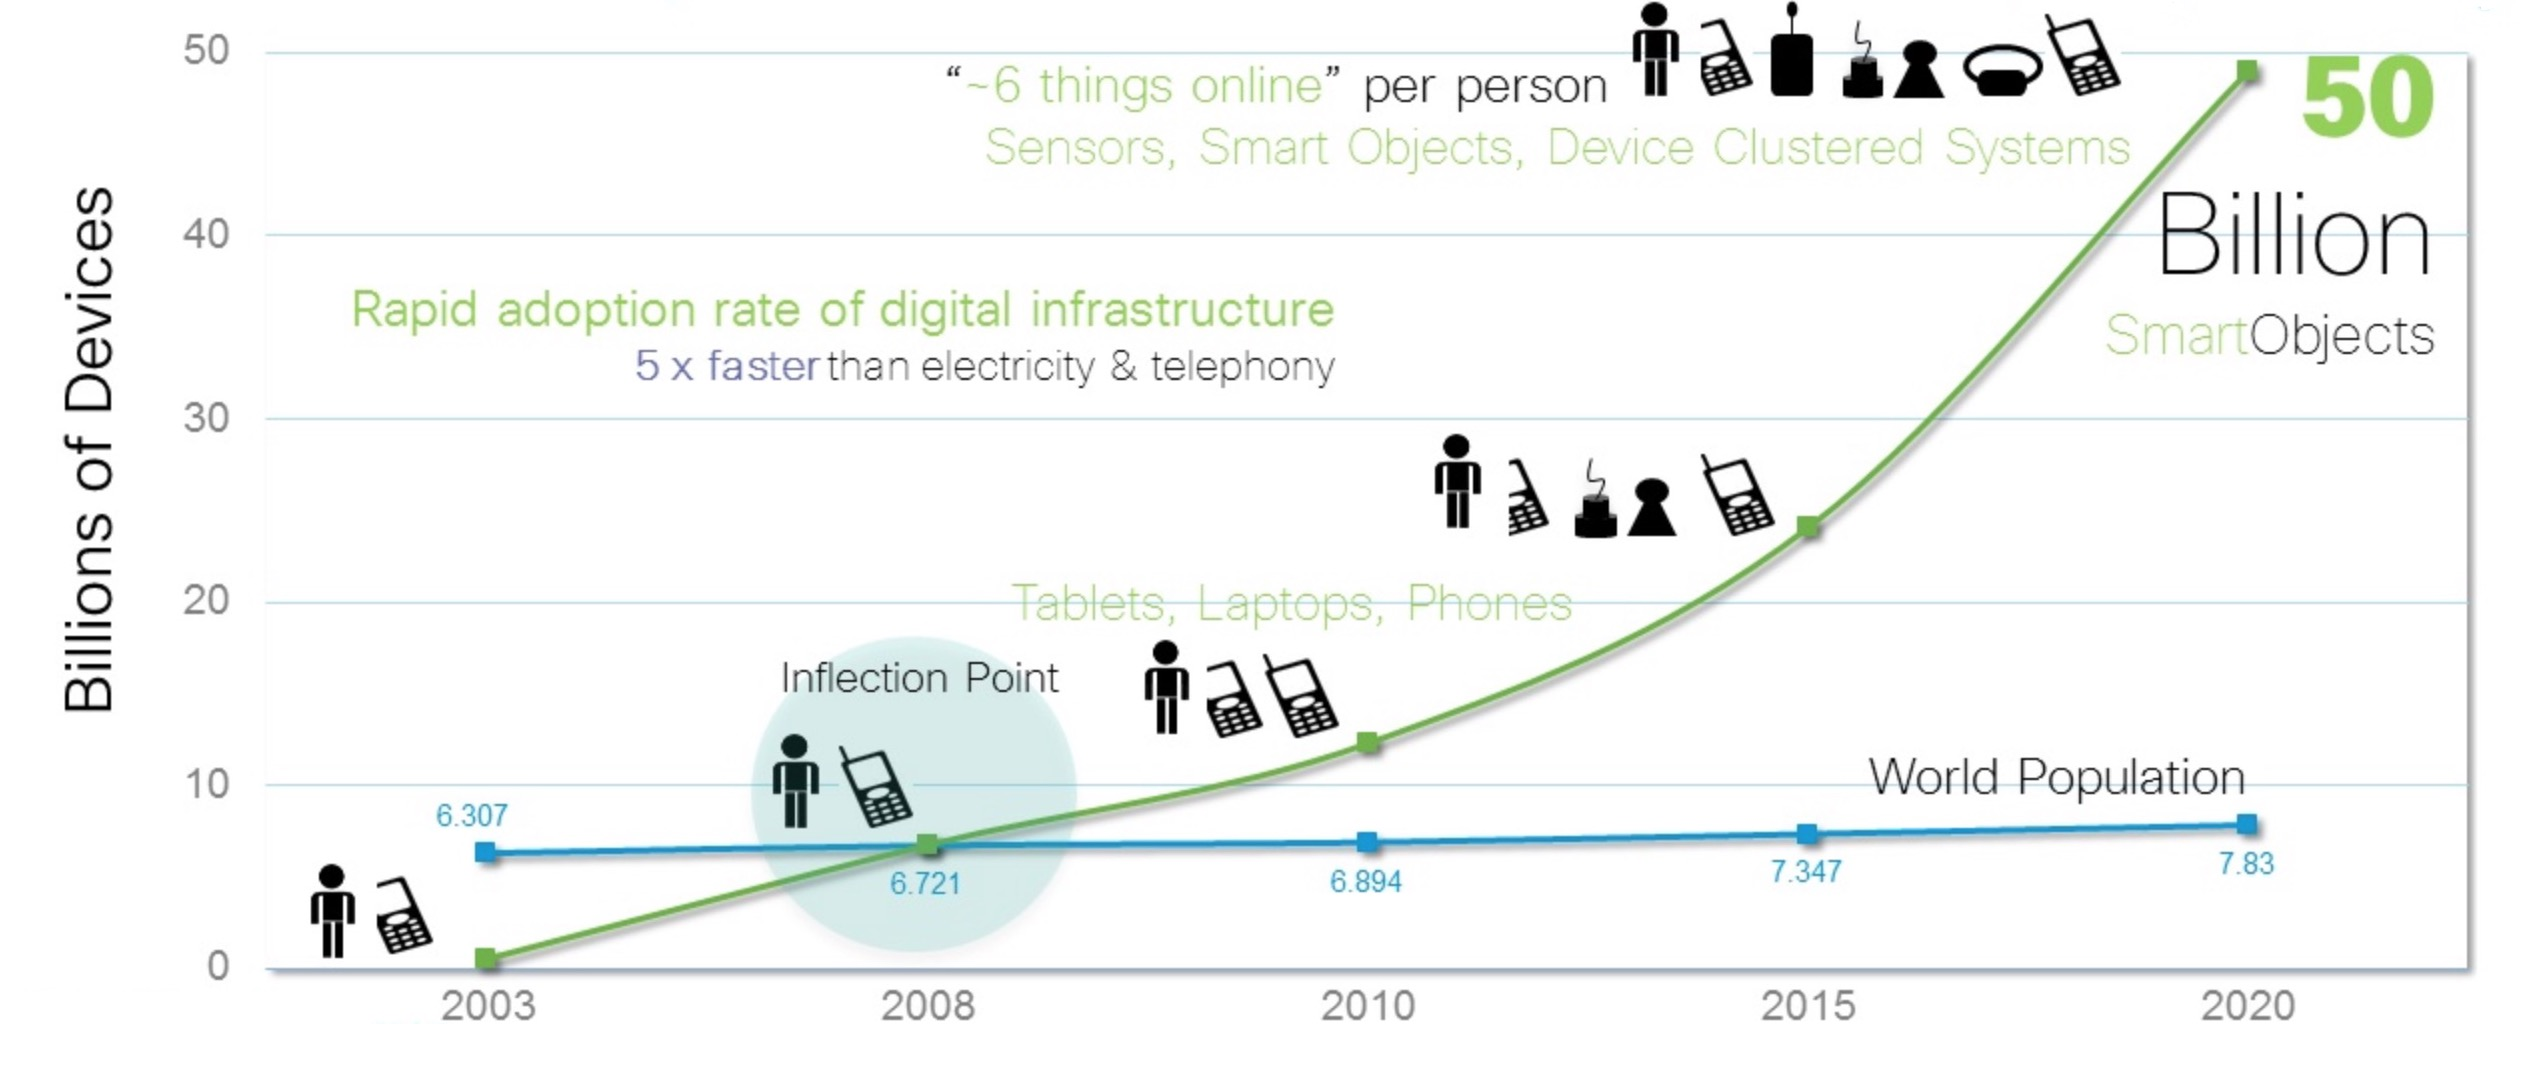
\includegraphics[width=12cm,height=6cm]{/Users/henninghakonsen/Dropbox/Masteroppgave/thesis/latex/images/popTo2300.jpg}
  \caption{\acrshort{iot} Growth \cite{online:IoT2020}}
  \label{pic:IoT2020}
\end{figure}

Currently we are at a point in time where it all comes down to how these \acrfull{lpwan} perform, which we will have a look at in this thesis. Up until now, \acrshort{iot} devices has communicated directly or indirectly with Internet, but in a rather complicated way. The typical scenario has been that the \acrfull{ue} communicate with a more complex device, often a wireless unit of some kind, and this device communicates with Internet over \acrshort{lte} or a wired connection. While this is an improvement and a step towards a future of connected things - the current mobile technology does not support the expected growth in this area.

The payload sent from \acrshort{iot} devices is usually small, typically 100bytes or less. However, the load of a \acrshort{lte} device on the current infrastructure, with all the signaling required, is too high. Hence, a simplified technology would allow less signaling and load on the telecoms infrastructure, while also enabling lowered monthly fees as a consequence. Price is always an important factor when choosing a new product. The typical cost of a mobile subscription with \acrshort{lte} and 5-10GB of data per month cost between 30€ and 50€, supporting 50-100 devices. The cost of a subscription over \acrshort{nb-iot} will according to Telenor and Q-Free be around 0.2€. In addition, hardware and installation costs are heavily reduced with \acrshort{nb-iot}. The aim is that an \acrshort{nb-iot} enabled device will cost around 60€. A similar \acrshort{lte} implementation would require a component that does \acrshort{lte} for embedded devices, which costs around 500€. A simple calculation[\ref{equation:ltevslwpa}] of the cost of 300 devices from a parking sensor use case shows that \acrshort{nb-iot} easily outperforms the current solution. TODO - verifisere utregning

Subscription: \label{equation:ltevslwpa}
Insert excel

In addition to lower cost, lower complexity there is a demand for increased coverage. Vehicles driving in vast areas, monitoring sensors position several meters under ground and devices located in packed cities are dependent of extreme coverage. \acrshort{nb-iot} will add 20 dB to the link margin, giving a huge coverage increase. This will enable such devices to operate while holding the power usage to a minimum.

Another motivator for \acrshort{iot} is the expected easiness of the setup. With todays technology you have to use sensors communicating over bluetooth or Wi-Fi to a common gateway which is connected to the Internet. With a \acrshort{nb-iot} device you will be able to connect directly to Internet, something many of us will be able to do without to much background experience. This will be an additional cause of growth in the number of \acrshort{iot} devices and is yet another reason why we need a new way of dealing with this technology.

The idea of some of the new \acrfull{lpwan} is to use the same hardware as \acrshort{lte} and add software to enable an \acrshort{iot} Platform. The most promising technology for sensor networks is \acrfull{nb-iot} and is enabled with a \acrshort{lte} core network as the bearing network. We will discuss how to implement \acrshort{nb-iot} in a \acrshort{lte} network in section, \vref{section:nb-iot-deployment}. This new technology should support an extreme amount of devices as well as them being in a secure environment. Security is a big concern when discussing \acrshort{iot} and we will elaborate on how this new network will provide security for the users in section, \vref{ssection:nb-iot-security}. Another concern is bandwidth and power consumption as mentioned. The bandwidth is reduced to a minimum and the power consumption is one of the main focuses. In section \ref{section:nb-iot-deployment} we will go into detail on this technology.

\section{Current status}
\subsection{Internet}
The main idea of the Internet we know today is quite similar to the past, but the scale and reach has outgrown what anyone thought could be achieved. In 2015 Google's data centers achieved high speed transfers up to 1 Petabit. "According to Vahdat, that is enough bandwidth for more than 100,000 servers to exchange data at 10 Gbps each, or transmit all scanned contents of the Library of Congress in under one-tenth of a second"\cite{online:petabitGoogle}. The reason for these data centers is the use of online resources. Offices, as well as home users require more bandwidth and reliability of the services provided from e.g. Google, VPNs, data storage and so forth.
Internet is everywhere and will continue to grow the coming years. As we will discuss in a later section we are seeing signs of a future where literally everything comes online. This includes wearables, industry monitoring and management systems and this will hopefully engage in a smarter and healthier society.

\subsection{Mobile networks}
Norway's GSM network came online in 1993 \cite{online:gsmTelenorNetcom} and Norway has pressured the current technology to reach higher standards from this time. The evolution of wireless radio technology has usually been focused on making it faster, while under prioritizing battery lifetime and simplicity. However, because this technology is used in mobile devices, it is for most users good news. \acrshort{lte} offers high \acrfull{ul} and \acrfull{dl} speeds and good coverage. One problem with \acrshort{lte} and older wireless technologies is that it consumes a lot of power. People are experiencing high speed transfers to their mobile devices, but at a cost draining their batteries. In the future, power efficiency has to be one of the main features of networks established. This is especially the case for sensor networks as these devices need to be connected to a mobile network. Such sensors are often established in remote locations without steady power. Using \acrshort{lte} or some other standard solution would give these devices short lifetime.

\subsection{A closer look at \acrshort{lte}} \label{ssection:lte}
\acrfull{lte} networks consists of some particular nodes for the network to connect to \acrfull{ue} and Internet. We call this structure \acrfull{epc} \cite{online:epc}. In this section we will get a better look at some of the attributes of \acrshort{lte} and the parts which make the \acrshort{epc} network. We really need to understand the underlying network to get a grasp of the new technologies we will investigate. Some of the standards we will mention are using proprietary solutions, but most of them are using \acrshort{lte} as the main infrastructure. \acrshort{lte} was introduced in release 8 of the \acrshort{3gpp} in 2008. In a summation by Ericsson they state some facts about \acrshort{lte} from the initial release. \acrshort{lte} from release 8 supported 100Mbps \acrshort{dl} and 50Mbps \acrshort{ul}(Not peak speeds), reduced latency(down to 10ms) and was cost-effective to set up. \cite{online:lteIntroduction} As of release 10 by \acrshort{3gpp}(year 2011) the speeds were at astonishing 1 Gbps \acrshort{dl} and 500Mbps \acrshort{ul}, however the network is not suited for low powered devices.


\acrshort{lte} is composed by 5 components which interact with each other. \acrshort{mme}, \acrshort{hss}, \acrshort{s-gw} and \acrshort{p-gw} constitutes \acrfull{epc}. See outline of \acrshort{lte} topology in figure \vref{online:lteTopology}.
\begin{figure}[ht]
  \centering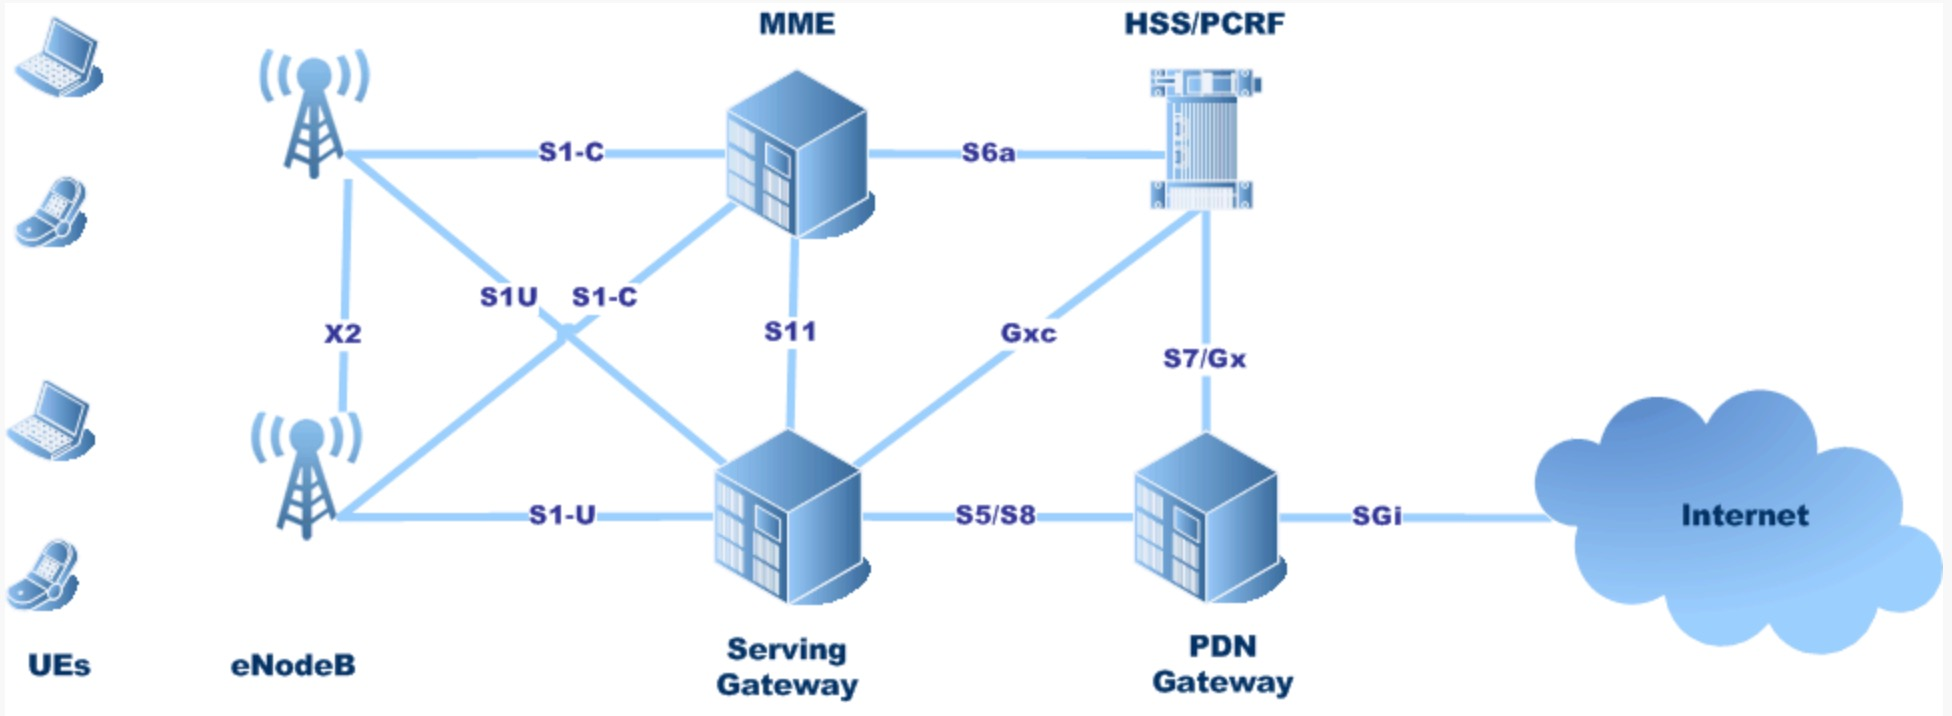
\includegraphics[width=12cm,height=6cm]{/Users/henninghakonsen/Dropbox/Masteroppgave/thesis/latex/images/epc.jpg}
  \caption{\acrlong{epc} \cite{online:lteTopology}}
  \label{online:lteTopology}
\end{figure}

\subsection{\acrshort{epc}}
%%http://www.3gpp.org/technologies/keywords-acronyms/100-the-evolved-packet-core
%%http://www.radio-electronics.com/info/cellulartelecomms/lte-long-term-evolution/sae-system-architecture-evolution-network.php

\subsubsection{\acrshort{mme}}
\acrfull{mme} is the main provider of signaling in \acrshort{lte}. \acrshort{mme} is connected to \acrshort{enb}, \acrshort{hss} and \acrshort{s-gw}, through S1-MME, S6 and S11 interfaces. It is in charge of authentication in cooperation with \acrshort{hss} which contains subscriber information, terminal-to-network negotiation and is a part of transition from LTE to 2G/3G.

\subsubsection{\acrshort{hss}}
\acrfull{hss} is the main database for information in the networks. It is a joint service originating from \acrfull{hlr} and \acrfull{auc}. \acrshort{hss} keeps information about subscriber information, that being user identification, addressing and profiles for a subscriber. Profiles describe how the network should perform for this special user and may include parameters like \acrshort{qos}(bandwidth and traffic class) and special modes, or states for a subscriber.
\newline
\acrshort{hss} also holds information about authentication between network and \acrshort{ue}s.

\subsubsection{\acrshort{s-gw} and \acrshort{p-gw}}
\acrfull{s-gw} and \acrfull{p-gw} deal with the user data plane and transports IP packets from \acrshort{epc} to external networks. The \acrshort{s-gw} maintains paths from \acrshort{enb}s to \acrshort{p-gw}s.

The \acrshort{p-gw} is responsible for the communication between the mobile intra network towards the Internet.

\section{Future - mobile networks} \label{section:futureapplications}
For the past ten years we have seen a rise in sensor activity. In the evolution of \acrshort{iot} devices, some has ported to \acrshort{lpwan}. However, as stated in the motivation, mobile \acrshort{iot} devices rely on good coverage and stability. Many people think of home electronics when discussing \acrshort{iot}, but this is not the main goal of \acrshort{iot}. Oslo's public transport operator(Ruter) has payment cards communicating with activation boxes over RFID, which in turn communicate with Internet. The Norwegian transport agency uses RFID in their tolling stations to communicate with cars. We also see smarter ways to implement these solutions. In the following sections we will give examples of application usage related to future mobile networks. In section \vref{ssection:wirelesstech} we will discuss how to approach technical solutions of future applications.

\subsection{Applications} \label{ssection:applications}
Sensors used for applications are not new. Already back in 2009 a forum called \acrfull{oecd} discussed ways to take advantage of sensors to support a green growth \cite{online:industryApplications}. This forum has members from all over the world, including Norway. The idea is that sensors can surveil and monitor emission numbers as well as act upon them. \acrshort{oecd} came up with a group of applications which were important to investigate. Some of them are smart grids and energy control systems, smart buildings, transport and logistics, agriculture and other general industrial applications. Together these fields combines most of the energy use today and with smarter systems we can reduce power consumption.

With this in mind we can clearly see that many of the fields \acrshort{oecd} discussed has been implemented, or is in the deployment stage. However the current status of industry activities related to these fields are running over 2G/3G networks. These networks provides good coverage while keeping the cost and energy low, but with billions of devices enrolling, this is not a sustainable model.

\acrfull{gsma} has made an overview of the most applicable areas of use. In figure \vref{pic:lpwan} some bullet points are presented for each area. In the next section we will comment special use cases for some of the areas.

\begin{figure}[ht]
  \centering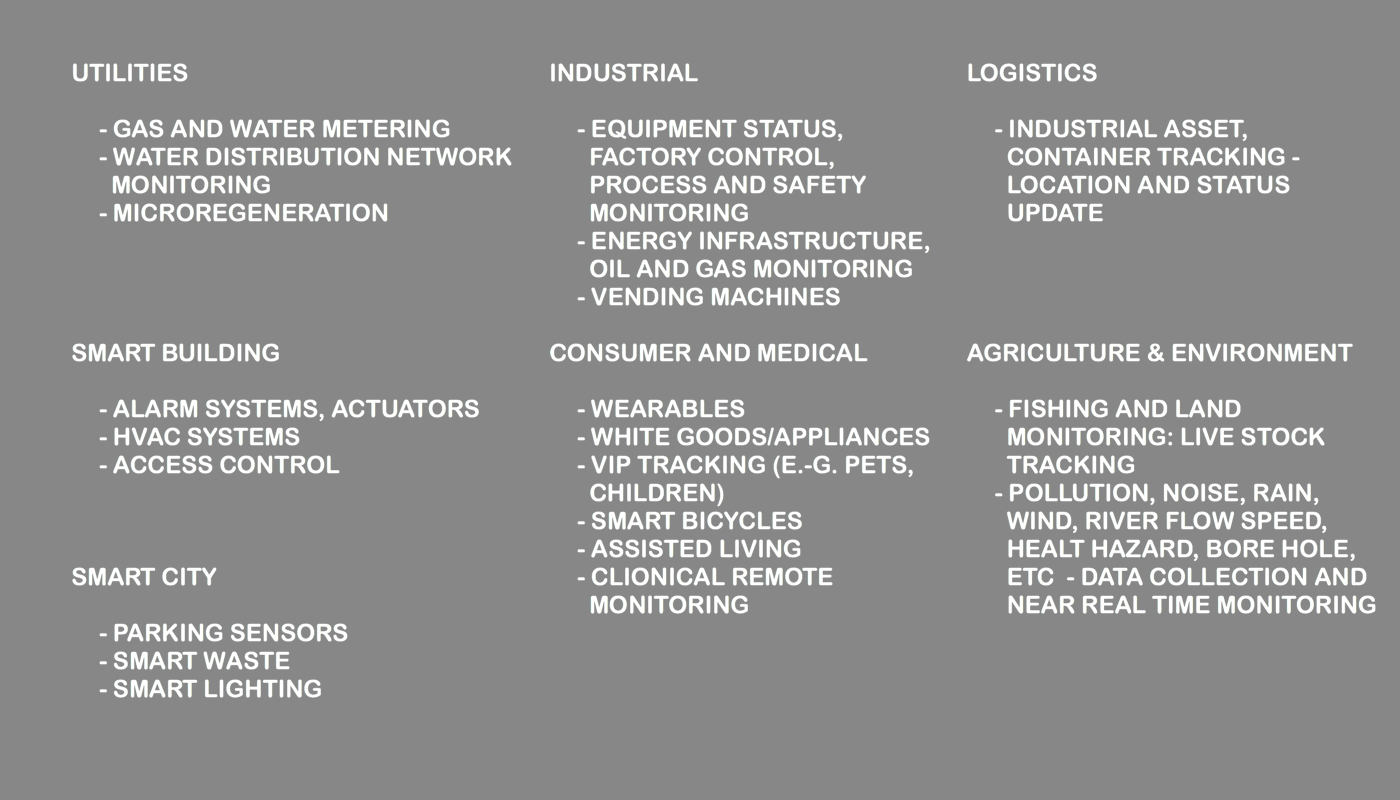
\includegraphics[width=12cm,height=6cm]{/Users/henninghakonsen/Dropbox/Masteroppgave/thesis/latex/images/lpwaArea.jpg}
  \caption{\acrshort{lpwan} example applications \cite{online:lpwaFuture}}
  \label{pic:lpwan}
\end{figure}

\subsubsection{Utilities and smart cities}
This domain resolves to what we are investigating in this thesis. Cities are getting smarter by the day and \acrshort{lpwan} can give us the stable network to deploy a large sensor network for monitoring and manage cities. \acrfull{its} is an initiative to control and manage traffic. The system provides communication between cars, trucks and sensors. The sensors are mounted in traffic lights, signs and other objects known in the transport field. The connected devices can adopt to the environment and help the society in several ways. Emergency units can set a route to an accident and the overlaying \acrshort{its} system will clear the way remotely to enable the emergency unit to quickly arrive at the location.

\paragraph{Parking - a realistic use case} \label{paragraph:sensoroutline}
Smart parking is a big investment point in big cities. Even though cars may be banned from the cities in some cities, parking at a nearby location can easier be managed with sensors communicating over \acrshort{lpwan}. Q-Free is mainly focusing on parking sensors related to \acrshort{nb-iot}. The sensor is housed in by a small plastic case which will be leveled with the ground. It withstands extreme forces and detects cars by magnetometer and pulsed Doppler radar. The housing is the most expensive part of the sensor, being able to withstand rough conditions for over 10 years. The idea is that the sensor is drilled into the ground, and will communication over \acrshort{nb-iot}. It will send status of the occupancy of the parking spot with a fixed interval, as well as reporting parking events when they occur. The growth of these types of sensors will increase and hopefully will they enrich our daily lives. See figure \ref{pic:parkingsensor} for a photo of the parking sensor from Q-Free.

\begin{figure}[ht]
  \centering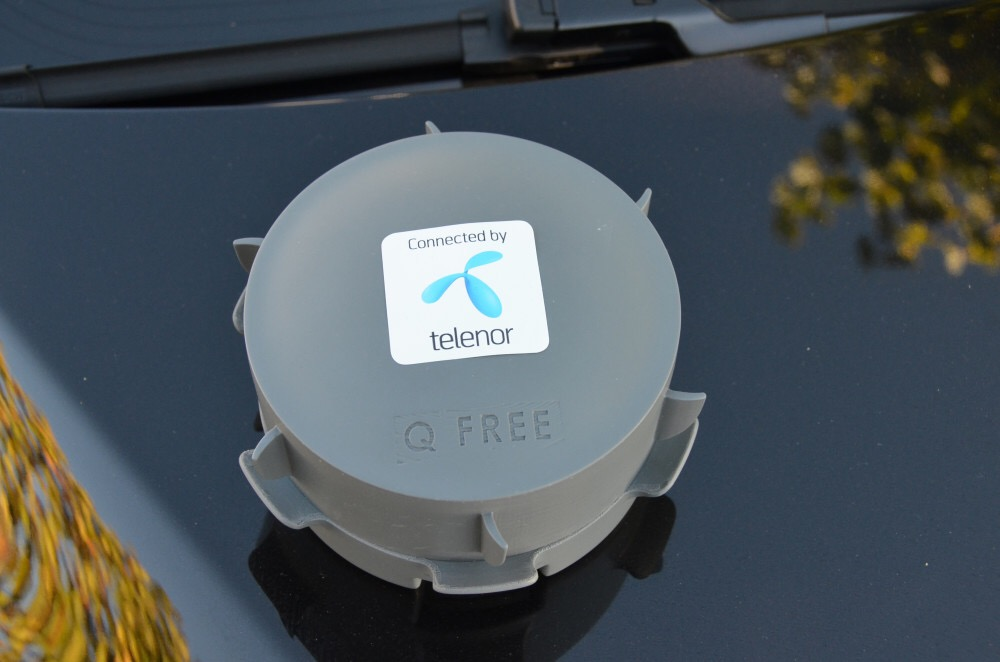
\includegraphics[width=12cm,height=8cm]{/Users/henninghakonsen/Dropbox/Masteroppgave/thesis/latex/images/parkingsensor.jpg}
  \caption{Parking sensor  \cite{person:ola}}
  \label{pic:parkingsensor}
\end{figure}

Other usage areas of sensors in cities are e.g. waste areas, power monitoring and \ce{CO2} monitoring. Operations can heavily benefit from more information, as well as automated procedures. There are many use cases where monitoring can be difficult and costly. With simple and cheap devices one could monitor hundreds of different things. As a result the work effort could decrease and the processes can be more efficient. A good example is garbage disposal. If garbage containers were fitted with measuring sensors, the control system can be notified when it is time to empty the garbage. The use case for this will probably be bigger companies and industrial sites, however it might be used for private residents as well.

These devices need to be cost efficient since they will be deployed in large scale. In 2014 a power supplier in Norway called Lyse began installing smart power meters in over 140 000 households \cite{online:lyseAMS}. These devices communicate with the mobile network in the area over a proprietary standard. While it is important to explore new solutions, this is one of many examples where standardized solutions will greatly outperform proprietary solutions.

\subsubsection{Logistics}
Today parcel tracking is a huge success and some companies are using sensors in their trucks and parcels for real time tracking. Using \acrshort{lpwan} networks will reduce cost of the devices and with long battery lifetime the sensors can be reused. In addition, the coverage for tracing the parcels will have to be great. However, for trucks it might be a better idea to wire the sensor to the trucks power outage. If you want real time, or near real time tracking, the sensor would have to send position data often and this will drain the battery substantially. There are some pros to use \acrshort{lpwan} networks for information collection, but this is probably not the biggest \acrshort{iot} area.

\subsubsection{Industrial}
Industry is a wide area and covers sites like gas stations, construction sites and factories. \acrshort{gsma} also includes vending machines in this category \cite{online:lpwaFuture}. With sensors communicating over \acrshort{lpwan} industry stations can be more automated and it is easier to surveil the systems. Downtime on such systems means lost revenue and efficiency. Low cost sensors which are wireless will hopefully have good coverage and uptime so that these systems run better. This is probably one of the areas where these sensors will be used more frequently since these systems needs realtime monitoring. Another problem solver \acrshort{lpwan} could be for industry use is the excellent coverage. As mentioned good coverage would prevent downtime, but it is also important to notice where some of these sensors will be placed. Factories, sub-sea and underground are some of the locations where industry is often located and therefore coverage is especially important for industry usage.

\subsubsection{Consumer}
Many people think of consumer products when talking about \acrshort{iot}. We are seeing growth in smart watches and smart wearables. The biggest problem with these devices today is the battery life and this is due to the extreme cost of communicating either with your mobile telephone over bluetooth or over \acrshort{lte}. It will be interesting when these watches will use \acrshort{lpwan}. Some wearables, such as your watch may use a standard with higher bandwidth than e.g. \acrshort{nb-iot}. For normal use, one would probably prefer \acrshort{catm} which offers bandwidth up to 1\acrshort{mbit} and could possibly provide music playback and phone calls.


Another interesting use case is smart homes. We have seen a move towards smarter homes for a long time, with better alarms, water and gas metering, light control and so forth. While this usually has communicated over Wi-Fi, there is a potential market where tradition Wi-Fi is not possible or preferable, and hence \acrshort{lpwan} can be used.

\subsubsection{Medical}
A potential step into a healthier society is for medical clinics to be able to monitor and give realtime consulting to their patients. The patients device could automatically uploaded real time data to their doctor, enabling them to uncover symptoms or deceases at an early stage and by this increase the average lifetime. One can also collect a lot of data for patients with a special decease and research for a cure. For this to be realistic we really need \acrshort{lpwan} since these sensors will have to be cheap and the stability has to be good.

In Norway we are going into an era where the number of elderly will increase heavily. We should seize the opportunity to use this technology to take care of the elderly. A person which needs attention, but can live alone, would prefer a device which communicates with the care center. The person could also raise an alarm with this system to alert the care takers. In this way the person will probably have a better life and the cost will stay lower.

\subsection{Developing wireless technologies} \label{ssection:wirelesstech}
\subsubsection{The general idea}
As mentioned in the motivation the general idea of new wireless technologies is to reuse the current infrastructure. The new networks will use some combination of \acrshort{lte} and all its components as discussed in section \vref{ssection:lte}. One may also use \acrshort{gsm}, as the current advantage of this network is that the coverage is better at the moment. In a couple of years \acrshort{lte} will be deployed all places GSM covers and we will probably see an increase in coverage as well. Coverage and power consumption are key features of developing wireless technologies and in combination with easiness it is the reason why some technologies stick while others fade away. Easiness is a requirement for \acrshort{lpwan} since the amount of data per packet is relatively small. For some of the technologies, guarantied delivery is not important, but it is important to acknowledge that we may need fast delivery for some applications which uses realtime monitoring.
\acrshort{nb-iot} will not suffice for these applications and we need to consider using technologies in parallel or speed up the transmission for e.g. \acrshort{nb-iot}. In the future this may not be a problem considering the pace of wireless evolution. Never the less it is important to not suppress this issue. We know from earlier research that if a user of a platform has to choose between multiple technologies the easiness of the platform impedes.

\subsubsection{eMTC/LTE-M and \acrshort{nb-iot}}
\acrfull{emtc} was standardized in the 12th release of \acrshort{3gpp} and updated with \acrshort{nb-iot} in the 13th release. It is meant as an high bandwidth alternative to \acrshort{nb-iot} and is often referred to as \acrshort{lte-m1}.

Both standards are implemented using the current \acrshort{lte} infrastructure, but they differ in coverage, bandwidth and the number of bands used in a cell tower. We see in figure \vref{figure:legacyWire} that \acrshort{lte-m1} provides bandwidth up to 1\acrshort{mbit} while \acrshort{nb-iot} peakes at around 200\acrshort{kbit}(rates from the release they were standardized). The coupling loss of \acrshort{lte-m1} is said to be around seven times better than \acrshort{lte}, and \acrshort{nb-iot} ten times better. We will cover the details about how \acrshort{nb-iot} uses the current infrastructure in section \vref{section:nb-iot}. \acrshort{lte-m1} can be used in the same matter.

\subsubsection{LoRa \cite{online:LoRa}}
\acrshort{lora} is the most popular non standard solution for enabling \acrshort{iot} devices. It is currently deployed in many cities and uses a proprietary solution. The devices which has a \acrshort{lora} chip uses RF or WiFi to communicate with a common gateway, typically a "cell" tower. The current range is up to 15km, but in dense areas the range only covers 2-5km. The bandwidth is low, but in light of the messages being passed to the gateway that is fine. In figure \vref{figure:LoRa} we see the overlaying infrastructure of a \acrshort{lora} network. It uses many of the same features as we mentioned in the motivation where the devices communicate with a middle box(concentrator/gateway), which in turn communicates with Internet over 3G or ethernet.

\begin{figure}[ht]
  \centering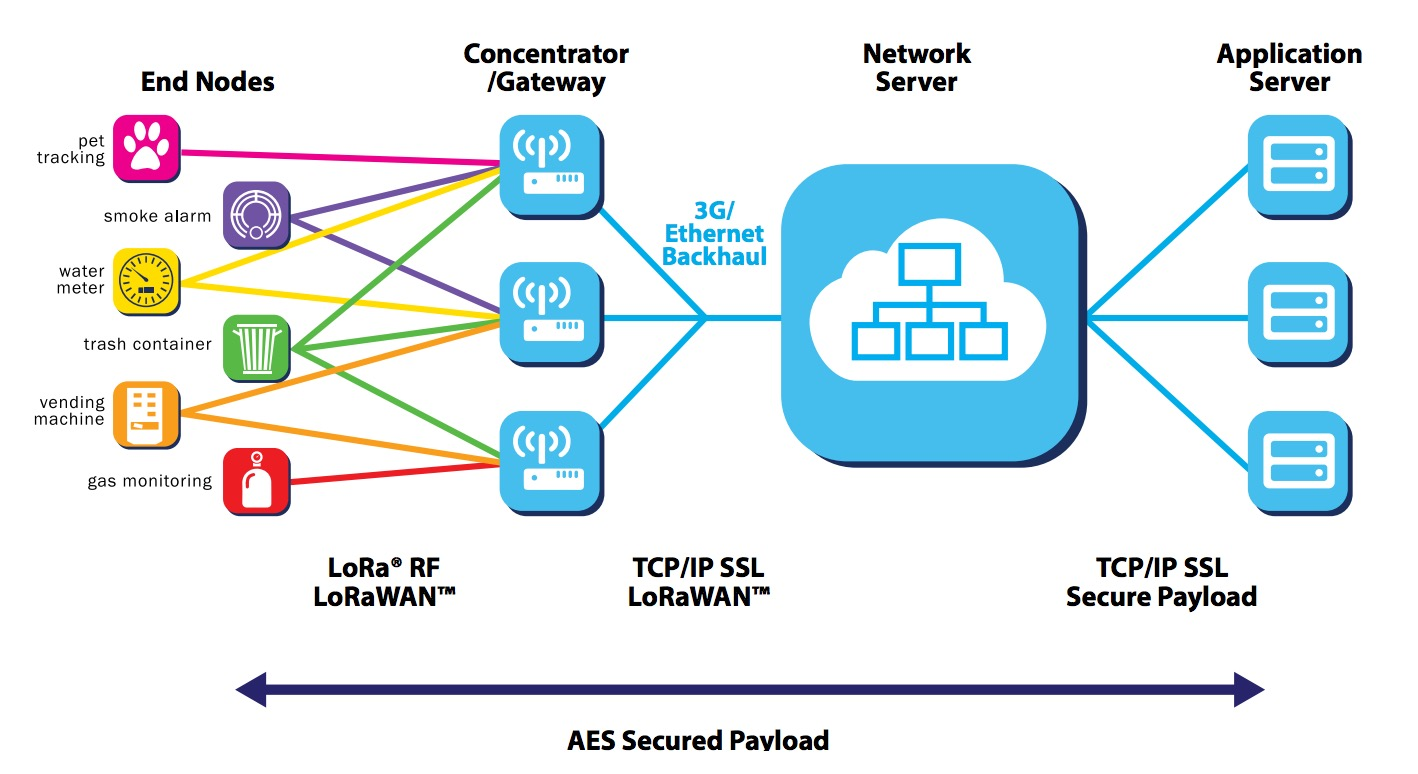
\includegraphics[width=12cm,height=6cm]{/Users/henninghakonsen/Dropbox/Masteroppgave/thesis/latex/images/lora.jpg}
  \caption{\acrshort{lora} infrastructure \cite{online:LoRa}}
  \label{figure:LoRa}
\end{figure}

The \acrshort{lora} solution provides an \acrshort{lpwan} at relatively low cost and gives average coverage compared to \acrshort{nb-iot} and \acrshort{lte-m1}. However, \acrshort{lte} is being deployed globally and if the coverage is good enough it will be more costly to provide \acrshort{lora} networks as well as \acrshort{nb-iot} or \acrshort{lte-m1} networks.

\begin{figure}[ht]
  \centering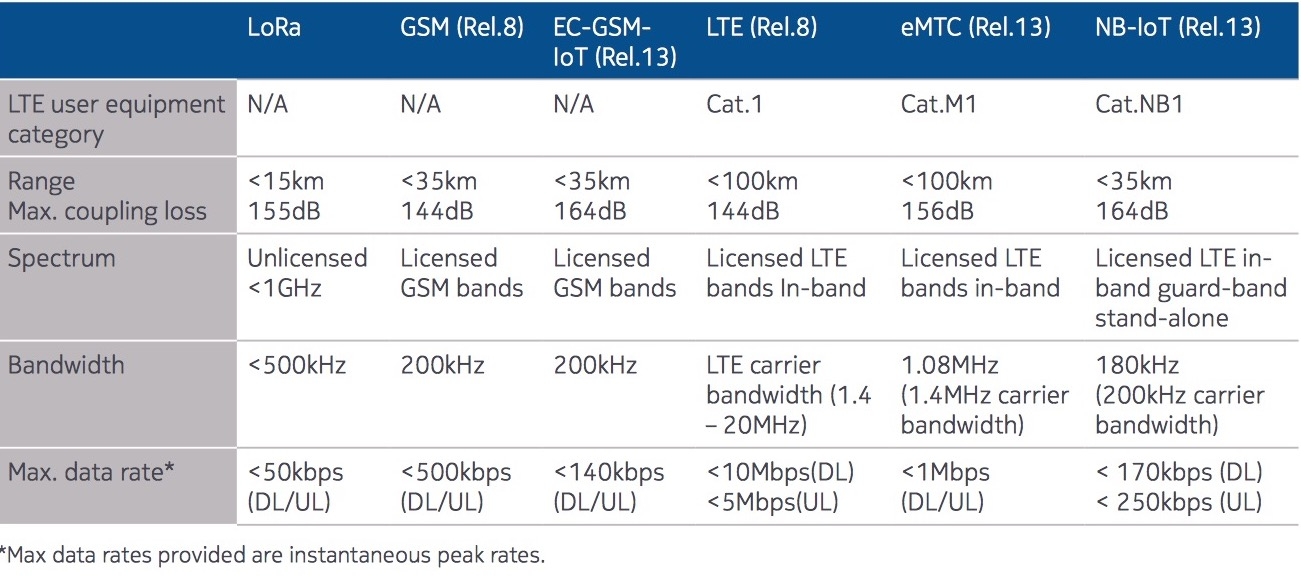
\includegraphics[width=12cm,height=6cm]{/Users/henninghakonsen/Dropbox/Masteroppgave/thesis/latex/images/lpwaKeyFeatures.jpg}
  \caption{\acrshort{lpwan} emerging solutions \cite{online:legacyWire}}
  \label{figure:legacyWire}
\end{figure}

\chapter{A dive into NarrowBand IoT} \label{section:nb-iot}
Telenor started their \acrshort{nb-iot} network test late 2016, with hardware mainly from Huawei. The goal of the test was to set up a \acrshort{nb-iot} network and test the communication with Q-Free's parking sensors, and run own tests before releasing the network to the public. They aim to launch their \acrshort{nb-iot} network in 2018 (HH)

We will focus on a general approach towards \acrshort{nb-iot} as technology and will test both Telenor and Telia's solution. In section, \vref{section:testing} we will discuss how and where we did the tests as well as giving you examples and results.

\acrfull{nb} \acrfull{iot} is the most promising \acrshort{lpwan} solution and the focusing technology in this thesis. The standard is made by \acrfull{3gpp} and \acrfull{etsi}, and was launched late summer of 2016 with the 13th release of the The Mobile Broadband Standard. The technology takes advantage of the current \acrshort{lte} infrastructure in a very sufficient way. The deployment requires no extra hardware, so the software necessary can be implemented into current hardware. In section \vref{section:nb-iot-deployment}, we will elaborate on the software required, as well as three ways to deploy \acrshort{nb-iot} in the frequency plan.

\section{System design}
In a system design process it is important to analyze the use of the new technology. It is crucial to understand how people and the industry will take use of \acrshort{nb-iot}. A good example of a standard which is causing problems today is \acrshort{ipv4}. When this standard was introduced, no one could predict the growth of online devices and for this reason \acrshort{nb-iot} has some specific system design features which hopefully will cover its use for foreseeable years ahead. In the next section we will briefly introduce the system requirements.

\begin{itemize}
  \item Link budget improvement \newline
  The sensors and devices in mind when deploying \acrshort{nb-iot} need better coverage than the average phone or \acrshort{lte} modem. As mentioned these sensors will be used in vast areas, underground and indoors. It is therefor important that the coverage is suited for this use. The goal is to reach 20dB extended coverage compared to \acrshort{lte}. Not only does this extend the range that these devices can be deployed, but they can emit transmissions with lower power, and hence use less power.

  \item Density \newline
  In the article from Cisco \cite{online:IoT2020}, they predict the growth of \acrshort{iot} devices. The prediction is that each household has on average 4 devices. According to Oslo council there are approximately 332 568 households per 1.1.2016 \cite{online:husholdningstatistikk}. This means that if we were to calculate the device pool today it would be around 1.3 million devices only for house holds. Taking into account that these devices will be broadly used by the industry as well, the device density will be very high. To put this into perspective we can investigate the device density of \acrshort{gsm}. For each \acrshort{gsm} cannel (200 KHz) there are 8 time slots, giving 8 concurrently connected devices. In one cell tower there are approximately 8 channels, and they are often split between mobile providers. If we assume that all of them belong to one provider, one cell tower can support up to 64 devices concurrently. One \acrshort{gsm} cell tower will provide coverage for the surrounding 1km, and since cell towers to close to each other will cause interference only one cell tower can provide coverage for 1km in radius. \acrshort{lte} has much more resources and can provide coverage for more devices, using time and wave division multiplexing.

  There is however a presumption to why \acrshort{nb-iot} can support so many devices per carrier. In the specifications one \acrshort{nb-iot} channel can support more than 50 thousand devices and keep in mind that \acrshort{nb-iot} can be deployed in one \acrshort{gsm} channel, which only supported 8 devices. The way this is supposed to work is due to the infrequent updates from the devices. One device might send a message every second hour and another might even send messages only once every day. One scenario where this might cause problems is if every programmer/company sends updates on specific times. Typically one would want updates at the hour marker(ie. 14:00, or 15:00). If thousands of devices do this at the same time, congestion and latency will definitively effect the experience for the devices.

  \item Low complexity \newline %%low cost
  A key feature for the devices supporting \acrshort{nb-iot} is that the complexity level is low. The new standard is less intricate than ordinary \acrshort{lte} which means that the devices can be less complex, resulting in cheaper hardware. This is an important factor for success since these devices need to be cheap to be broadly deployed. The complexity in this technology resides in the core mobile network for it to support many devices. Other than this, the technology supports average speed and average latency, perfect for monitoring purposes.

  \item Low power \newline
  The power consumption of the communication needed for \acrshort{lpwan} need to be low for the estimated battery lifetime of a device to be kept. The goal is over 10 years of lifetime, and since these devices probably will be very cheap, it might be cheaper to change the device instead of changing the battery.

  Low complexity and better coverage will help the device to consume less power, but it will not enable the device to operate for 10 years. The system design includes a special operation mode, called \acrlong{psm}. We will elaborate how this key feature will work in section \vref{ssection:psm}.

  \item Latency \newline
  For most applications applied to this new technology, latency is not key feature. We would like the device to send frequent, or infrequent message to a server or another device, but the time used is not important. However, what is actually a long time? A ping request on a normal wired connection today uses around 5-100ms, and even less for fiber connections. On mobile networks like \acrshort{lte}, the usual ping time is on average higher than on a wired connection, but usually it does not exceed 100ms. \acrshort{nb-iot} aims at a peak latency of 10 seconds. In comparison that is 100 times longer than a normal \acrshort{wan} connection, but it should suffice for most applications using \acrshort{lpwan}. The latency could probably be lowered, but it might interfere other design features, such as device density.

  \item Security \newline
  A big issue in Internet today is security, specially \acrshort{ddos} attacks. These attacks are more frequent and is an attack form which enables thousands of machines to continually spam one or several IP addresses, which in practice disables the application. In the fall of 2016, the DNS service provider "Dyn" was down because of a \acrshort{ddos} attack. Being a big DNS server, Dyn's downtime impacted major Internet platforms in both USA and Europe \cite{online:ddosAttack}. Since an attack like this needs a huge device pool it is likely to think that \acrshort{iot} devices are a potential tool for hackers. If hackers could access millions of devices with Internet access, they could easily perform global \acrshort{ddos} attacks which would halt our infrastructure, in turn disabling many of us to do our jobs.

  With this in mind, the engineers and designers of \acrshort{nb-iot} needed to consider security issues like this. We mentioned the \acrshort{iot} platform when discussing the deployment in section \ref{section:nb-iot-deployment}. This platform is the glue of \acrshort{nb-iot} and also a huge contributor of security measures in cooperation with \acrshort{mme} and \acrshort{hss}. The system requirement of \acrshort{nb-iot} is that no one should be able to directly access a \acrshort{nb-iot} device. One additional security feature in general with mobile networks is SIM cards. Like cell phones, \acrshort{nb-iot} devices will be fitted with a SIM card, which will enable the core network to authenticate the device, and visa versa. The SIM card has a subscription connected to the service provider, hence making a strong authentication scheme.
\end{itemize}

\section{Deployment} \label{section:nb-iot-deployment} %% HH legge til info om deployment i et LTE nett
In figure \vref{online:lteTopology} we saw the current infrastructure of \acrshort{lte}. To manage security issues and new features, a solution is to introduce a new term called \acrfull{iot-platform}. This platform will keep track of communication between outside applications and inside nodes. In theory the communication would suffice without this platform, but due to the extreme security issues regarding sensors we need a way to authenticate traffic. Many \acrshort{iot} devices are easy to hack and can be used for \acrfull{ddos} attacks. We have seen many service struggling with downtime due to overloading of their servers because of \acrshort{ddos} attacks. The platform ensures that traffic between two entities is secure, where one being the sensor and the other being the application server. For an application to receive traffic from a sensor, it will have to negotiate with the \acrshort{iot-platform} to gain access. After the setup procedure the \acrshort{iot-platform} acts as a \acrshort{nat} device, as well as matching correct application to correct user group, often called subscription. We might see other solutions for securing the internal network without negotiations.

\acrshort{iot-platform} is just one way to solve these issues. This software is in fact just an application proxy, or a firewall. Either way it can be implemented in the current hardware, but it is also possible to provide an extra rack mounted device to deal with this. In Telenor's test case, spring 2017, all the servers/hardware required was located at one location and the \acrshort{iot-platform} was running on private hardware from Huawei.

%% HH add section about the three states + graphs
\subsection{Operation modes}
\acrshort{nb-iot} occupies 180kHz bandwidth and there are currently three ways to integrate \acrshort{nb-iot} with \acrshort{lte}. The available operation modes are standalone, in-band and guard-band - see figure \vref{figure:nbiot-operationmodes} for illustrative definition. Standalone operation uses a dedicated GSM channel, utilizing the ability to deploy \acrshort{nb-iot} in \acrshort{gsm} as well as \acrshort{lte}. In figure \vref{figure:nbiot-operationmodes} we illustrate this operation mode to point out that \acrshort{nb-iot} can be deloyed in \acrshort{gsm}, even though this is not for the long run.

In-band operation utilizes bandwidth within one \acrshort{lte} carrier. This is the most technical and advanced solution and requires more work by the mobile network provider. The reason for this is because of interference between the \acrshort{lte} and \acrshort{nb-iot} sections in the carrier. It is worth noting that not all resource blocks within one carrier is available for \acrshort{nb-iot}. TODO verify??

Guard-band operation makes use of the bands not in use by \acrshort{lte} due to interference between \acrshort{lte} carriers. This in-between section is called a guard band and guards the carries for interfering with each other. This band can be used by \acrshort{nb-iot} and is a solution where one would want to utilize all resources of a cell tower.

\begin{figure}[ht]
  \centering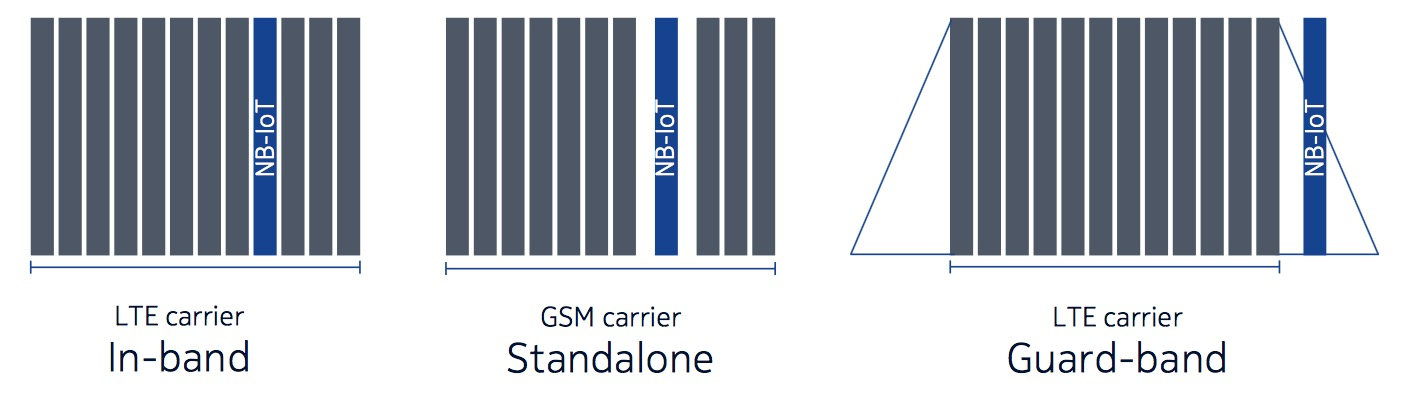
\includegraphics[width=12cm,height=4cm]{/Users/henninghakonsen/Dropbox/Masteroppgave/thesis/latex/images/nbiot-operationmodes.jpg}
  \caption{\acrshort{nb-iot} operation modes \cite{online:legacyWire}}
  \label{figure:nbiot-operationmodes}
\end{figure}

%%HH
\subsection{Security} \label{ssection:nb-iot-security}

\section{Introduction to energy saving} \label{section:energysaving}
Power saving is an important part of mobile communications for sensors. Several techniques are used to reduce power consumption, and \acrfull{drx} and \acrfull{psm} are two of them. \acrshort{drx} has existed for 20 years and is implemented in \acrshort{lte}, while \acrshort{psm} was introduced with the development of \acrshort{lpwan}. These two modes, together with paging\ref{ssection:paging} introduces an improved network, especially suited for sensors. In figure \vref{figure:nb-iot-timeconverge} you can see an outline of the communication process for a device. RRC Connected mode is the mode where the device actually can communicate with the network. The following procedures shows a possible time convergence graph for a device. We will explain the techniques used, as well as the specific time periods of the figure in the next sections.

\begin{figure}[ht]
  \centering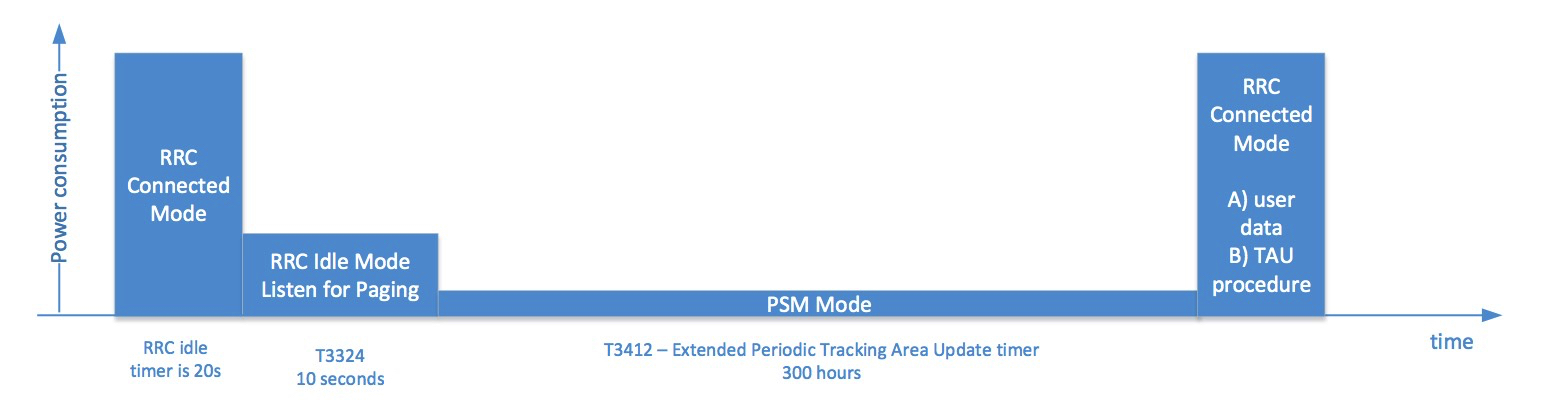
\includegraphics[width=12cm,height=6cm]{/Users/henninghakonsen/Dropbox/Masteroppgave/thesis/latex/images/nb-iot-timeconverge.jpg}
  \caption{\acrshort{nb-iot} time convergence \cite{person:ola}}
  \label{figure:nb-iot-timeconverge}
\end{figure}

\subparagraph{Prerequisites}
To get a good understanding of the results we need to closely look at the outcome of the results and understand the meaning. In the following sections will describe details about how \acrshort{nb-iot} works and what the specifications are saying. As stated we will be mostly focus our tests on coverage and power usage, which relates closely. Coverage is measured in \acrfull{dbm} and provides a relation between the distance between the base station and the \acrshort{ue}, and the transmit power of the \acrshort{ue}. In theory a device will transmit with the relative strength according to the coverage, so that the signal is received at the base station. Depending on the coverage of the device it will adjust the transmit power.

With this in mind we can convert coverage and transmit levels to output power. In worst case scenarios the device will transmit data with +23\acrshort{dbm}, which under normal circumstances is converted to 230\acrshort{ma} \cite{datasheet:ubloxchip}. We can convert \acrshort{dbm} to \acrshort{mw} by calculating 10\^(\acrshort{dbm} / 10). Keeping +23\acrshort{dbm} in mind gives us 10\^(23 / 10) = \~200\acrfull{mwh}. We can also convert from \acrshort{ma} to \acrshort{mwh} by multiplying \acrshort{ma} with the voltage, this gives us 0.230\acrfull{a} * 3.3V = 759 \acrshort{mwh}. The voltage into the chip is rated at 3.3V and we can assume that the spare power is used for keeping the device in connected mode which we will discuss later. HH

\acrshort{nb-iot} operates between -40 and +23\acrshort{dbm}, where -40\acrshort{dbm} equals 10\^(-4)=0.0001\acrshort{mwh} and +23\acrshort{dbm} equals 10\^(2.3)=200\acrshort{mwh}. We will see how this will influence the power usage in the tests and we will also touch on the subject in the following section.

\subsection{RRC connected mode} \label{ssection:rrc}
This mode is used when the device wants to communicate with the network, either \acrshort{ul} or \acrshort{dl}. The time spent in RRC connected mode can vary, but the default \acrshort{nb-iot} timer is 20 seconds. In this mode the device will use a lot more power, hence we want to move away from this mode as soon as we are finished transmitting or receiving data. When the chip is in active/connected mode it uses 6\acrshort{ma}=0.006\acrshort{a} * 3.3V =0.0000198\acrshort{mwh}.

When the transmit operation is finished the chip will stay in connected mode until the time period ends. There is an optional flag, "release assistance indicator", in the AT send command which puts the device into \acrshort{psm} directly after the transmit operation. The network needs to support this action to give the \acrshort{ue} permission to sleep. It is the network which decides what the \acrshort{ue} should do according to the network and the devices status. Given that the network supports release assistance indicator the battery life would be extended, since we only send data for a short period rather than waiting for downlink data which in many applications is not needed.

The calculated numbers in this section are based on specifications from the manual of the \acrshort{nb-iot} chip\cite{datasheet:ubloxchip}. We will try to test and verify these numbers in section, \vref{section:detailedtest}.

\subsection{RRC idle mode}
After ending RRC connected mode the device enters RRC idle mode listening for paging, using approximately 1mA. The default \acrshort{nb-iot} time is 10 seconds and in this mode the device can receive data from the network with a paging request, meaning that there is data for the device in the network. If there is more data in the network the device will re enter RRC connected mode and try to receive data from the network. If there is no more data for the device it can enter \acrshort{psm} or \acrshort{edrx}

\subsection{\acrfull{edrx}} \label{ssection:edrx}
\acrfull{drx} is a way in \acrshort{lte} to keep the device connected, but reducing the power usage by only checking for new data(paging) on time slots. After a sequence of communication the device goes into a \acrshort{drx} state where it periodically checks if the network has new information for the device. If there is information for the device, the device enters RRC connected mode where it can receive and send data. In the figure the \acrshort{drx} time(\acrfull{T3324}) is set to 10 seconds, after a period of 20 seconds in RRC idle mode.

When designing \acrshort{nb-iot}, \acrshort{drx} had to be implemented. However if the device always checks for paging the battery would decrease at a high rate. \acrshort{edrx} is therefor an outcome of the idea of \acrshort{drx} in the special case of sensor networks. It is a new way to handle communication for sensors which needs to wake up for certain events or messages from the network. In an article about \acrshort{edrx} and \acrshort{psm} for \acrshort{lte-m1} we find a great figure showing \acrshort{edrx} \vref{figure:edrx}. Even though this is for \acrshort{lte-m1} it applies for \acrshort{nb-iot} as well. After a device has communicated, either sending or receiving packets over the network, we want it to use as little power as possible. By default the device will enter \acrshort{drx} mode for a network-specified time and if configured go into \acrshort{psm} mode after the given time. As mentioned, for some applications we want the device to be able to receive packets without waking it self up.

The device will then go into \acrshort{edrx} instead of \acrshort{psm} mode. This means that for the most of the time the device will sleep, but periodically it will check for new information(paging). The period where the device sleeps is configurable in the network. Since the internal clocks in the devices often are unreliable, and the time between these syncs may be long(typically 1-2 hours), we need to first sync the clock and information between the device and the network. We call this operation sync guard. We have to do this due to communication based on time(time slots/\acrlong{tdma}). After this process the device will operate in normal \acrshort{drx} mode for a certain period(~10 seconds) and go to sleep after that period. This is a very power efficient way to keep the device more synchronized with the network, but it raises some practical problems. (either remove the last sentence or discuss it later). In the parking use case we only need to send information, hence we don't need to activate \acrshort{edrx} mode.

\begin{figure}[ht]
  \centering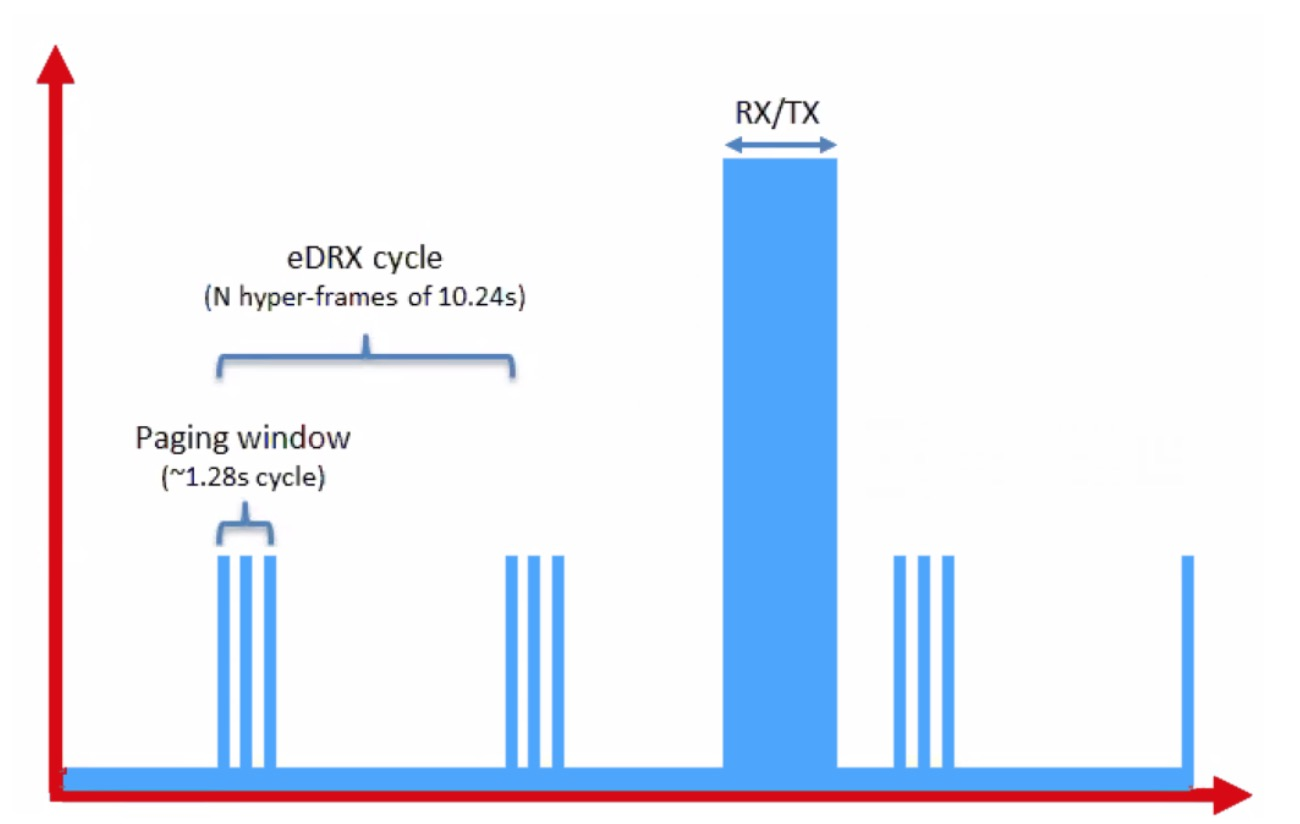
\includegraphics[width=12cm,height=6cm]{/Users/henninghakonsen/Dropbox/Masteroppgave/thesis/latex/images/edrx.jpg}
  \caption{\acrshort{edrx} operation mode \cite{online:edrxpsm}}
  \label{figure:edrx}
\end{figure}

\acrshort{edrx} has a set of configurable parameters which define how the \acrshort{ue} behave when entering \acrshort{edrx} mode. In short terms we want to specify \acrshort{edrx} cycle length and paging time window. The cycle length is the length of an \acrshort{edrx} cycle. This means the time from start of a period to the start of the next period. The cycle length can vary from 5 to 2621 seconds. The paging time window can be set to 0 to 20 seconds, where the value 0 means that paging is not in use. In section, \vref{ssection:paging}, we describe what paging is.

\subsection{\acrfull{psm}} \label{ssection:psm}
\acrshort{psm} is the core of power saving in \acrshort{nb-iot}, as well as many other \acrshort{lpwan}. The idea of almost all \acrshort{lpwan} is that the devices send information periodically, while sleeping 99\% the rest of the time. After a typical connected period we want to enter a sleeping mode where very little power is drawn, usually by an internal clock. This mode is called \acrshort{psm} and enables the device to sleep for a network configured time period. In our test case this time(\acrfull{T3412}) is set to 300 hours, almost two weeks. That means that the device will be removed from all meta data in the \acrshort{mme} after 300 hours if there is no communication. This technique is foremost for the devices which only sends information to a server. The way it works is that the device goes from connected mode, to \acrshort{drx} mode listening for information from the network. After this the device enters \acrshort{psm} mode if activated. When in \acrshort{psm} mode the only thing going on in the device is an internal clock which can start the system at a specific time. This is necessary since we want the device to wake up at a specific time and perform POST/SEND operations towards a server.

In \acrshort{psm} the chips power usage will be as low as 3$\mu$A, which is extremely low and the main reason why we can expect these types of sensors to achieve 10 years of battery lifetime.

%%http://www.link-labs.com/blog/lte-e-drx-psm-explained-for-lte-m1
\subsection{Paging} \label{ssection:paging}
Paging is a procedure to initiate communication from the network. If paging is enabled the \acrshort{ue} will listen for data from the network at given time intervals within a RRC idle or \acrshort{edrx} period. If the serve wants to communicate with the sensor it sends a message over the network and it will be stored at the IoT Platform until the device is paged in.

\subsection{ECL} \label{ssection:ecl}
As mentions in section, \vref{ssection:rrc}, the \acrshort{ue}s will enter different coverage modes based on their signal strength towards the base station. There are three levels of \acrfull{ecl}. At which coverage level devices switch over to the different levels is decided by the network. Telia uses -105\acrshort{dbm} for \acrshort{ecl}1 and -115\acrshort{dbm} for \acrshort{ecl}2 \cite{mail:teliaMailThread}, coverage better than this resolves to \acrshort{ecl}0. OML Telenor?

In \acrshort{ecl}0 the device will transmit the data once, and in level 1 and 2 the \acrshort{ue} will retransmit the data to ensure delivery of the packet.

\subsection{The transmit procedure}
We have looked at several techniques for \acrshort{nb-iot} and the specifications looks very good when the \acrshort{ue} has good coverage. In good coverage areas devices will transmit data with -40\acrshort{dbm}, with an average actual transmit time of ~200ms. However in worst case situations, the sensor will boost the signal up to +23\acrshort{dbm}, which in terms of power usage is two million times as high - (10\^2,3) / (10\^-4) = ~2 000 000. In addition, as stated, a sensor with bad reception will try to retransmit data. Depending on the coverage the device will enter different coverage modes, described in section \vref{ssection:ecl}. Given that the sensor has bad coverage, and is operating in \acrshort{ecl}2 mode the transmit time might be as long as 5 seconds for a single data transmit. The actual power usage increases rapidly and the chip would use 200\acrshort{mw} for as long as 5 seconds, resulting in a power usage of 200\acrshort{mw}*5S=1000\acrshort{mws}, which actually is 50 million times increase in power usage compared to optimal conditions. However, as we will see in our tests, -40\acrshort{dbm} is normally not possible to achieve.

In the following figure, \vref{figure:ecl_dbm}, is an outline of how the device chooses \acrshort{ecl} mode dependent on the signal quality. In theory the device should lower its transmit power equally to the signal strength. The graph represent the theory behind the adjustment of the transmit power and you will see how this actually works in section, \vref{section:testing}.

%%https://cdn.rohde-schwarz.com/pws/dl_downloads/dl_application/application_notes/1ma266/1MA266_0e_NB_IoT.pdf

\begin{figure}[ht]
  \centering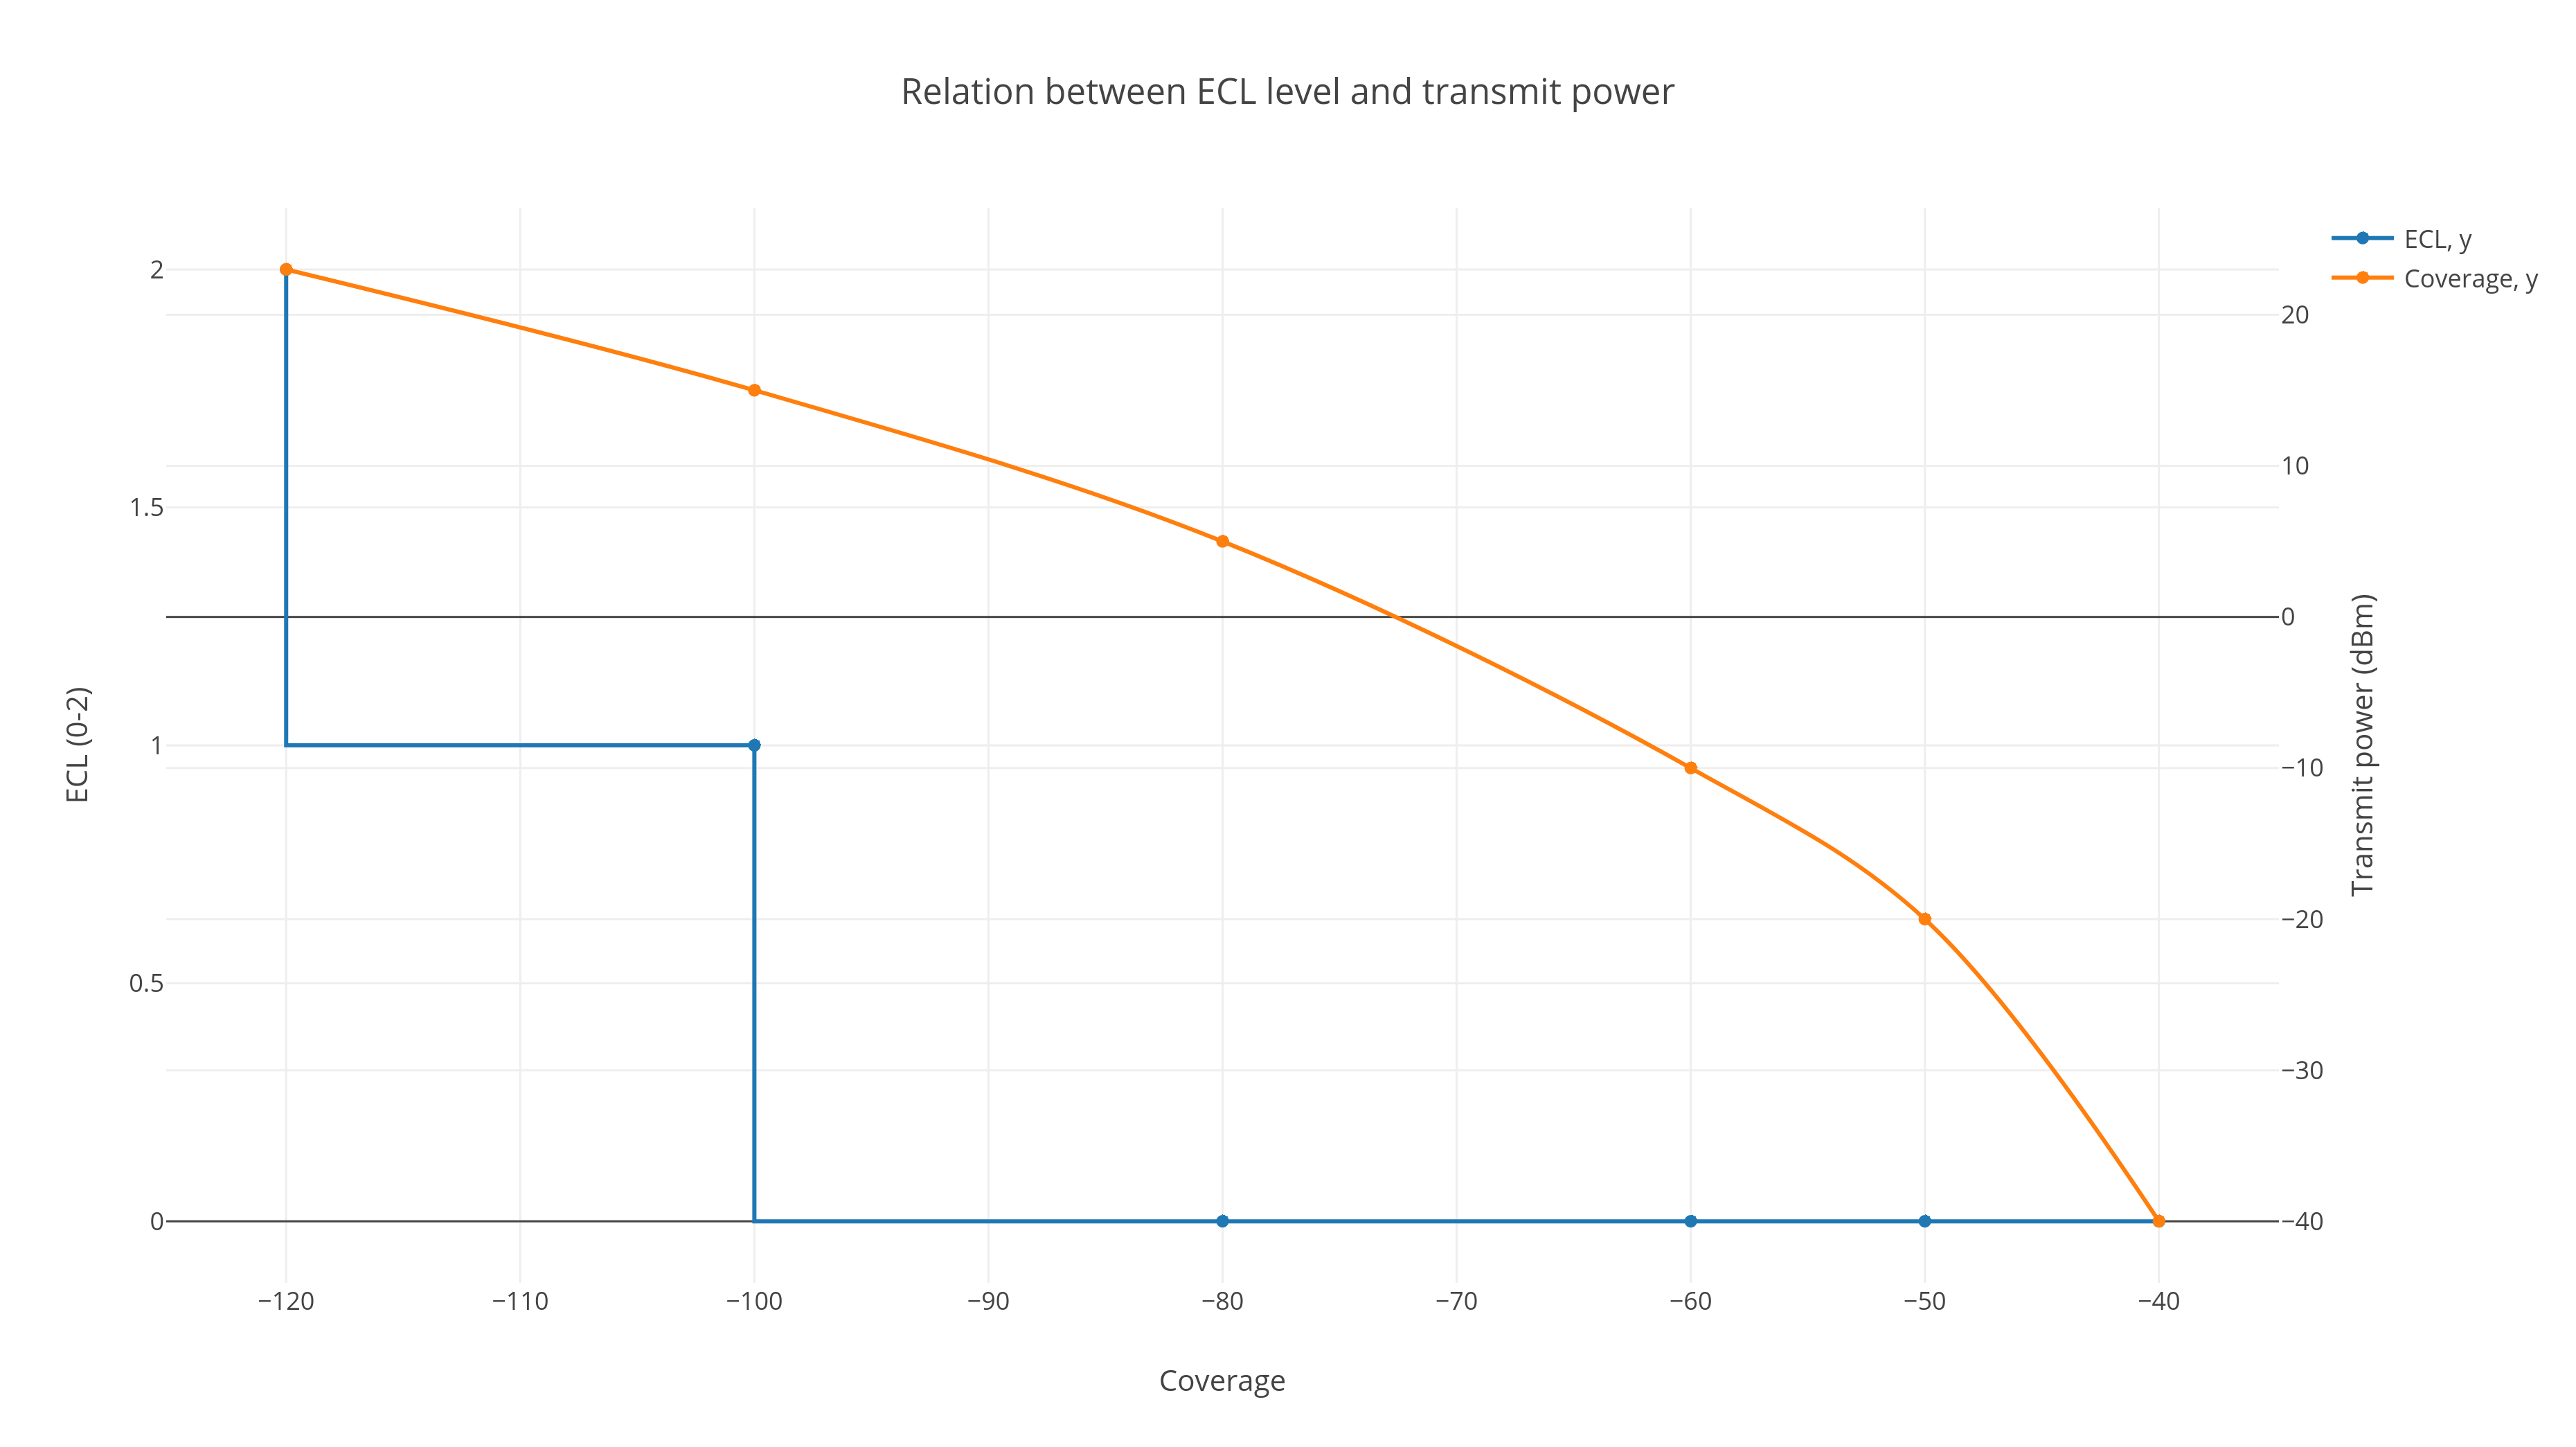
\includegraphics[width=12cm,height=8cm]{/Users/henninghakonsen/Dropbox/Masteroppgave/thesis/latex/images/ecl_tx_power_relation.png}
  \caption{\acrshort{ecl} and \acrshort{dbm}}
  \label{figure:ecl_dbm}
\end{figure}

\section{Parking - outline of the communication}
Parking is a huge market and therefore a great way to test both the coverage and practical use of \acrshort{nb-iot}. As of 2016 the parking sensors communicates to a common gateway(\acrshort{lte} embedded device), a device which communicates with the sensors using a proprietary narrowband communication technology in the ISM band, and to the Internet over \acrshort{lte}. This works fine, but as you might realized, the cost of the devices themselves and managing them are lowered significantly with \acrshort{lpwan} like \acrshort{nb-iot}. Q-Free has chosen to go with \acrshort{nb-iot} since this is the most promising technology providing the necessary specifications for their application. The communication between the sensor and the server is outlined in figure \vref{pic:sensorcommunication}. The sensor will send uplink messages every time there is a change to the parking spot or every half hour, or another configured time period. The sensor sends data to the eNB which in turn sends the data to the \acrshort{iot} platform. If a server has been authenticated within the platform the message is sent to the server. The server receives the packet and can display the message however it is necessary.

\begin{figure}[ht]
  \centering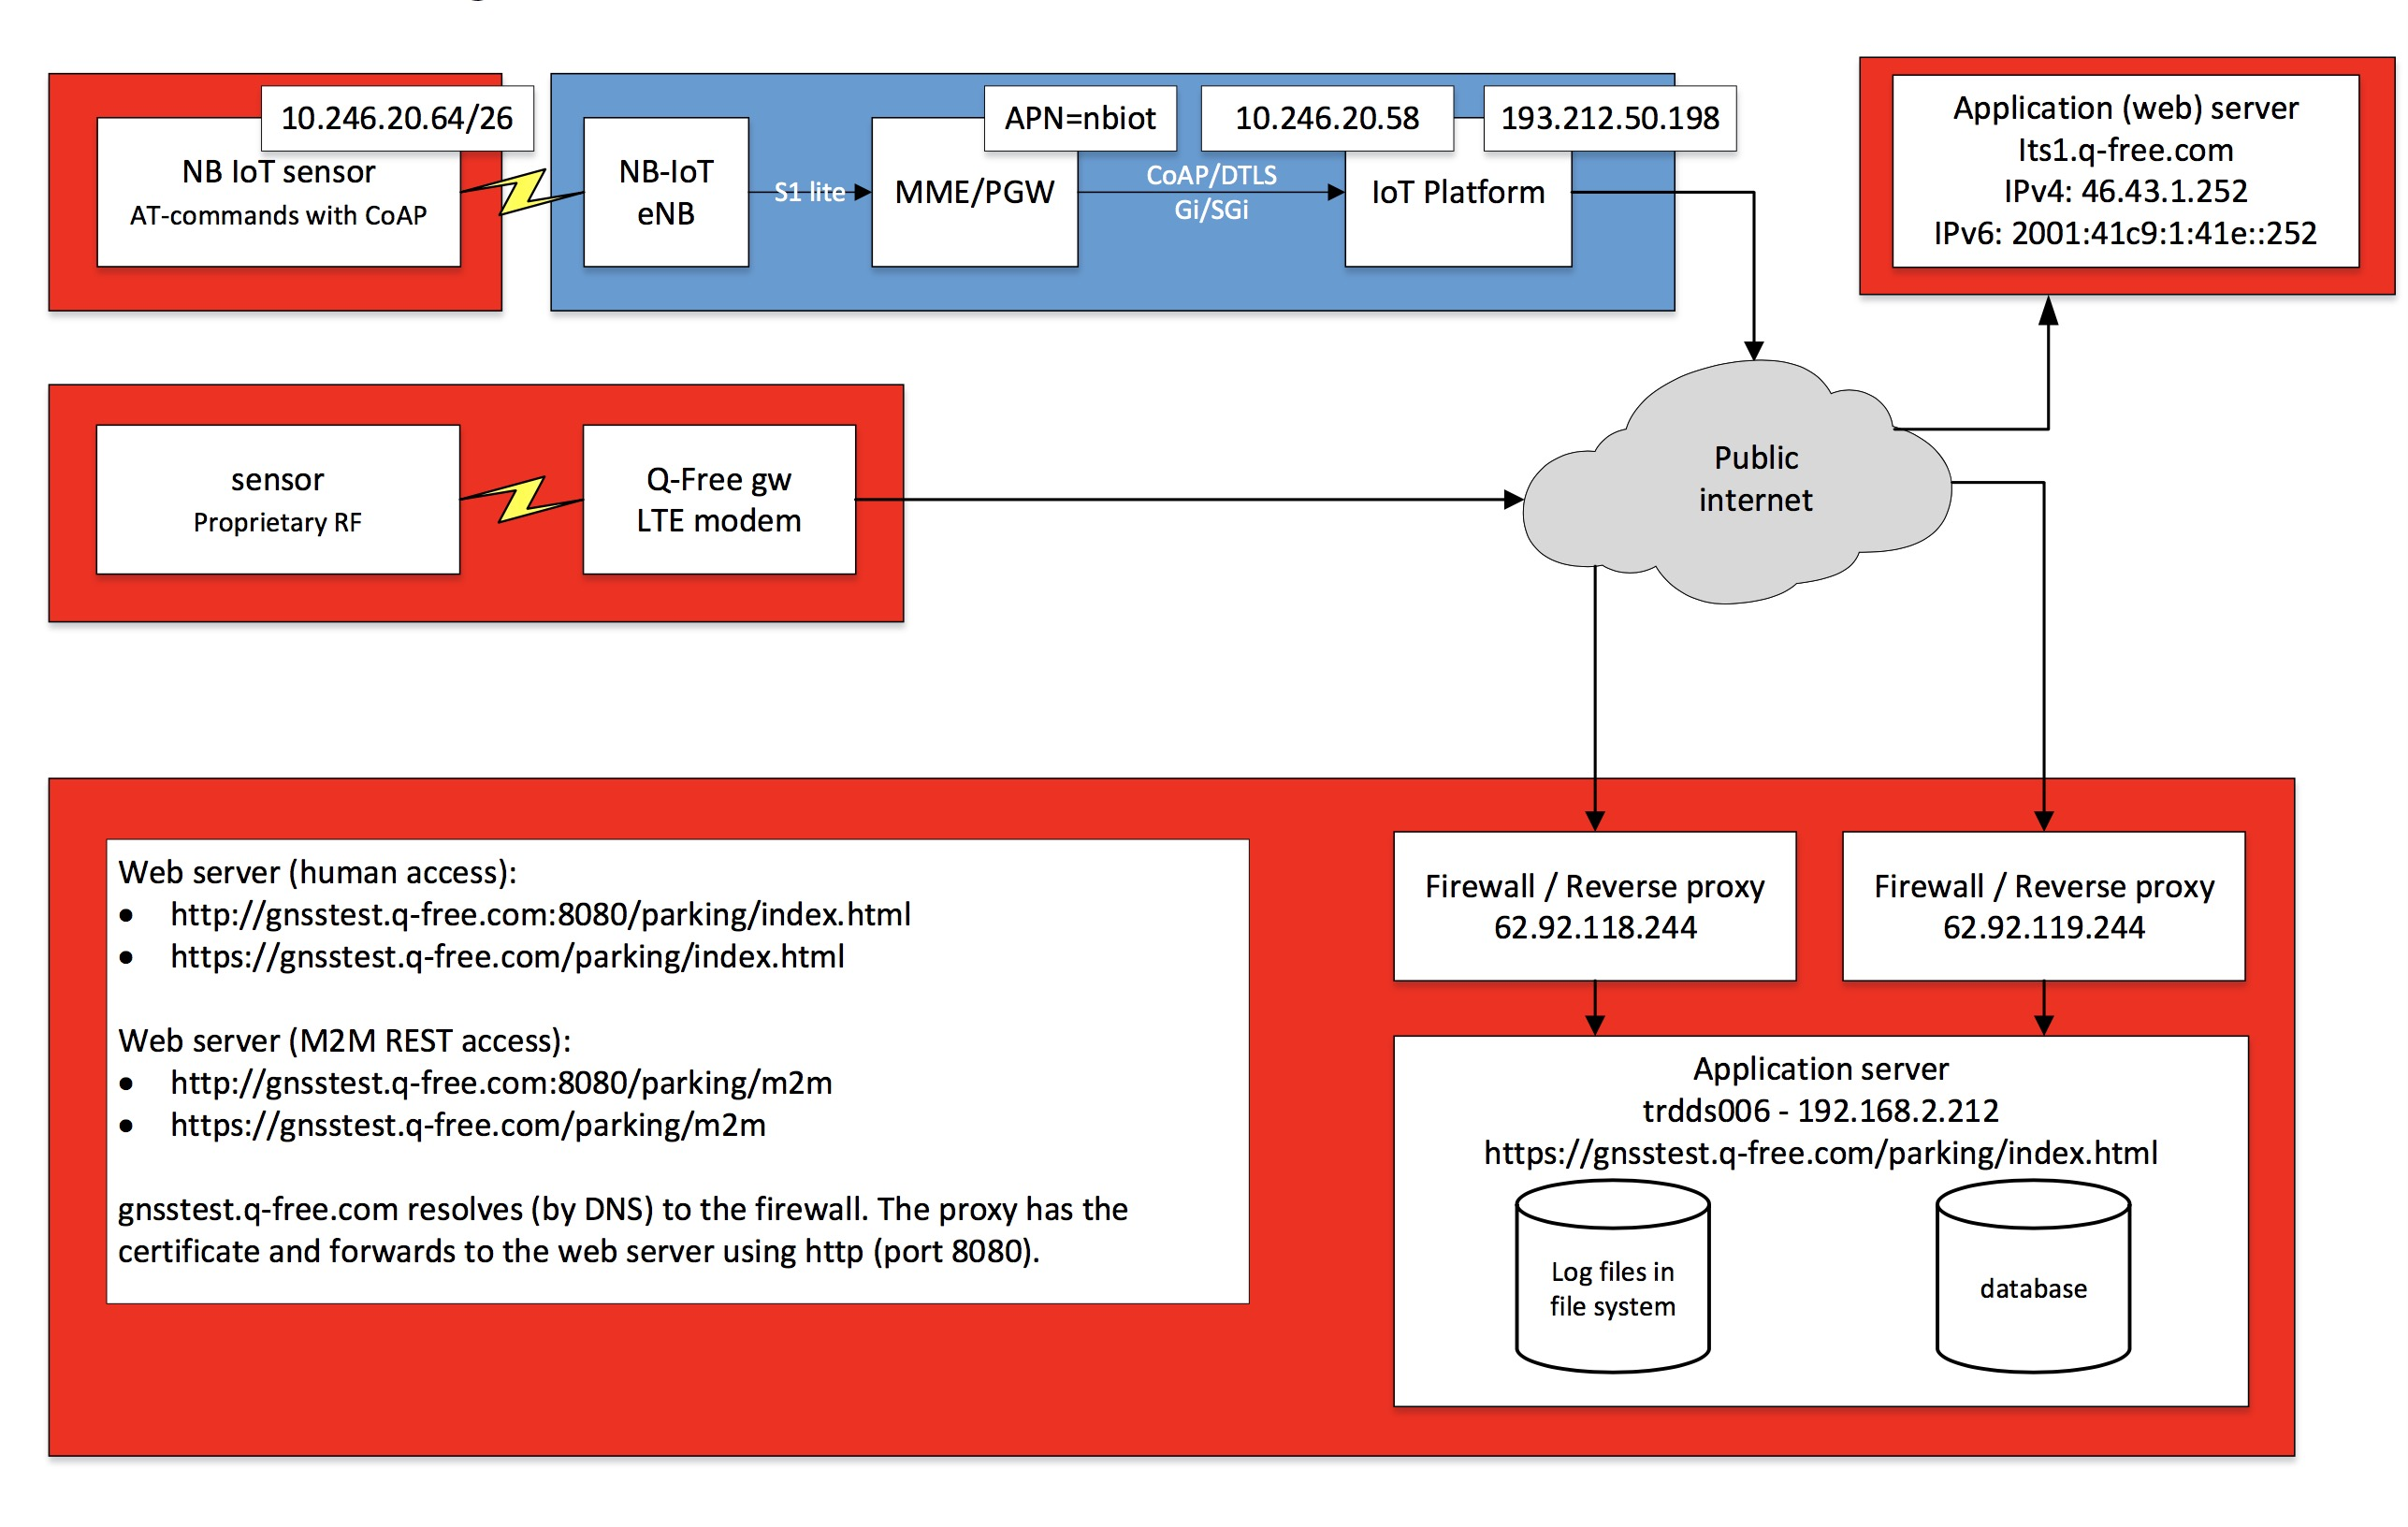
\includegraphics[width=12cm,height=8cm]{/Users/henninghakonsen/Dropbox/Masteroppgave/thesis/latex/images/sensorcommunication.jpg}
  \caption{Outline of sensor communication \cite{person:ola}}
  \label{pic:sensorcommunication}
\end{figure}

In this setup, the sensor is the one sending data to the server. One could also implement it the other way around. If each parking spot had a sensor with an ID of some sort. Then the car could extract the ID and send a message about parking at that particular parking spot. This might enable several parking operators to cooperate over a general infrastructure. %%HH privacy complications?

\section{Challenges}
%%HH change first line
what if the network fails?
power outage?
what should the application do if the sensor wont send?
how long should the sensor wait until doing anything?


With new standards there are always complications and challenges. One challenge in particular is the amount of communication between \acrshort{ue}s and the network. Say that your application needs to communicate every minute and the producer wants to use \acrshort{nb-iot}. The implementation will work, but might not be the optimal solution.

Another challenge for software developers and power usage is that some \acrshort{ue}s connected to \acrshort{nb-iot} will be online for a decade. This means changes in the network and possible power outages, which implies that the sensor has to cope with network changes and downtime in the network. Each time the sensor has to wake up and search for network the power usage increases and the lifetime of the sensor decreases. See section, \vref{ssection:downtimetest}, for tests.

%%HH rewrite
And consider the parking use case. Imagine a parking lot at a football arena, maybe in conjunction with a shopping mall. For most of the time the devices will send period messages when people are shopping and the sensors close to the main entrance will of course send messages more often then the ones long away. At the same time when a match is about to start the parking lot will be full instantaneous. This raises a particular question, how will the network cope with so many devices sending data close to each other. The number of devices activated in that particular area will be increased in a short time which may cause congestion and incorrect updates as \acrshort{nb-iot} is not fast or "reliable" in the sense that the data can be lost or delayed. The network may cope with these problems just fine, however it is worth considering these problems.


Even though parking could raise congestion problems, the flow of cars to a parking lot is limited. All parking spaces will not be filled at the same time. However, for water, electricity or other measuring procedures the sensors might be configured to send data at the same time. Take electricity measurement as an example. According to wikipedia \cite{online:avgpeople} there are approximately 5 000 residents per square kilometer in Oslo. In the city center this number is probably a bit higher as well. With this in mind one cell tower will provide coverage for around 2-3 thousand house holds and their electricity measuring device. If all of these devices sends updates at the same time, as well as other traffic is incoming, the network might be overloaded.

We will try to test these types of edge cases to see whether \acrshort{nb-iot} can handle difficult scenarios or if these applications would have to use a different technology.

\part{The project}
\chapter{Planning the project}
To get accurate and meaningful results we had a long planning phase. First of all we needed to decide how and what to test. We decided to set up a server, which can receive data from a \acrshort{nb-iot} chip. In addition, this server will be able to analyze the data and display the results in a meaningful way. We also needed a way to send data over \acrshort{nb-iot} to the to the server. We were so lucky to borrow a development kit for \acrshort{nb-iot} from Q-Free which enabled us to connect to the network. We also borrowed a SIM-card from Q-Free which used Telenor network. We also managed to get a SIM-card from Telia so that we could try to do some comparison between the two network providers. In section, \vref{section:detailedtest}, we will go into further detail about how the setup was and why we did the different tests.

With this in mind, we will describe and give you an introduction to the different parts of the setup and show you how they are tied together.


\section{The web application}
In order to collect data we needed a web server and we needed to consider a few things, what should be included in the server, which platform should the server run on and where should the server be located. At the same time it was important to think about how the data would be used. The simple solution would be to collect the data and import it into an excel document for analysis. However, the amount of data is big - in fact the db consists of XXX (HH) GB of data with over XXX elements. Rendering this in an excel document would not suffice for an effective analyzation of the data after the test. We decided to implement a web app to display information about the sensors. This web app can display uptime, latency and coverage data about each sensor as well as displaying average of all of them. In this way it is easy to view the data and draw conclusions.

In the following sections we will discuss the implementation of the server and the web app.

\subsection{Backend: Node.js}
We decided to use node.js for what would become the backend of the server. Node.js is a new and modern way to create simple REST APIs. A REST API follows a set of rules to make it robust and stateless. It also should include all CRUD operations(create, read, update and delete) and should use the appropriate request method, such as POST, GET, PUT and DELETE. A big difference from standard backend programming is that Node.js uses javascript as programming language. Even though javascript is not the cleanest programming language it is efficient and the codebase is kept low. In addition node.js takes advantage of using \acrfull{npm}. \acrshort{npm} offers packages for all applications, both frontend and backend, and we will discuss some of the packages used in the server.

The server hosts multiple API endpoints. The most important are of course collecting data and retrieving data. The database contains a lot of data collected from different tests and it would require a lot of rendering to do analysis on the client side. We decided to analyze the data at specific intervals so that the client would simple display the data. We will describe the analysis and data which is displayed in section, \vref{ssection:analysis}.

\subsubsection{The database}
There are multiple ways to store data and there is always a trade off when choosing the platform. PostgreSQL is a great example of a database which is fast and reliable, but it can be complicated to set up and is SQL driven which means all data has to fit into one or several tables. Since this project is small and the data is be represented in a couple (HH describe in "the project") of different ways we have chosen to use a NoSQL database. There are many good tools for storing data in a NoSQL database. ArangoDB and MongoDB are the most commonly used databases and both works well with Node.js. ArangoDB is often used for geo specific tasks and mongoDB was a bit easier to use, so we decided to use mongoDB for our data storage. In paragraph, \vref{subparagraph:mongodb}, we will explain how we used mongoDB for our implementation.

\subsubsection{\acrlong{npm}}

\subsubsection{Express}
Express is a fast and robust package for handling routes and offers nice APIs for listening on specific ports and so forth. In the following code example, \vref{code:express}, you can see the base setup for making your server handle requests. The port is set with a combination of the processes port and user specific port selection. The reason why this might be useful is if your server is hosted on a payed server which might be deployed on different IP and port for each deploy. With this implementation you won't need to consider this. In the example you can see a GET for a specific path, however you can also redirect all routes to a separate file for cleaner code. The last thing we need to do is to listen for incoming requests on the specific port. Now express will handle all request with an event loop.

\begin{lstlisting}[caption={Base express setup},label={code:express},language=JavaScript]
// express setup
const server = express();
const port = process.env.PORT || 8020;

server.get('/', function (req, res) {
  res.send('Hello World')
})

server.listen(port, () => {
  console.log(`app started on`, port);
});
\end{lstlisting}

\subparagraph{Coap}
Coap is a simple network protocol and offers request like HTTP, but without all the overhead. Coap is designed for low powered devices and will be used for our tests. I have used node-coap package for including coap support on the server. Since the protocol is simple, we need to handle the request a bit different. The following code example, \vref{code:coap}, shows a simple node-coap setup.

\begin{lstlisting}[caption={Base coap setup},label={code:coap},language=JavaScript]
var coap = require('coap')
var coap_server = coap.createServer()

coap_server.listen(port, () => {
    logger.log("info", `Worker ${process.pid} started coap server on ` + port);
})

// All request is handled by this function. It is not possible to request a specific url path
coap_server.on('request', function(req, res) {
    // Payload of the request is a byte stream. Parse the stream and handle the data
    var data = JSON.parse(req.payload.toString());
})
\end{lstlisting}

\subparagraph{Cluster}
With this simple setup all request will be handled by one thread by express as Node.js is single threaded. However with a package called cluster we can handle several request asynchronous. It is based on web workers which are an abstraction for processes in Node.js.
The following code example, \vref{code:cluster}, shows how you can enable multiple processes to handle your request to improve efficiency on your server. The cluster package offers a set of functions, so the first thing we do is to verify which worker is master. The master then forks a number of processes which then will request the path '/' and listen on the specified port. To avoid that all workers handle every request, cluster passes request in turn to the workers, normally in round robin fashion where worker 1 gets the first request, worker 2 the next and this goes on in a loop. Since the server will run over a long time, we need to handle workers which dies. The master process will pickup workers which die and respawn processes so that the server can continue processing requests.

Since the server basically puts everything on hold while analyzing the data we needed a way to handle request at the same time. The cluster package enables the server to handle incoming request as the analysis is ongoing.

\begin{lstlisting}[caption={Express setup with cluster},label={code:cluster},language=JavaScript]
const server = express();
const port = process.env.PORT || 8020;

const cluster = require('cluster');
const numCPUs = require('os').cpus().length;

if (cluster.isMaster) {
    console.log(`Master ${process.pid} is running`);

    // Fork workers.
    for (let i = 0; i < numCPUs; i++) {
      cluster.fork();
    }

    // Respawn workers on exit
    cluster.on('exit', (worker, code, signal) => {
      console.log(`worker ${worker.process.pid} died`);
      cluster.fork();
    });
} else {
    server.get('/', function (req, res) {
      res.send('Hello World')
    })

    server.listen(port, () => {
      console.log(`app started on`, port);
    });
}
\end{lstlisting}

\subparagraph{Webworker-threads}
Webworker-threads is an additional safety feature to prevent degraded latency results. Web workers enables our application to run background threads without delaying the event loop of Node.js. I use webworkers when getting requests to run analysis on demand.

\subparagraph{MongoDB} \label{subparagraph:mongodb}
Storing data is key in any server and we use the MongoDB package for our server. The package includes a nice API for MongoDB storage and is simple, but highly effective. In contrast to SQL, NoSQL databases uses different key words to describe data. MongoDB can consists of several databases, and each database can contain several collections. Within each collection we call each entry a document and the document can contain data with any size and information. As with SQL one has to setup the MongoDB server so that applications can connect to it. On linux it is as simple as "sudo apt get mongodb". The install process creates a service, mongodb.service, and this service starts up at boot time and is ready for incoming connections.

The following code example, \vref{code:mongodb}, shows how to set connect to the db and insert a simple document in a collection with an API call.

\begin{lstlisting}[caption={MongoDB setup and insertion},label={code:mongodb},language=JavaScript]
const MongoClient = require('mongodb').MongoClient;

MongoClient.connect('mongodb://localhost:27017/db', (err, db) => {
    if (err) return err

    server.post(api + '/nodes', (req, res) => {
        const data = req.body;
        db.collection('nodes').insert(data, (err, result) => {
          if (err) {
            logger.log("error", "insert failed: " + err);
            res.send({ 'error': 'An error has occurred' });
          } else {
            res.send(result.ops[0]);
          }
        });
    });
}
\end{lstlisting}

\subparagraph{Moment}
Storing data with MongoDB is easy, but deciding the format of the contents can be difficult. A normal problem on server applications is server time, versus client/sensor time. A common approach is to use UTC time everywhere and moment.js for npm is a great tool to keep track of time. The following code, \vref{code:moment}, takes in a timestamp and creates a moment object in UTC time. This original timestamp is not converted, so the sensor also needs to send the timestamp as UTC time. The conversion of timestamps happens in the web application.

\begin{lstlisting}[caption={Simple moment example},label={code:moment},language=JavaScript]
server.post(api + '/nodes/:id', (req, res) => {
    let data = req.body;
    let timestamp = moment.utc(data.timestamp);

    ...
}
\end{lstlisting}

\subsection{Frontend: React}
With a solid backend in Node.js we went with React for our web app. We will not go in detail on the different packages used for the web app, since this is not related to the thesis. However, we will give a brief introduction on how to use the app and what kind of analysis you can do with it.

\subsubsection{Layout}
The web app is used for hosting data related to long term tests and how the device performs on a more abstract level than with the detailed tests in section, \vref{section:detailedtest}. The home page contains a short paragraph about the thesis and links to the latests version of the thesis, source code related to the project and results from the detailed tests, see screenshot \vref{pic:homepage}. Further more you can select nodes on the left which includes data from different sites and network providers. In some of the intersections there might be data from other network providers, hence we can disregard data which looks completely different from the rest of the data related to that node, see screenshot \vref{pic:nodepage1} and \vref{pic:nodepage2}.

By default the graphs will display data one day backwards from the latest data entry. So if the day you visit the page is 20.07.18, and the latest data entry is 02.03.18, you will see data from 1-2 March of 2018. The time range is stored across nodes, so please double click on one of the graphs to display all data. You can also inspect certain areas by selecting an area of one of the graphs and the other graphs will adjust. In a production version of the web app we would apply some logic to separate x axis range between selected nodes.

\begin{figure}[H]
  \centering
  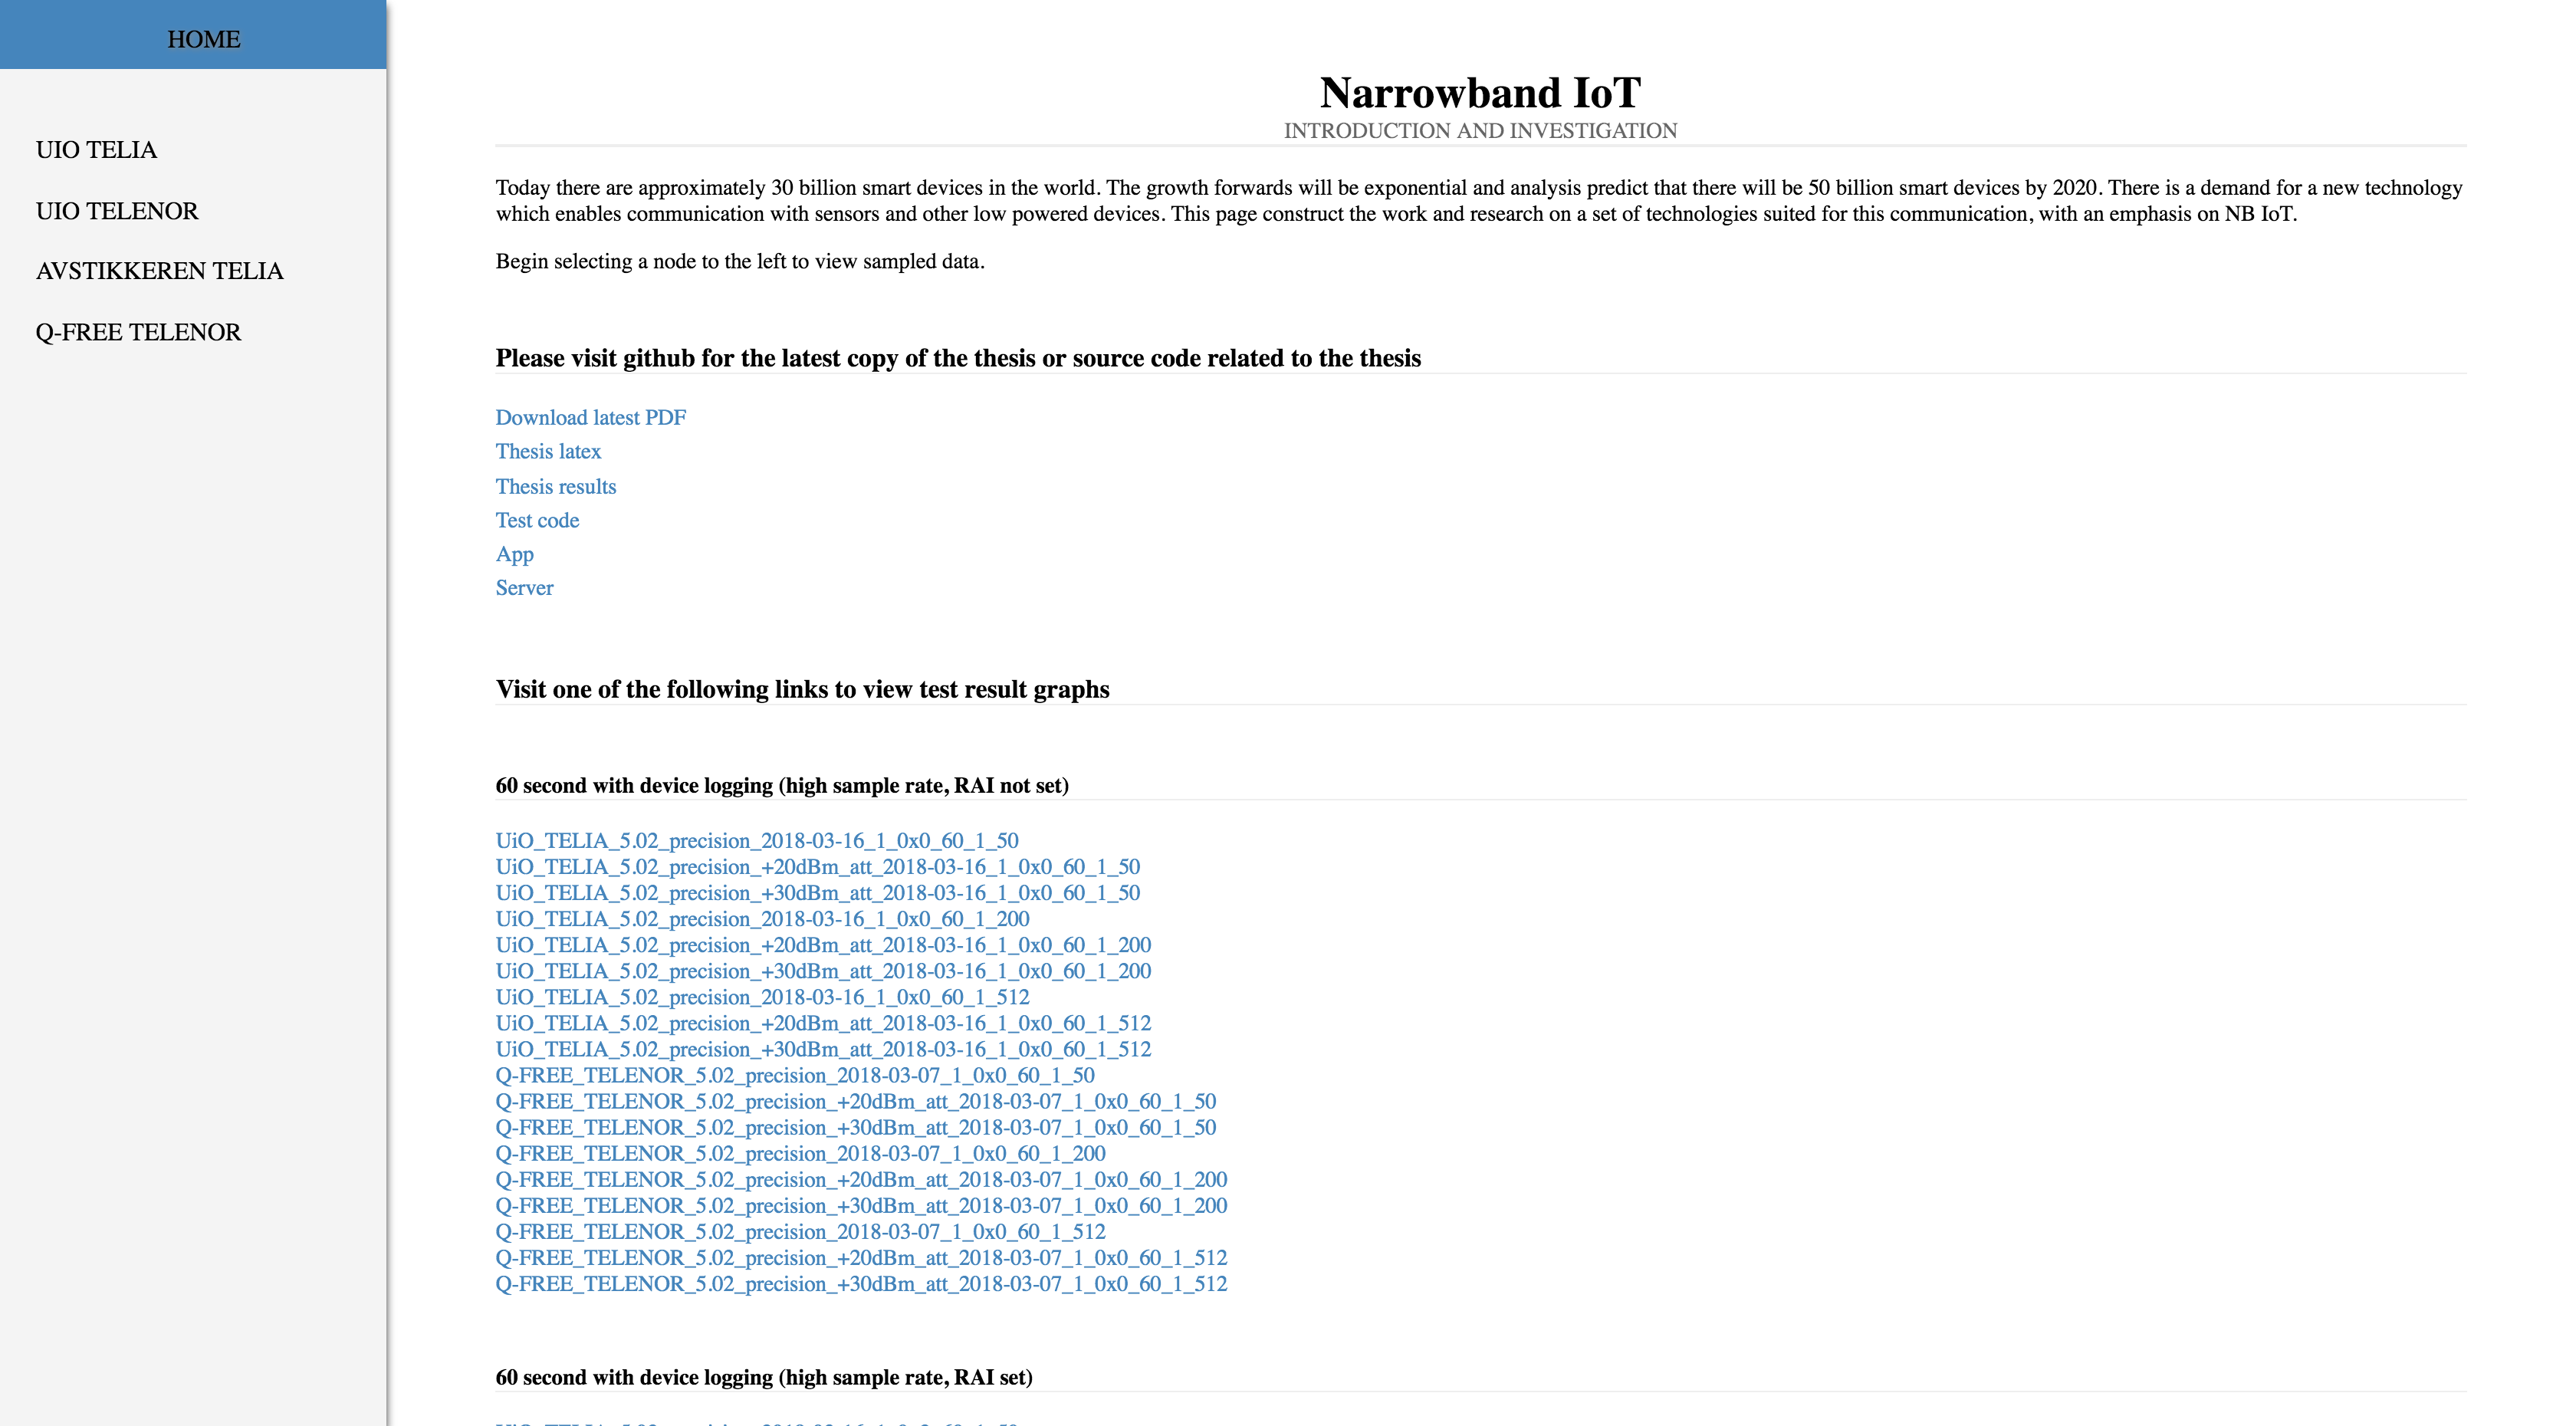
\includegraphics[width=12cm,height=8cm]{/Users/henninghakonsen/Dropbox/Masteroppgave/thesis/webapp/homepage.png}
  \caption{SensorApp homepage}
  \label{pic:homepage}
\end{figure}

\begin{figure}[H]
  \centering
  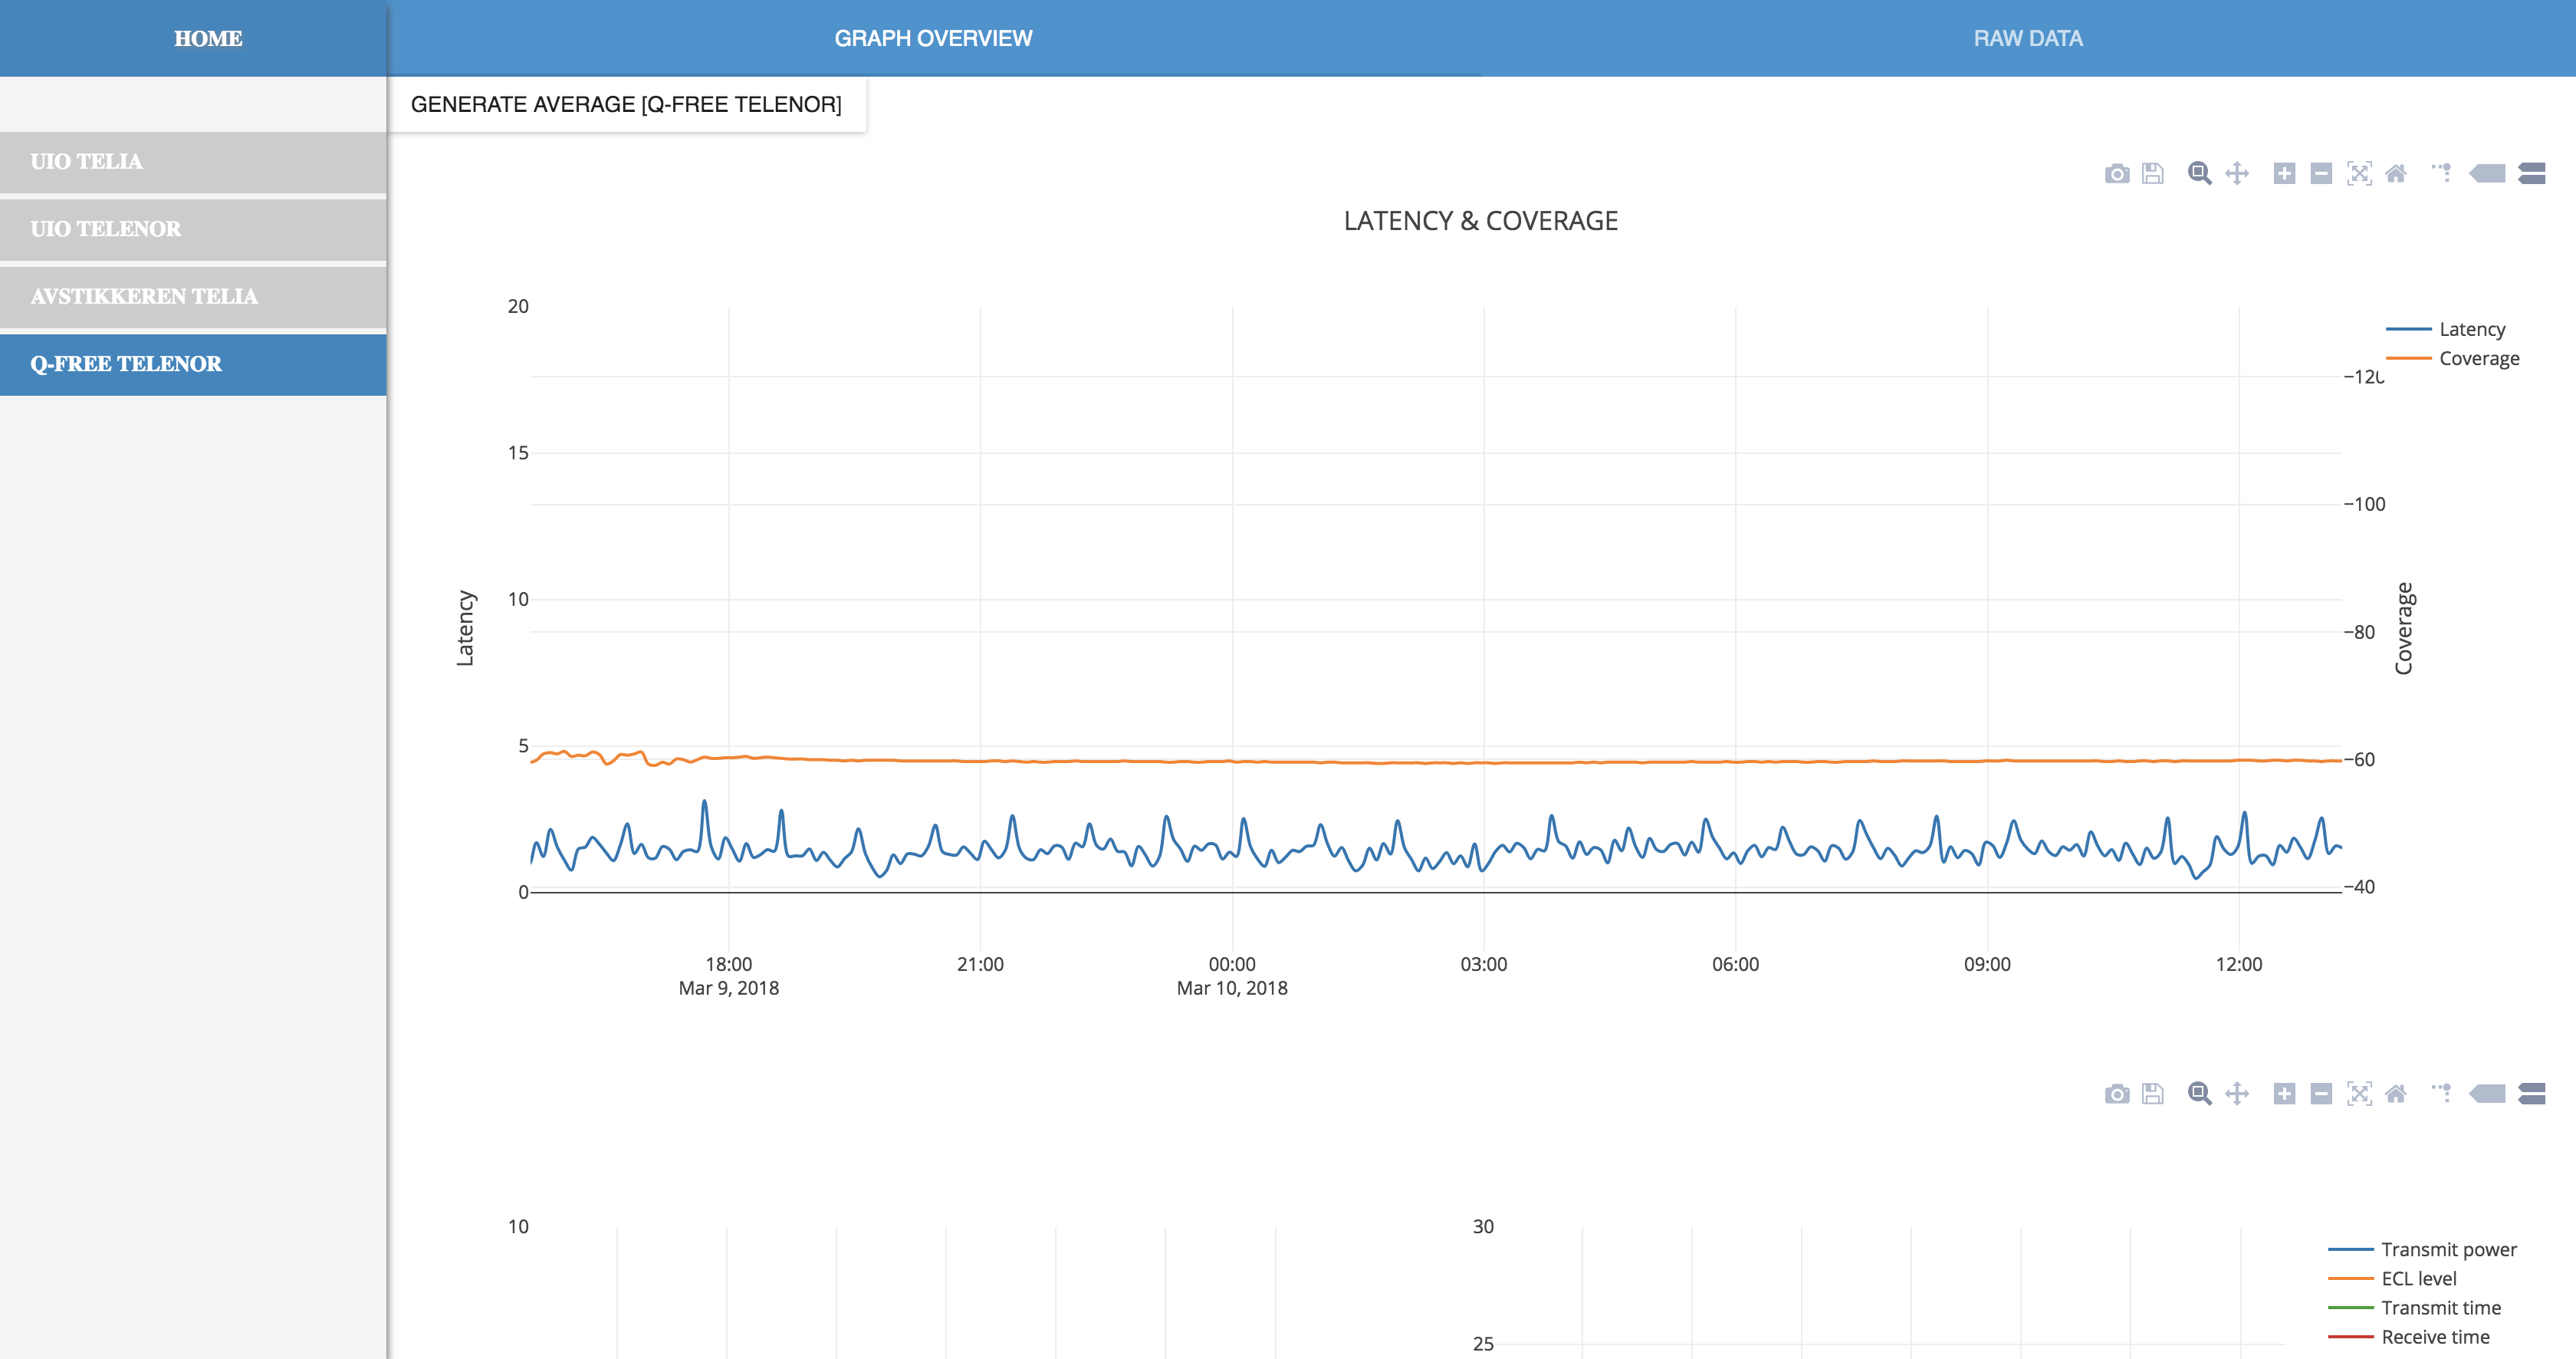
\includegraphics[width=12cm,height=8cm]{/Users/henninghakonsen/Dropbox/Masteroppgave/thesis/webapp/nodepage_1.png}
  \caption{SensorApp nodepage part 1}
  \label{pic:nodepage1}
\end{figure}

\begin{figure}[H]
  \centering
  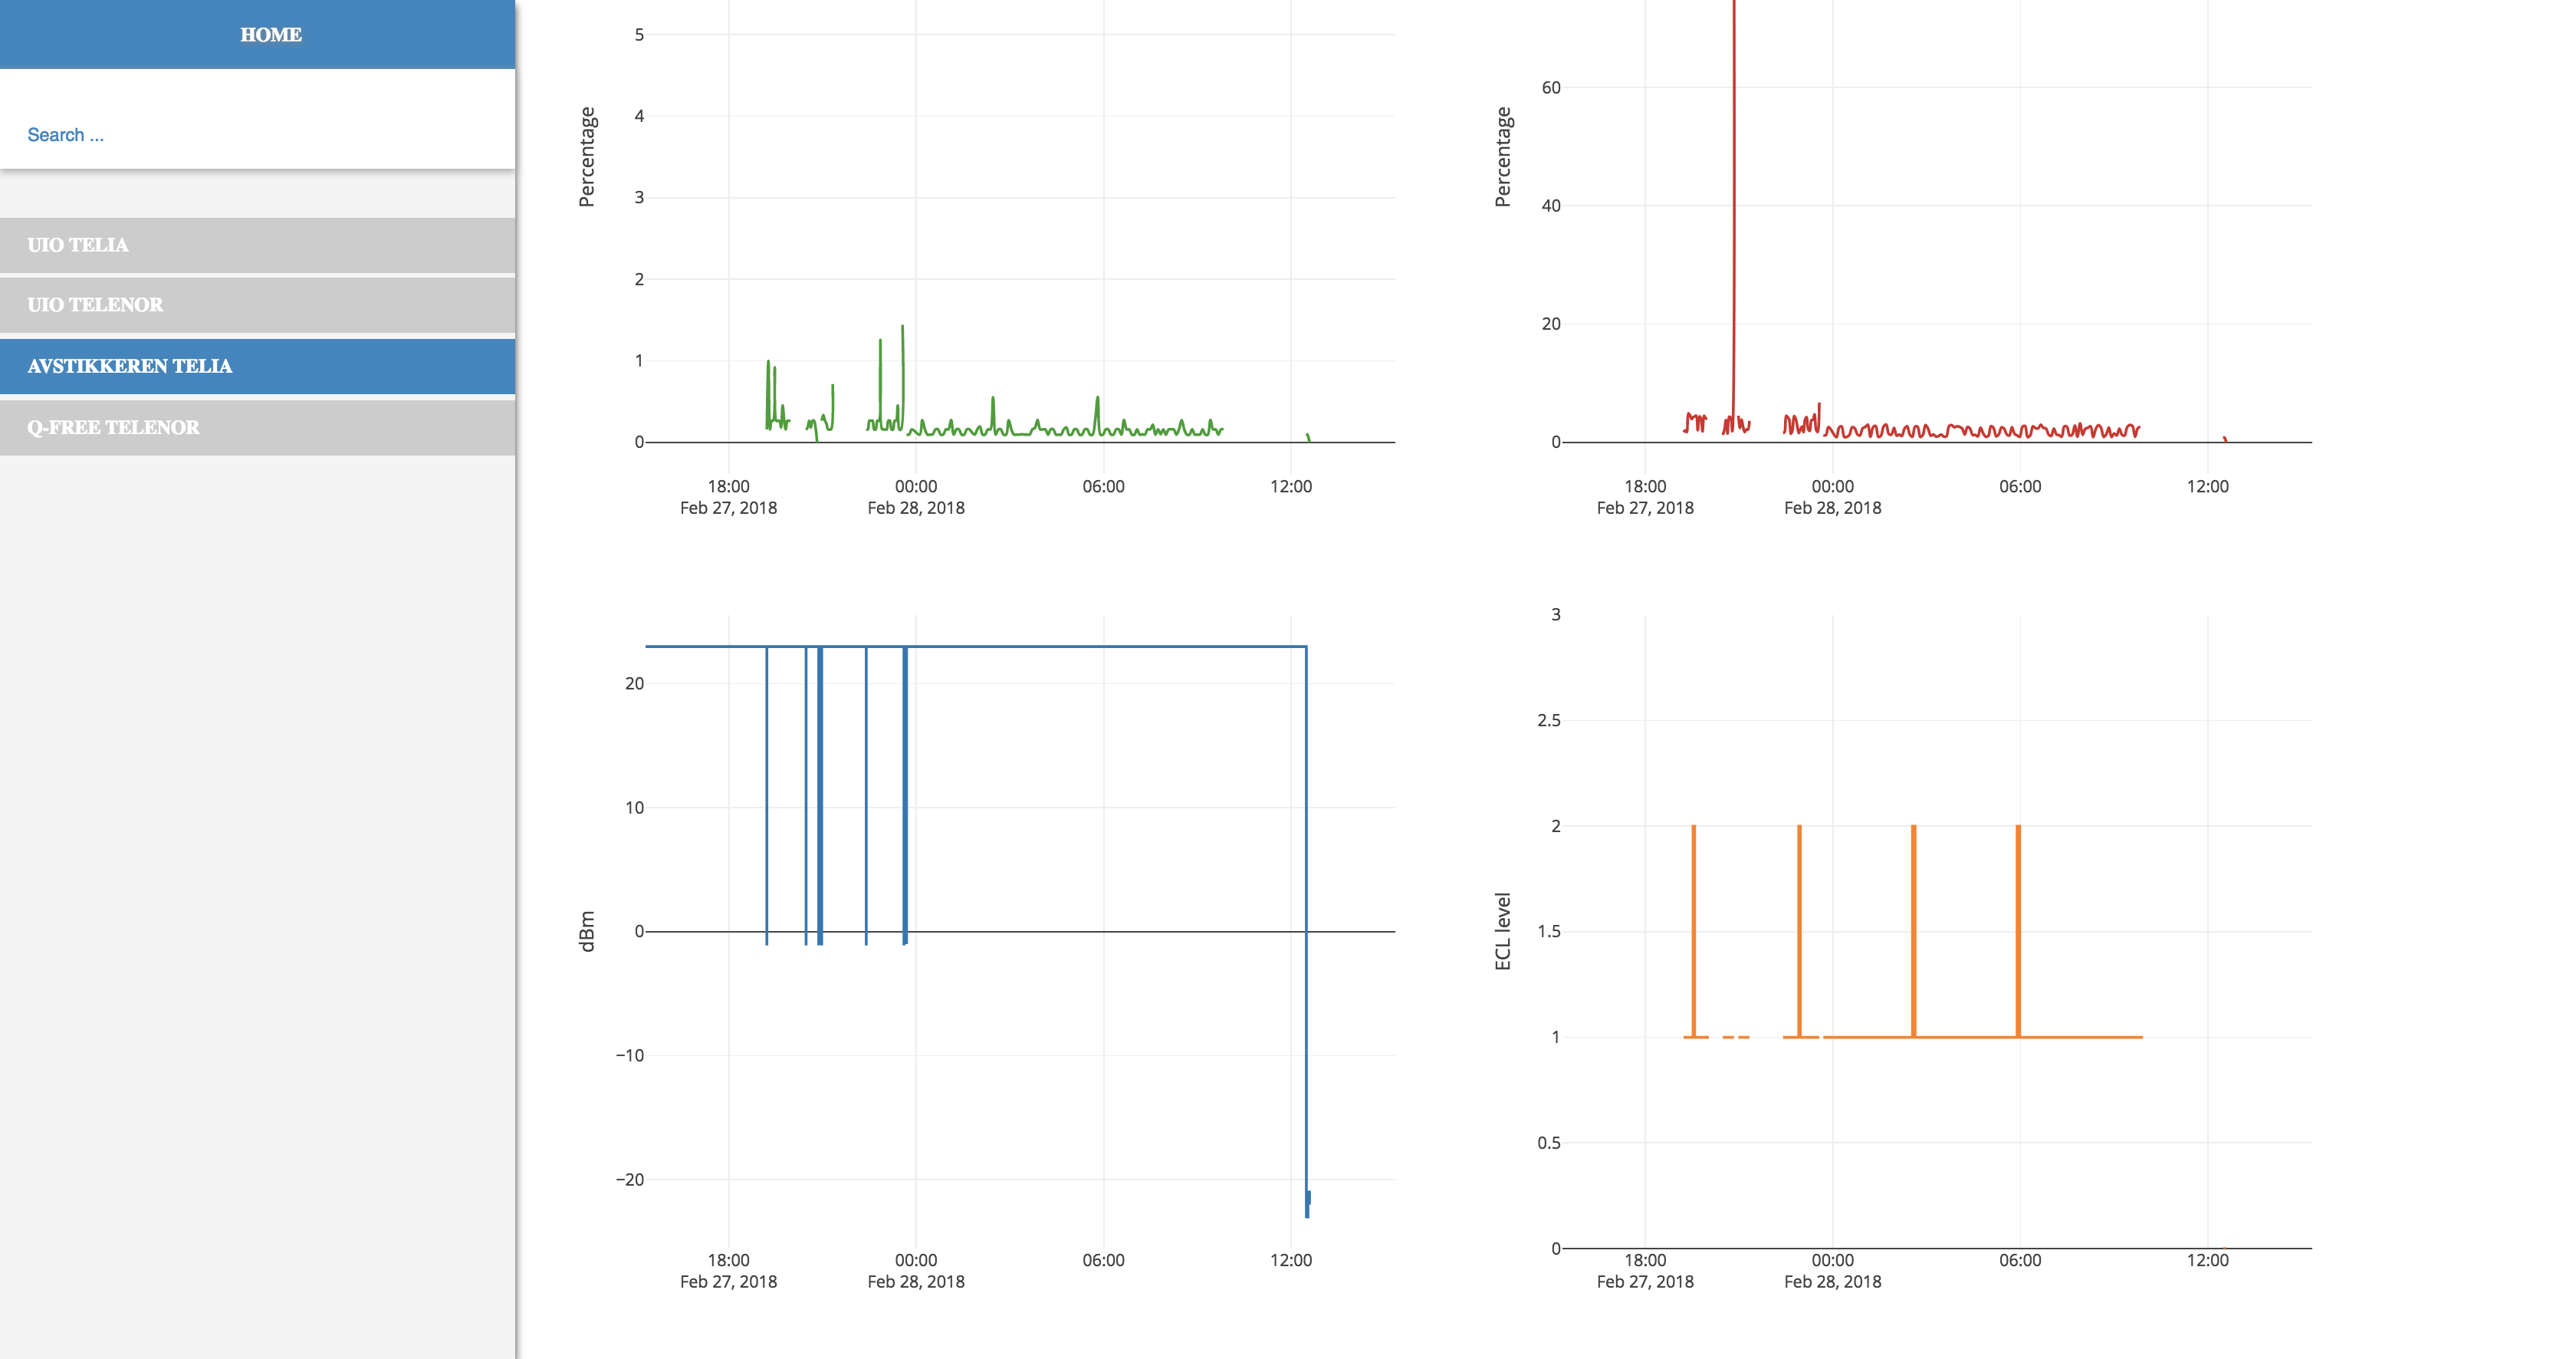
\includegraphics[width=12cm,height=8cm]{/Users/henninghakonsen/Dropbox/Masteroppgave/thesis/webapp/nodepage_2.png}
  \caption{SensorApp nodepage part 2}
  \label{pic:nodepage2}
\end{figure}

\subsubsection{Analysis} \label{ssection:analysis}
When selecting a node to explore you can explore the different graphs and we think this is a good way to display statistical data. The graphs data represents the output of the analysis on the server and we will try to describe what the graphs present and why we chose the different aspects of the behavior of the network. Remember that the data is mostly produced by \textbf{AT+NUESTATS}, so read, \vref{section:deviations}, for any deviations.

\paragraph{Coverage and Latency}
One of the main features of \acrshort{nb-iot} is coverage, hence we wanted to display coverage statistics over time. One interesting point of coverage is that it is closely related to the power usage of the device. The latency of \acrshort{nb-iot} is not a key feature, but the desired latency is under ten seconds according to the specifications\vref{datasheet:ubloxchip} and by displaying the latency in the same graph as coverage we can clearly see how the different coverage levels inflict latency in the network. The output of coverage and latency is directly from the output of \textbf{AT+NUESTATS}.

\paragraph{Recieve and transmit time}
The output from \textbf{AT+NUESTATS} gives us a counter from receive and transmit time in milliseconds. We used the value between each entry to calculate how much time the receive and transmit time. The analysis produces a percentage which relates to how much time the device was in receive or transmit state in one interval. This is also closely related to the coverage of the device and also the \acrshort{ecl} level which indicates the number of retransmits per packet sent. The reason why we would like to monitor this data is because the device will mostly use power in these periods, so if the device is active for longer periods in either receive or transmit state we know that the expected lifetime is degraded. Most of the time the active percentage will be low due to usage of release indicator flag and \acrshort{psm} mode, however if the transmit frequency is low the device will more frequently be in some kind of active state, hence the transmit and receive time will increase.

\paragraph{\acrshort{ecl}}
The coverage mode is also closely related to the power usage of the device and an important factor we could monitor. You can clearly see that the power usage increases when the device enters \acrshort{ecl} mode 1 and 2 in the testing section, \vref{section:testing}. The output of \acrshort{ecl} level directly from the output of \textbf{AT+NUESTATS}.

\paragraph{Transmit power}
The amount of power used for transmit is decided by software and is key to power usage. The output we get from \textbf{AT+NUESTATS} show us the latest transmit power level of the device. Sometimes the device will send a \acrfull{nack}, which is always sent with +23\acrshort{dbm} signal strength and is what \textbf{AT+NUESTATS} sometimes picks up as the latest transmit power level. In the long term tests with graphs from the web app the logging of transmit power might not be correct related to what transmit power level the device actually used for transmitting the packet. However in the section on detailed tests, \vref{section:detailedtest}, we will log the status of the device up to ten times a second which will give a better understanding of what is happening with the transmit power level.

%%HH add to this when the app is finished

\section{The chip}
In section \vref{paragraph:sensoroutline}, we looked at Q-Free's parking sensor, which houses a \acrshort{nb-iot} Ublox chip. The chip is produced by one of the leading producers in chip design and implementation. The chip features specifications in the same lines which \acrshort{nb-iot} specifies and we will use this chip for our testing. In this section we will look at the most essential modem commands for the \acrshort{nb-iot} chip. Modem commands are often referred to as AT-commands and we will use this notation throughout this paper. As mentioned in section, \vref{section:energysaving}, there are configurable timers in the network, as well as flags to keep in mind while developing software for low powered sensors. These parameters can be configured with AT-commands and has proven to give good results when taking power usage into consideration. In addition we will show you the AT-command for sending data, and how we intend to structure the data being sent.

In the following subsections we will give a brief introduction to the most important AT-commands taken from the AT Commands Manual for the \acrshort{nb-iot} chip \cite{atcommand:ubloxchip}. In section, \vref{section:testing}, we will give a more detailed description on the parameters used.

\subsection{Monitoring - NUESTATS}
Monitoring is an important part of developing and a way to verify that your software is running as optimal as possible. In our case we wanted a way to monitor the performance of the \acrshort{nb-iot} chip, hence we wanted to take advantage of the precise statistics given from the command \textbf{AT+NUESTATS}. According to the specifications of \acrshort{nb-iot}, there are a number of interesting thresholds and \textbf{AT+NUESTATS} will give us this information. In table, \vref{table:nuestats}, you can see the output of the command.

\begin{center} \label{table:nuestats}
  \begin{tabular}{ | l | m{10cm} | }
    \hline
    Power & NB-IoT signal power expressed in tenth of dBm \\
    \hline
    Total power & Total power within receive bandwidth expressed in tenth of dBm \\
    \hline
    Tx power & Transmit power expressed in tenth of dBm \\
    \hline
    Tx time & Elapsed transmit time since last power on event expressed in milliseconds \\
    \hline
    Rx time & Elapsed receive time since last power on event expressed in milliseconds \\
    \hline
    Cell id & Physical ID of the cell providing service to the module \\
    \hline
    \acrshort{ecl} & Last \acrshort{ecl} value \\
    \hline
    \acrshort{snr} & Last \acrfull{snr} value \\
    \hline
    \acrshort{earfcn} & Last \acrfull{earfcn} value \\
    \hline
    \acrshort{pci} & Last \acrfull{pci} value \\
    \hline
    \acrshort{rsrq} & Last \acrfull{rsrq} value \\
    \hline
  \end{tabular}
\end{center}

We believe that using \textbf{AT+NUESTATS} will give us accurate results. In addition we will use a high precision multimeter to monitor the current through the \acrshort{nb-iot} chip. We will introduce you to this device in section \vref{ssection:devices}. See section, \vref{section:deviations}, for any deviations.

\subsection{Time - CCLK}
Time is another tool we often use for developing software. We want to know how long a process endures, and in our case we want to monitor the latency of a send operation from the sensor to the server. With the AT-command \textbf{AT+CCLK?} we can read the time from the chip. This time is kept in sync with the network and stored in the \acrshort{mt}. The read operation returns a string with the time in the following format "yy/MM/dd,hh:mm:ss+TZ", where the characters represent, year, month, day, hours, minutes, seconds and time zone.

\subsection{\acrshort{ue} behaviour - NCONFIG}
With the AT-command \textbf{AT+NCONFIG} we are able to decide how we want the \acrshort{ue} to behave. HH skal vi bruke denne?

\subsection{CSQ} signal quality? Different from nuestats?

\subsection{\acrshort{edrx} settings - CEDRXS}
In section, \vref{ssection:edrx}, we explained how \acrshort{edrx} works and how we can configure the \acrshort{ue}. With the AT-command \textbf{AT+CEDRXS} we are able to define how \acrshort{edrx} is performed on the \acrshort{ue}. We can issue this AT-command, \textbf{AT+CEDRXS: 1, 5, "0101"}, to put the \acrshort{ue} into \acrshort{edrx} mode with cycle length of 163.84 seconds.

\subsection{\acrshort{psm} settings - CPSMS}
We can also define how \acrshort{psm} is used on the \acrshort{ue}. We can enable \acrshort{psm}, and set the timer \acrfull{T3412} with this command. If \acrshort{psm} is enabled, the device will enter deep sleep after expiry of the timer \acrfull{T3324}.

\subsection{NPOWERCLASS}
Force bands to use a given power class?

\subsection{Create socket - NSOCR}
Opens a port on the \acrshort{ue}, which enables data transfer on the given port. In our application we will open an \acrshort{udp} socket on a port. The port used can be a number between 0-65535, except for 5683 since this is used by the chip to send coap messages. The command returns a socket number which will be used for trailing send(NSOSTF) commands.

\subsection{Send command with flags - NSOSTF}
This AT-command enabled the device to send \acrshort{udp} packets on a given port with a flag. The command takes a set of parameters and the data in hexadecimal format. The parameters are, socket number(given by the AT-command NSOCR), remote IP address, remote port, flag, data length and actual data. The flag can be used to specify the behavior of the \acrshort{ue} after the data has been transmitted, see table, \vref{table:flag}, for details.

\begin{center} \label{table:flag}
  \begin{tabular}{ | l | m{10cm} | }
    \hline
    Mode & Description \\
    \hline
    0 & no flags are set \\
    \hline
    1 & Send message with high priority \\
    \hline
    2 & Indicate release after next message. This mode will put the \acrshort{ue} into \acrshort{psm} mode directly after transmitting data. Meaning less time in power heavy modes. \\
    \hline
    3 & Indicate release after next message has been replied to. \\
    \hline
  \end{tabular}
\end{center}

\subsection{Signaling connection status - CSCON}
We can verify the connection status of the \acrshort{ue} with the command AT+CSCON. If the reply of AT+CSCON? is 1 this means that the \acrshort{ue} is in RRC connected mode and is able to send and receive packets. If the reply is 0 this means that the \acrshort{ue} is in idle mode, hence the device uses little power and is inactive.

\subsection{Network registration status - CEREG}
We can verify the network registration status of the \acrshort{ue} with the command AT+CEREG. This command is very useul for detailed tests to check if the \acrshort{ue} is still connected to the network under the test.

\subsection{\acrshort{psm} status - NPSMR}
Gives us the status of \acrshort{psm} on the device. It will return 1,1 if the device is in \acrshort{psm} mode which means that the power usage should be very low.

\chapter{Testing} \label{section:testing}
%%HH change introduction to fit the tests we are performing
In the test chapter we will be looking at tests, with as many scenarios as possible. We will describe testing environment, devices and parameters that effects the tests. At the end we will try to conclude wether or not \acrshort{nb-iot} is as promising as it looks on paper.

The test phase began early January and was completed early March. The reason for the long test phase was due to a number of things. First of all the hardware and software related to \acrshort{nb-iot} was not available on a stable platform until late 2017, and Telenor and Telia had limited \acrshort{nb-iot} enabled base stations. Even at the beginning of 2018 the devices acquired were not production ready, hence our tests were somewhat inadmissible. However the equipment was at a stage where the error rate was very low and the test phase could start. Given the hypothesis we needed to test the chip and the network with good equipment and at several locations. In section, \vref{section:testingenv}, we will give you an overview of the testing premissis and the devices used.

\section{Testing environment} \label{section:testingenv}
The testing took place at several locations - UiO, at my apartment at Lambertseter and at Q-Free's office by Solli Plass. With three locations and two network providers we could collect more information, hence we got a better understanding of the results.

Not all base stations in these areas are \acrshort{nb-iot} enabled, but you will see that different coverage levels will affect the results and we can compare the results to a "perfect world"/specification setup. The coverage of the chip is related to the supplied antenna and the direction of this. With the \acrshort{nb-iot} development kit there was an antenna and we could position it the way with the best result. See pictures, \vref{pic:uio_nbiot_setup} and \vref{pic:antenna_position}, to see the setup at UiO.

\begin{figure}[ht]
  \centering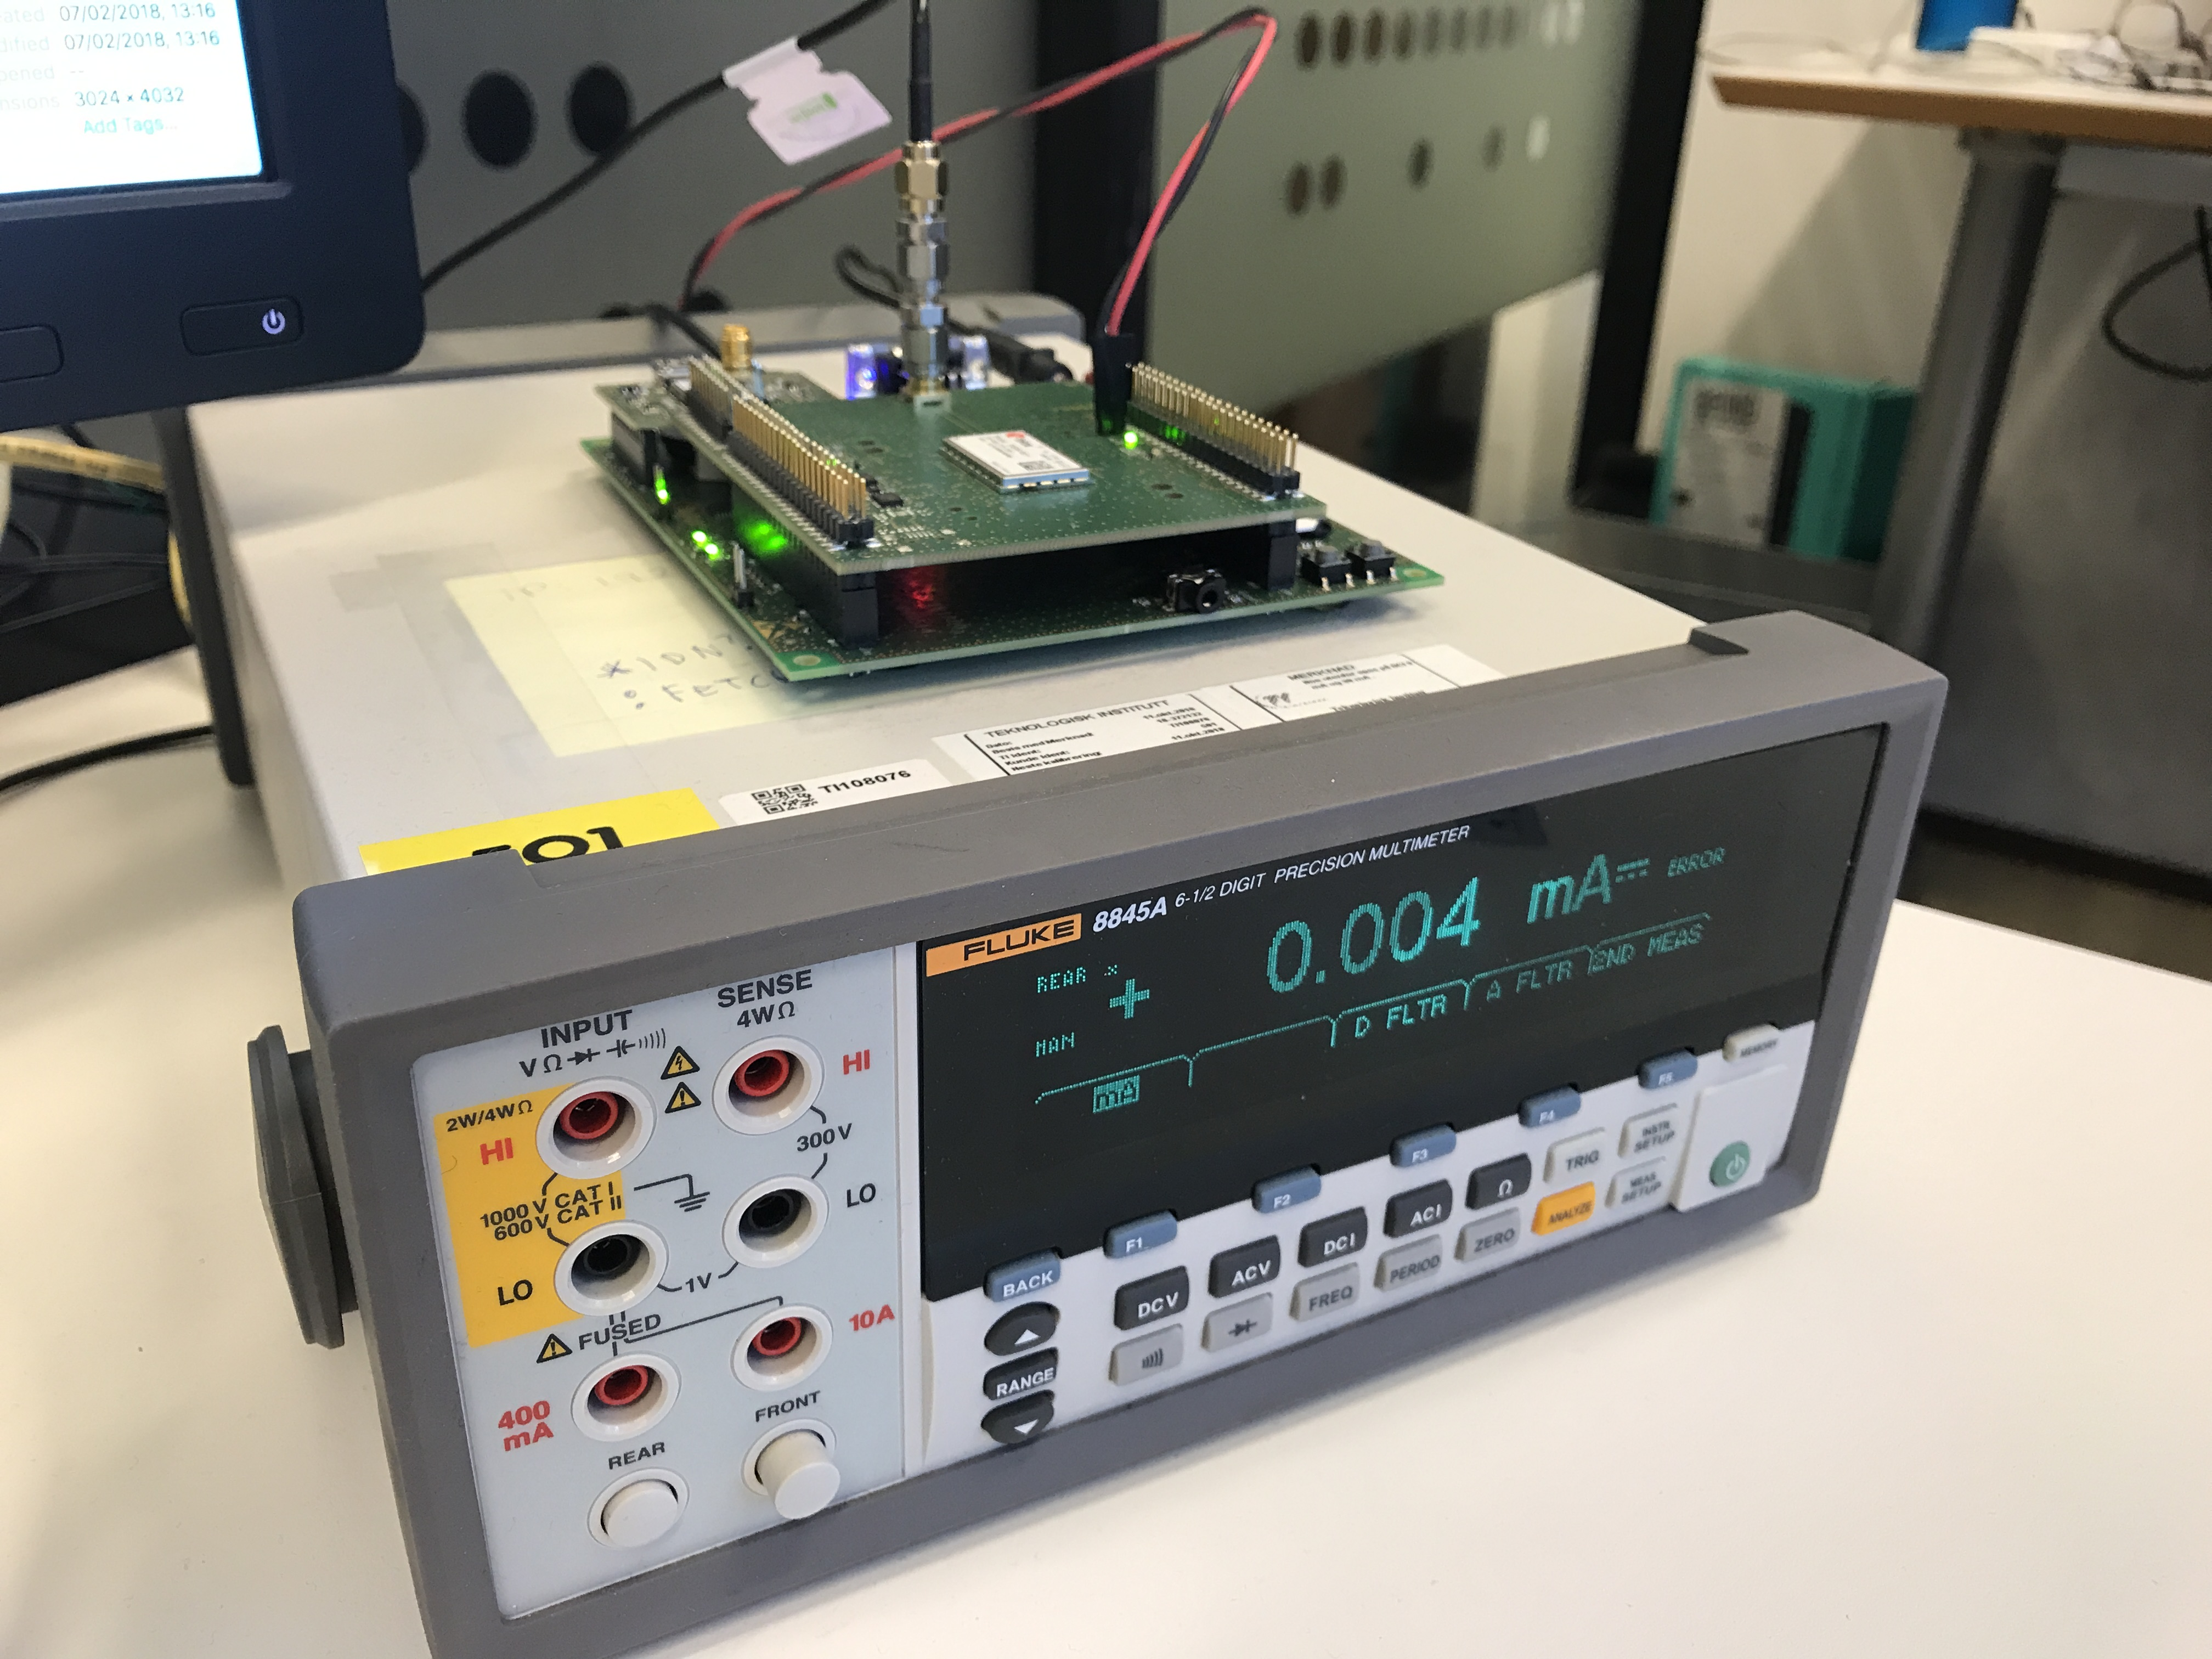
\includegraphics[width=12cm,height=8cm]{/Users/henninghakonsen/Dropbox/Masteroppgave/thesis/latex/images/uio_nbiot_setup.jpg}
  \caption{\acrshort{nb-iot} and multimeter setup}
  \label{pic:uio_nbiot_setup}
\end{figure}

\begin{figure}[ht]
  \centering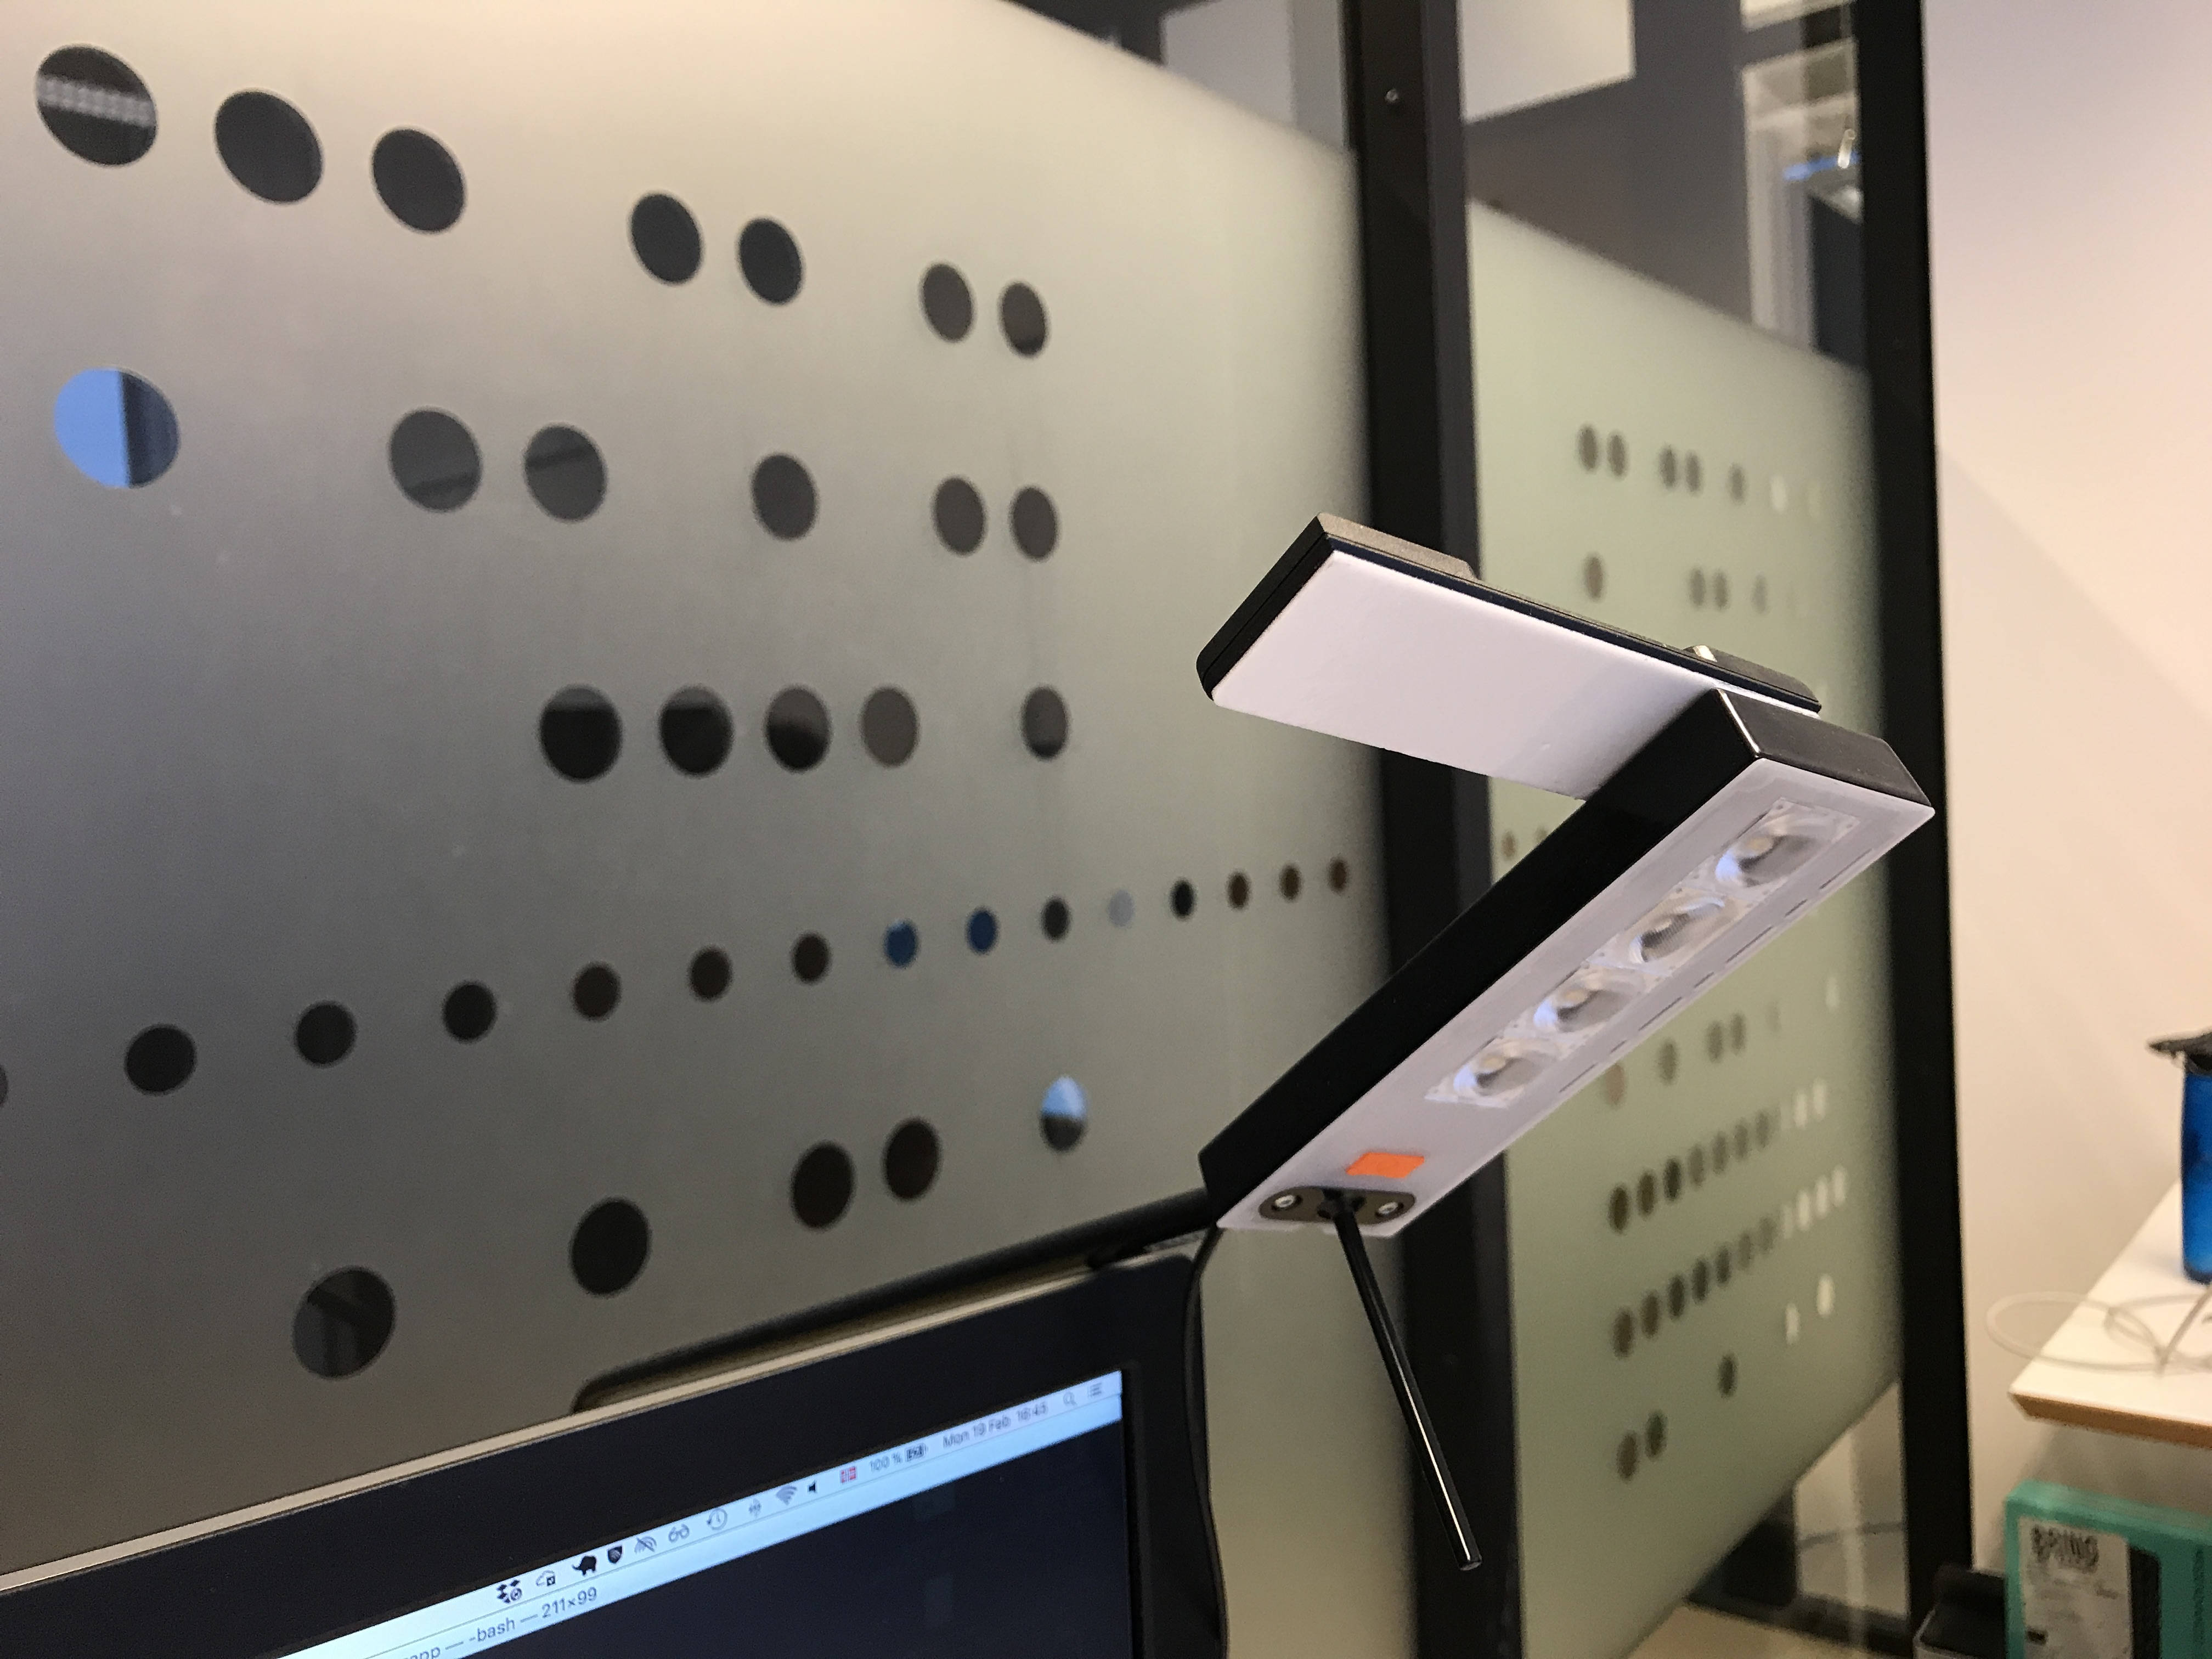
\includegraphics[width=12cm,height=8cm]{/Users/henninghakonsen/Dropbox/Masteroppgave/thesis/latex/images/antenna_position.jpg}
  \caption{\acrshort{nb-iot} antenna position}
  \label{pic:antenna_position}
\end{figure}

HH add maps with base stations

\subsection{Devices} \label{ssection:devices}
\subsubsection{\acrshort{nb-iot} development kit}
We are using a development kit from Ublox with their \acrshort{nb-iot} chip called SARA N2, see picture \vref{pic:nbiotdevkit}. The development kit is connected to a computer over USB and allows us to send and receive data through the serial port of the chip. We will use this setup for both detailed tests such as packet size tracking, coverage tracking and network provider tracking, and use it for longer tests where we continuously send messages with a more practical frequency to the server. The computer will run different python programs to test the different challenges and most of the time we will send \textbf{AT+NUESTATS} to the application server so that we can process the information. In certain cases we will also log test runs on the computer for detailed graphs of the behavior of the chip.

\begin{figure}[ht]
  \centering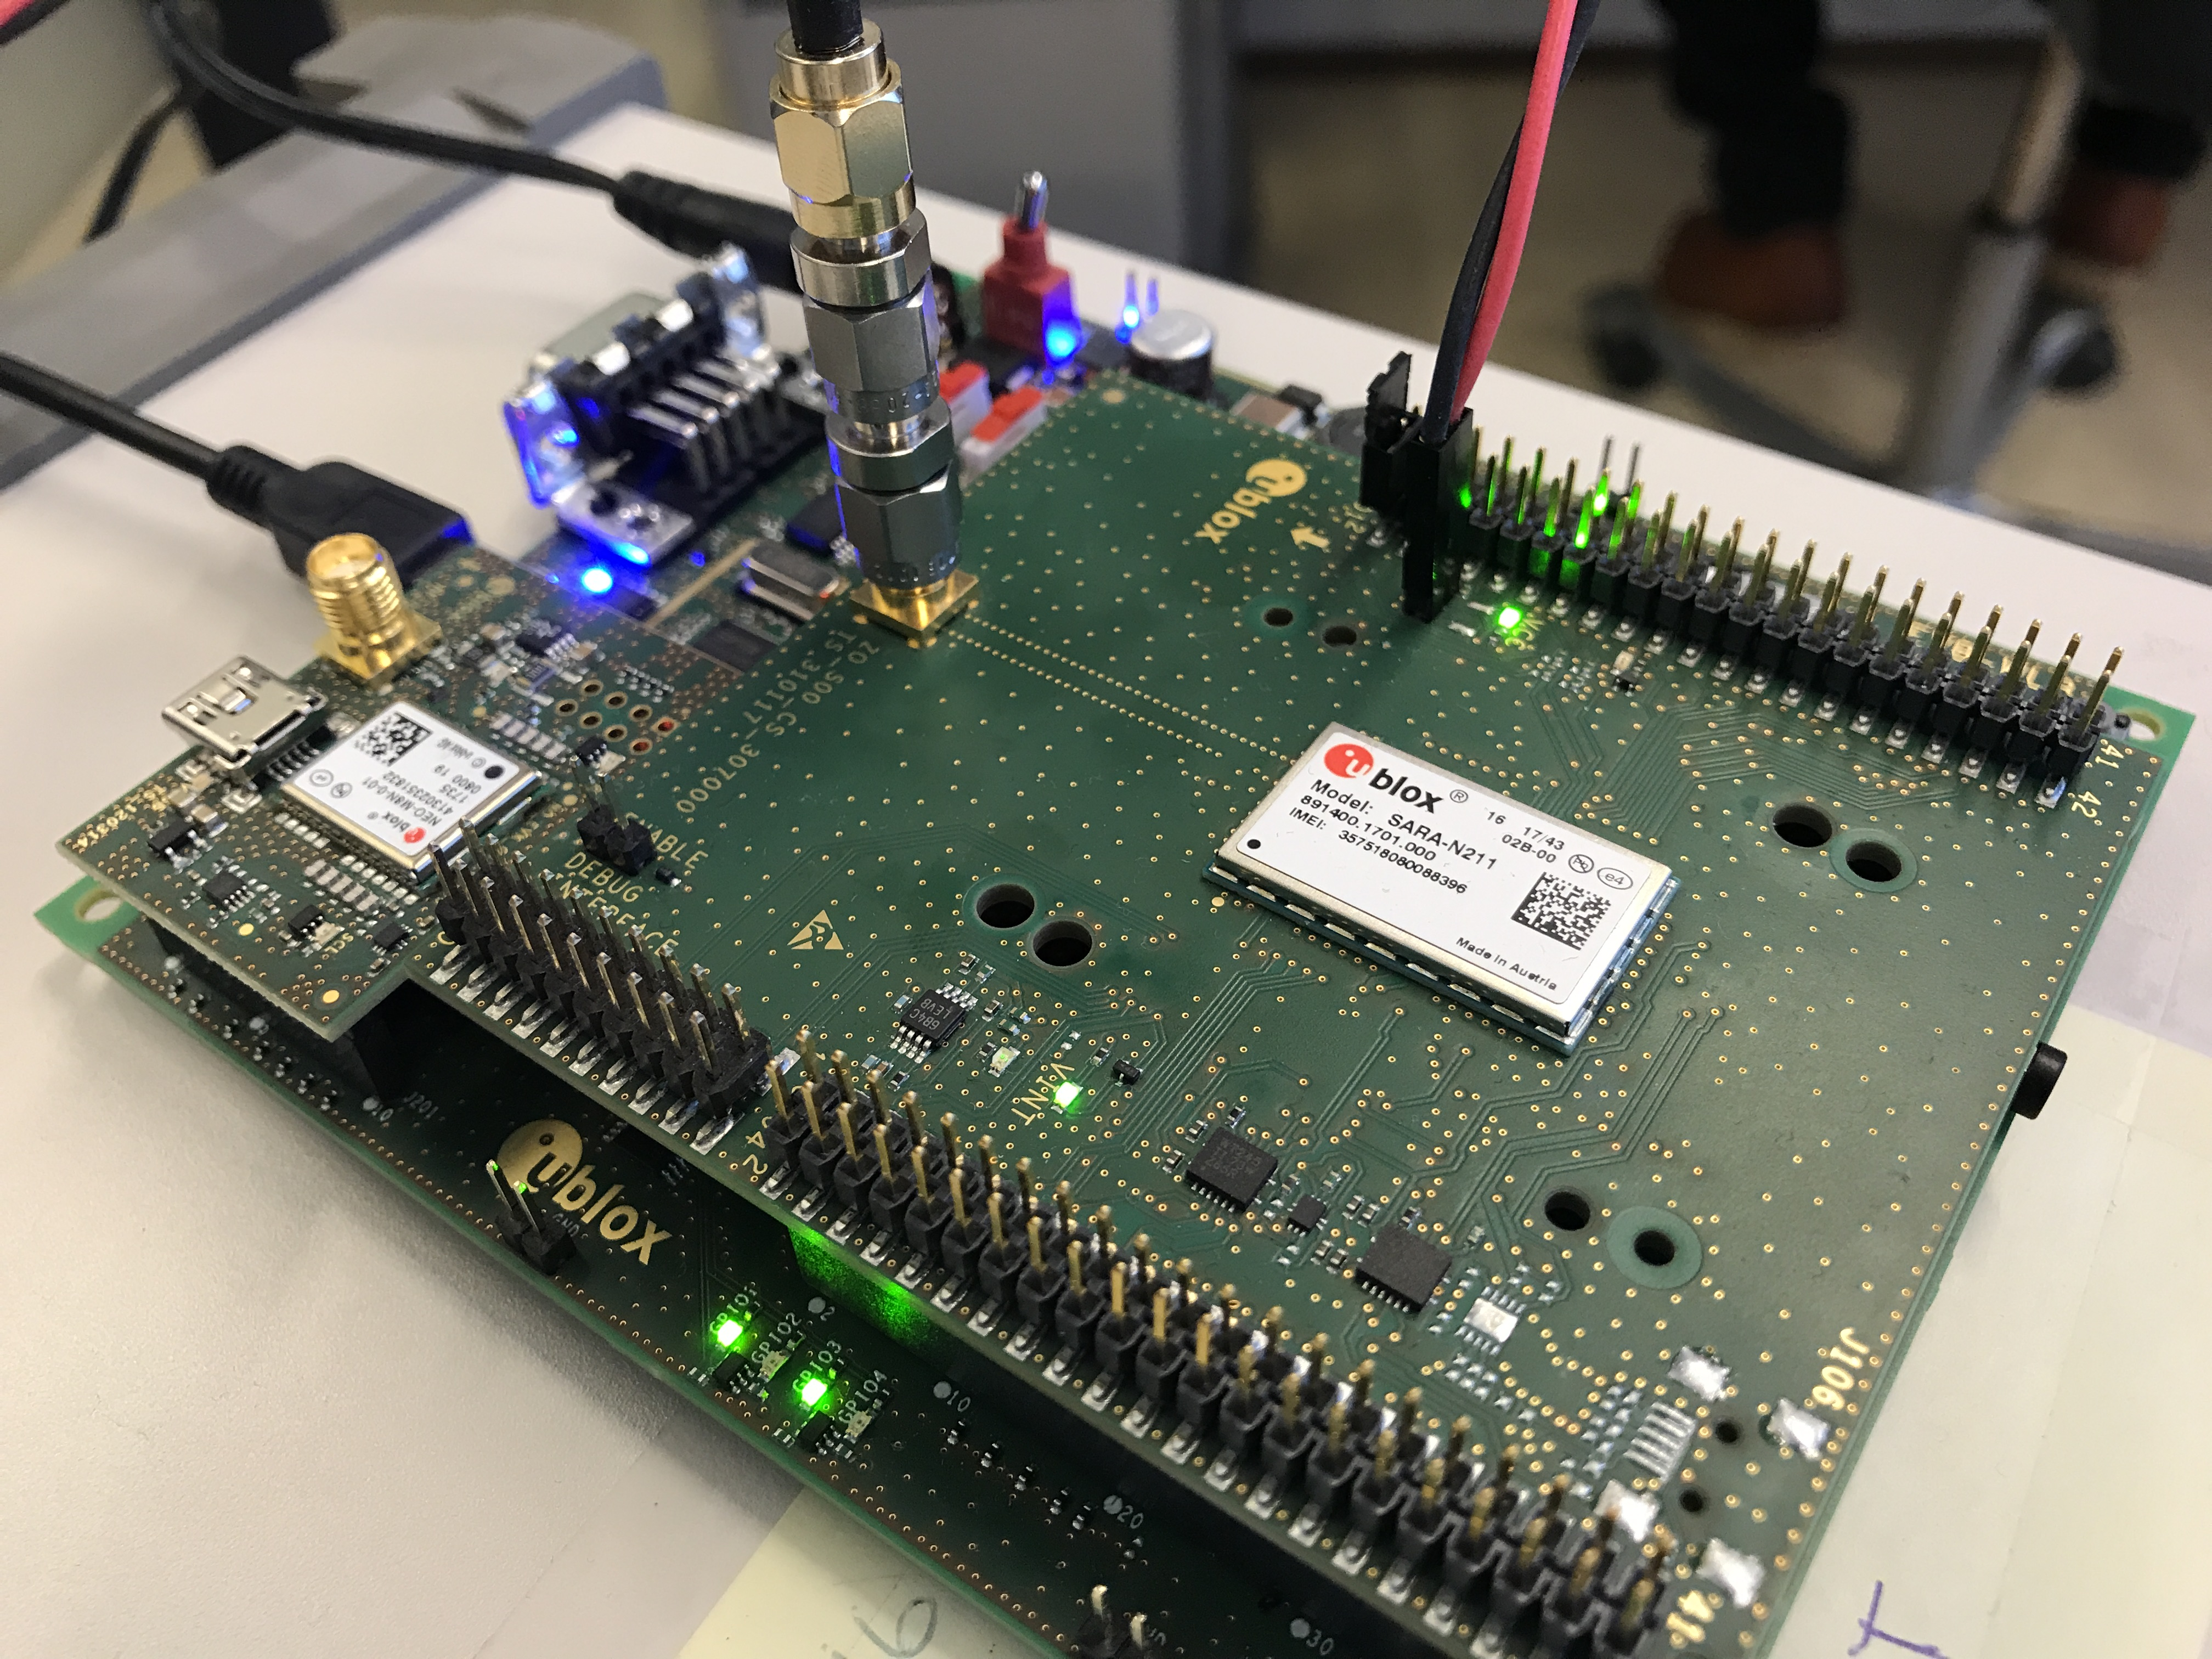
\includegraphics[width=12cm,height=8cm]{/Users/henninghakonsen/Dropbox/Masteroppgave/thesis/latex/images/nbiot_devkit.jpg}
  \caption{Ublox \acrshort{nb-iot} development kit}
  \label{pic:nbiotdevkit}
\end{figure}

\subsubsection{Fluke precision multimeter}
Q-Free was so lucky to borrow a precision multimeter from ... (HH - OML) which we used to measure the current through the \acrshort{nb-iot} chip. With the multimeter we managed to pinpoint different stages of the chip. In addition we added corresponding statistics from \textbf{AT+NUESTATS} which increased the precision. As sketched in figure, \vref{figure:labsetup}, we connected the multimeter to the computer using an ethernet cable, enabling us to fetch readings from the device. Depending on the selected precision of the measurements we collected between 30-300 samples per second. The most detailed tests required high sample rate, while we used higher precision measurements on longer tests. The device responded on commands much like a \acrfull{repl}, where you issue a request with a command and the device will respond with an answer. In table, \vref{table:fluke_commands}, you can see the commands we used and a short description related to them.

\begin{center} \label{table:fluke_commands}
  \begin{tabular}{ | l | m{10cm} | }
    \hline
    Command & Description \\
    \hline
    :INIT & Clears old readings \\
    \hline
    :FETCH? & Fetches all readings from the device. The response is a long string with numbers divided with "," \\
    \hline
  \end{tabular}
\end{center}

\subsection{Writing tests}
You should at this point have an idea of the setup and how things are connected, if not, see figure \vref{figure:labsetup} for description.

\begin{figure}[ht]
  \centering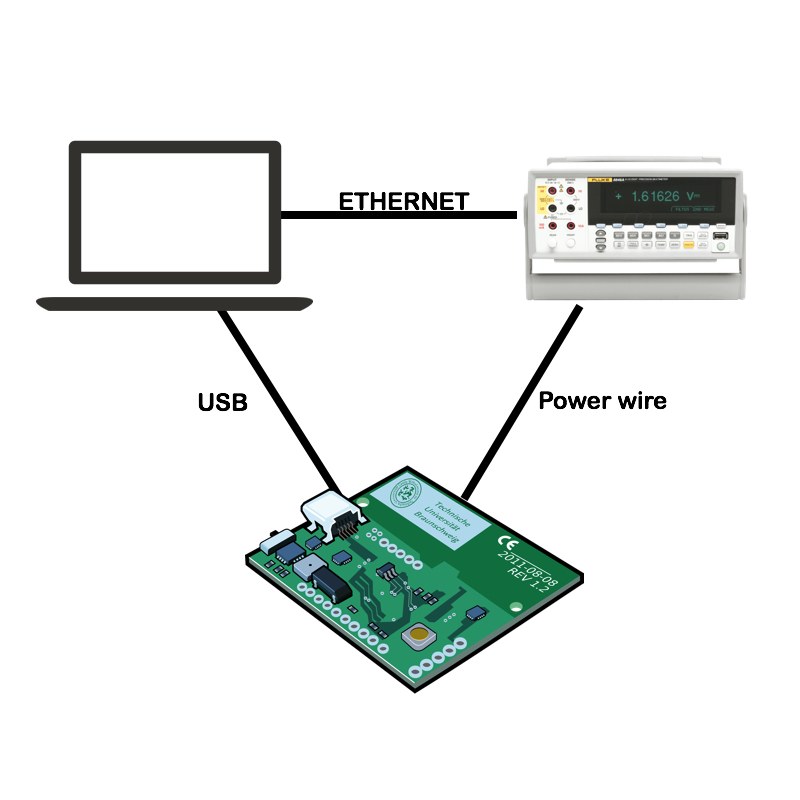
\includegraphics[width=10cm,height=10cm]{/Users/henninghakonsen/Dropbox/Masteroppgave/thesis/latex/images/labsetup.jpg}
  \caption{Lab setup \cite{pcpng35052:online} \cite{fluke88435:online} \cite{ingagrue31:online}}
  \label{figure:labsetup}
\end{figure}

We started writing test features for the development kit using python. We setup a connection between the program and the serial port and configure the device to make sure that everything is according to our setup, see code \vref{code:modem}.

\begin{lstlisting}[caption={Development kit initiation},label={code:modem},language=Python]
uart_modem = serial.Serial('/dev/tty.usbserial-146100', 9600, timeout = 0)
uart_modem.close()
uart_modem.open()
uart_modem.flushInput()
uart_modem.flushOutput()
\end{lstlisting}

We started experimenting with different AT commands and created small programs to test the functionality of the chip and the connection towards the server. We created a simple program which sent \textbf{AT+NUESTATS} to the application server and went on transforming this program to helper methods we could use later on. A sample packet with a COAP header would look something like the example, \vref{samplecommand}, where the payload is converted to hexadecimal. We used some time creating the correct COAP packet for the server to accept it as a COAP packet. If you don't want to use COAP you can simply fill the payload with data without the COAP header, but this means that you are missing the features of COAP which could be beneficial for your application. Dropping the COAP header means that you are sending a pure \acrshort{udp} packet through the network and it is harder to verify the packet when it is received on an eventual application server.

\begin{lstlisting}[caption={Sample transmit 158.39.77.97:5683, 88 bytes},label={samplecommand},language=Python]
  AT+NSOSTF=0,"158.39.77.97",5683,0x0,88,"500230
  30B131112AFF2D313039365F2D313034325F3233305F39
  3732315F37363838305F33343433393435325F315F3132
  335F363235325F39385F2D3130385F31382F30322F3139
  2C31363A31363A35362B30305F31325F"
\end{lstlisting}

We proceeded working on communication towards the multimeter, which was quite easy. The multimeter was given an \acrshort{ip} address which was related to the \acrshort{ip} address of the connected machine. Creating a socket to this IP address in python and connecting to it was simple. The test programs would start off by clear all buffers with \textbf{:INIT} and then fetch for data on a regular interval with \textbf{:FETCH?; :INIT}. With each reading we converted the string into a list of numbers which we appended to a global list of readings. We found that fetching for new data every 5th second was a good tradeoff between fetching all the time and very rare. We added these functions to the helper file, \textbf{nbiot\_labtest\_helpers.py}, and went on writing a couple of programs to monitor the behaviour of the chip.

%%HH
\paragraph{\textbf{nbiot\_labtest.py}}
This program continuously transmits packets over \acrshort{nb-iot} - either status packets towards the server or random data of different sizes. It enabled us to test different scenarios and log the results in a representable way with graphs. The program uses The program takes in a list of parameters described in table, \vref{table:labtestparameters}.

\begin{center} \label{table:labtestparameters}
  \begin{tabular}{ | l | m{10cm} | }
    \hline
    Parameter & Description \\
    \hline
    -id & ID which you want to POST towards the server. Default: 0 \\
    \hline
    -gn & Output graph name. The supplied name will lead the heading, followed by a list of the rest of the parameters. \\
    \hline
    -d & Set the desired delay between each iteration. Default: 5 \\
    \hline
    -i & Set the desired iterations. Default: -1 which means that the program will loop until the user presses ctrl+c \\
    \hline
    -b & Set the desired length of the payload in bytes. If 0 is requested, statistics from \textbf{NUESTATS} will be sent to server. Default: 100 \\
    \hline
    -r & Set release indicator. Default: false \\
    \hline
    -l & Set device logging. Default: false \\
    \hline
  \end{tabular}
\end{center}

\section{Detailed \acrshort{nb-iot} tests} \label{section:detailedtest}
In this section we will investigate how the \acrshort{nb-iot} chip handles normal usage and edge cases where non default behavior is activated.

\subsection{Latency test} \label{ssection:latencytest}

\subsection{Coverage test} \label{ssection:coveragetest}
\acrshort{ecl} modes

\subsection{Packet size} \label{ssection:packetsize}
Try different packet sizes and check power usage (are there any perfect packet sizes? - I think 64B is one datablock)

\subsection{Reboot of sensor?} \label{ssection:reboottest}

\subsection{Cell selection test} \label{ssection:cellselectiontest}

\subsection{Downtime test} \label{ssection:downtimetest}


\section{Long term tests} \label{section:longtermtest}

\subsection{Coverage and latency}

\subsection{Operating modes}

\subsection{Cell selection}

\subsection{Uptime}

\section{Deviations} \label{section:deviations}
\subsection{Imprecise clock}
With the command \textbf{AT+CLOCK?} we get the time from the network. This timestamp is not a precise time, but we believe that it is good enough to test the specified 10 second latency in the \acrshort{nb-iot} network. When doing the detailed tests we tried to verify that the timestamp received from the network was accurate. In most cases the time was very precise, only with a deviation of 10ms. HH verify

\subsection{Network load}
Since the \acrshort{nb-iot} network was not in production at the time of the tests, the network was not heavily loaded. This means that the latency could be a bit higher with more general activity on the network. When the network is available the latency should be low and that is our impression on the \acrshort{nb-iot} network as well. HH verify

\subsection{Network density}
Since the network was not in production, the density of the cell towers with \acrshort{nb-iot} were limited. In the future all cells will implement \acrshort{nb-iot}, meaning that the uptime will increase. The coverage will probably also increase since we could possibly connect to a closer cell tower if the density is higher.

load on server + server park

\section{Early test faults}
Changing cell when not in bad coverage
Looses connection to network and sudden bursts of packets are received
Some packet loss, which should not appear since the load on this network was low in the test period.


\part{Conclusion}                     %% ... or Konklusjon

\chapter{Results}                     %% ... or ??


\backmatter{}
\printbibliography
\printglossary[type=\acronymtype]
\end{document}
